%&preformat-disser
\RequirePackage[l2tabu,orthodox]{nag} % Раскомментировав, можно в логе получать рекомендации относительно правильного использования пакетов и предупреждения об устаревших и нерекомендуемых пакетах
% Формат А4, 14pt (ГОСТ Р 7.0.11-2011, 5.3.6)
\documentclass[a4paper,14pt,oneside,openany]{memoir}

%%%%%%%%%%%%%%%%%%%%%%%%%%%%%%%%%%%%%%%%%%%%%%%%%%%%%%%%%%%%%%%%%%%%%%%%%%%%%%%%
%%%% Файл упрощённых настроек шаблона, общих для диссертации и автореферата %%%%
%%%%%%%%%%%%%%%%%%%%%%%%%%%%%%%%%%%%%%%%%%%%%%%%%%%%%%%%%%%%%%%%%%%%%%%%%%%%%%%%

%%% Режим черновика %%%
\makeatletter
\@ifundefined{c@draft}{
  \newcounter{draft}
  \setcounter{draft}{0}  % 0 --- чистовик (максимальное соблюдение ГОСТ)
                         % 1 --- черновик (отклонения от ГОСТ, но быстрая
                         %       сборка итоговых PDF)
}{}
\makeatother

%%% Пометки в тексте %%%
\makeatletter
\@ifundefined{c@showmarkup}{
  \newcounter{showmarkup}
  \setcounter{showmarkup}{0}  % 0 --- скрыть пометки
                              % 1 --- показывать пометки
}{}
\makeatother

%%% Использование в pdflatex шрифтов не по-умолчанию %%%
\makeatletter
\@ifundefined{c@usealtfont}{
  \newcounter{usealtfont}
  \setcounter{usealtfont}{1}    % 0 --- шрифты на базе Computer Modern
                                % 1 --- использовать пакет pscyr, при его
                                %       наличии
                                % 2 --- использовать пакет XCharter, при наличии
                                %       подходящей версии
}{}
\makeatother

%%% Использование в xelatex и lualatex семейств шрифтов %%%
\makeatletter
\@ifundefined{c@fontfamily}{
  \newcounter{fontfamily}
  \setcounter{fontfamily}{1}  % 0 --- CMU семейство. Используется как fallback;
                              % 1 --- Шрифты от MS (Times New Roman и компания)
                              % 2 --- Семейство Liberation
}{}
\makeatother

%%% Библиография %%%
\makeatletter
\@ifundefined{c@bibliosel}{
  \newcounter{bibliosel}
  \setcounter{bibliosel}{1}   % 0 --- встроенная реализация с загрузкой файла
                              %       через движок bibtex8;
                              % 1 --- реализация пакетом biblatex через движок
                              %       biber
}{}
\makeatother

%%% Вывод типов ссылок в библиографии %%%
\makeatletter
\@ifundefined{c@mediadisplay}{
  \newcounter{mediadisplay}
  \setcounter{mediadisplay}{0}   % 0 --- не делать ничего; надписи [Текст] и
                                 %       [Эл. ресурс] будут выводиться только в ссылках с
                                 %       заполненным полем `media`;
                                 % 1 --- автоматически добавлять надпись [Текст] к ссылкам с
                                 %       незаполненным полем `media`; таким образом, у всех
                                 %       источников будет указан тип, что соответствует
                                 %       требованиям ГОСТ
                                 % 2 --- автоматически удалять надписи [Текст], [Эл. Ресурс] и др.;
                                 %       не соответствует ГОСТ
                                 % 3 --- автоматически удалять надпись [Текст];
                                 %       не соответствует ГОСТ
                                 % 4 --- автоматически удалять надпись [Эл. Ресурс];
                                 %       не соответствует ГОСТ
}{}
\makeatother

%%% Предкомпиляция tikz рисунков для ускорения работы %%%
\makeatletter
\@ifundefined{c@imgprecompile}{
  \newcounter{imgprecompile}
  \setcounter{imgprecompile}{0}   % 0 --- без предкомпиляции;
                                  % 1 --- пользоваться предварительно
                                  %       скомпилированными pdf вместо генерации
                                  %       заново из tikz
}{}
\makeatother
            % общие настройки шаблона
\input{common/packages}         % Пакеты общие для диссертации и автореферата
\synopsisfalse                      % Этот документ --- не автореферат
\input{Dissertation/dispackages}    % Пакеты для диссертации
\usepackage{fr-longtable}    %ради \endlasthead

% Листинги с исходным кодом программ
\usepackage{fancyvrb}
\usepackage{listings}
\lccode`\~=0\relax %Без этого хака из-за особенностей пакета listings перестают работать конструкции с \MakeLowercase и т. п. в (xe|lua)latex

% Русская традиция начертания греческих букв
\usepackage{upgreek} % прямые греческие ради русской традиции

%%% Микротипографика
%\ifnumequal{\value{draft}}{0}{% Только если у нас режим чистовика
%    \usepackage[final, babel, shrink=45]{microtype}[2016/05/14] % улучшает представление букв и слов в строках, может помочь при наличии отдельно висящих слов
%}{}

% Отметка о версии черновика на каждой странице
% Чтобы работало надо в своей локальной копии по инструкции
% https://www.ctan.org/pkg/gitinfo2 создать небходимые файлы в папке
% ./git/hooks
% If you’re familiar with tweaking git, you can probably work it out for
% yourself. If not, I suggest you follow these steps:
% 1. First, you need a git repository and working tree. For this example,
% let’s suppose that the root of the working tree is in ~/compsci
% 2. Copy the file post-xxx-sample.txt (which is in the same folder of
% your TEX distribution as this pdf) into the git hooks directory in your
% working copy. In our example case, you should end up with a file called
% ~/compsci/.git/hooks/post-checkout
% 3. If you’re using a unix-like system, don’t forget to make the file executable.
% Just how you do this is outside the scope of this manual, but one
% possible way is with commands such as this:
% chmod g+x post-checkout.
% 4. Test your setup with “git checkout master” (or another suitable branch
% name). This should generate copies of gitHeadInfo.gin in the directories
% you intended.
% 5. Now make two more copies of this file in the same directory (hooks),
% calling them post-commit and post-merge, and you’re done. As before,
% users of unix-like systems should ensure these files are marked as
% executable.
\ifnumequal{\value{draft}}{1}{% Черновик
   \IfFileExists{.git/gitHeadInfo.gin}{
      \usepackage[mark,pcount]{gitinfo2}
      \renewcommand{\gitMark}{rev.\gitAbbrevHash\quad\gitCommitterEmail\quad\gitAuthorIsoDate}
      \renewcommand{\gitMarkFormat}{\rmfamily\color{Gray}\small\bfseries}
   }{}
}{}

% Подчеркивание тензоров
\usepackage{accents}
\newcommand{\utilde}[1]{\underaccent{\tilde}{#1}}
\newcommand{\uindex}[2]{\accentset{\{#2\}}{#1}}
\DeclareMathOperator{\sign}{sign}
\DeclareMathOperator{\const}{const}

% Наклонные дроби
\usepackage{nicefrac}

% Новая строка с переносом знака
\newcommand{\unl}[2][0]{%
\ifnum 1=#1 \right. \fi
\ifnum 2=#1 \right.\right. \fi
\ifnum 3=#1 \right.\right.\right. \fi
\ifnum 4=#1 \right.\right.\right.\right. \fi
\ifnum 5=#1 \right.\right.\right.\right.\right. \fi
#2 \\ #2
\ifnum 1=#1 \left. \fi
\ifnum 2=#1 \left.\left. \fi
\ifnum 3=#1 \left.\left.\left. \fi
\ifnum 4=#1 \left.\left.\left.\left. \fi
\ifnum 5=#1 \left.\left.\left.\left.\left. \fi
}   % Пакеты для специфических пользовательских задач

%%%%%%%%%%%%%%%%%%%%%%%%%%%%%%%%%%%%%%%%%%%%%%%%%%%%%%%%%%%%%%%%%%%%%%%%%%%%%%%%
%%%% Файл упрощённых настроек шаблона, общих для диссертации и автореферата %%%%
%%%%%%%%%%%%%%%%%%%%%%%%%%%%%%%%%%%%%%%%%%%%%%%%%%%%%%%%%%%%%%%%%%%%%%%%%%%%%%%%

%%% Режим черновика %%%
\makeatletter
\@ifundefined{c@draft}{
  \newcounter{draft}
  \setcounter{draft}{0}  % 0 --- чистовик (максимальное соблюдение ГОСТ)
                         % 1 --- черновик (отклонения от ГОСТ, но быстрая
                         %       сборка итоговых PDF)
}{}
\makeatother

%%% Пометки в тексте %%%
\makeatletter
\@ifundefined{c@showmarkup}{
  \newcounter{showmarkup}
  \setcounter{showmarkup}{0}  % 0 --- скрыть пометки
                              % 1 --- показывать пометки
}{}
\makeatother

%%% Использование в pdflatex шрифтов не по-умолчанию %%%
\makeatletter
\@ifundefined{c@usealtfont}{
  \newcounter{usealtfont}
  \setcounter{usealtfont}{1}    % 0 --- шрифты на базе Computer Modern
                                % 1 --- использовать пакет pscyr, при его
                                %       наличии
                                % 2 --- использовать пакет XCharter, при наличии
                                %       подходящей версии
}{}
\makeatother

%%% Использование в xelatex и lualatex семейств шрифтов %%%
\makeatletter
\@ifundefined{c@fontfamily}{
  \newcounter{fontfamily}
  \setcounter{fontfamily}{1}  % 0 --- CMU семейство. Используется как fallback;
                              % 1 --- Шрифты от MS (Times New Roman и компания)
                              % 2 --- Семейство Liberation
}{}
\makeatother

%%% Библиография %%%
\makeatletter
\@ifundefined{c@bibliosel}{
  \newcounter{bibliosel}
  \setcounter{bibliosel}{1}   % 0 --- встроенная реализация с загрузкой файла
                              %       через движок bibtex8;
                              % 1 --- реализация пакетом biblatex через движок
                              %       biber
}{}
\makeatother

%%% Вывод типов ссылок в библиографии %%%
\makeatletter
\@ifundefined{c@mediadisplay}{
  \newcounter{mediadisplay}
  \setcounter{mediadisplay}{0}   % 0 --- не делать ничего; надписи [Текст] и
                                 %       [Эл. ресурс] будут выводиться только в ссылках с
                                 %       заполненным полем `media`;
                                 % 1 --- автоматически добавлять надпись [Текст] к ссылкам с
                                 %       незаполненным полем `media`; таким образом, у всех
                                 %       источников будет указан тип, что соответствует
                                 %       требованиям ГОСТ
                                 % 2 --- автоматически удалять надписи [Текст], [Эл. Ресурс] и др.;
                                 %       не соответствует ГОСТ
                                 % 3 --- автоматически удалять надпись [Текст];
                                 %       не соответствует ГОСТ
                                 % 4 --- автоматически удалять надпись [Эл. Ресурс];
                                 %       не соответствует ГОСТ
}{}
\makeatother

%%% Предкомпиляция tikz рисунков для ускорения работы %%%
\makeatletter
\@ifundefined{c@imgprecompile}{
  \newcounter{imgprecompile}
  \setcounter{imgprecompile}{0}   % 0 --- без предкомпиляции;
                                  % 1 --- пользоваться предварительно
                                  %       скомпилированными pdf вместо генерации
                                  %       заново из tikz
}{}
\makeatother
      % Упрощённые настройки шаблона

% Новые переменные, которые могут использоваться во всём проекте
% ГОСТ 7.0.11-2011
% 9.2 Оформление текста автореферата диссертации
% 9.2.1 Общая характеристика работы включает в себя следующие основные структурные
% элементы:
% актуальность темы исследования;
\newcommand{\actualityTXT}{Актуальность темы.}
% степень ее разработанности;
\newcommand{\progressTXT}{Степень разработанности темы.}
% цели и задачи;
\newcommand{\aimTXT}{Целью}
\newcommand{\tasksTXT}{задачи}
% научную новизну;
\newcommand{\noveltyTXT}{Научная новизна:}
% теоретическую и практическую значимость работы;
%\newcommand{\influenceTXT}{Теоретическая и практическая значимость}
% или чаще используют просто
\newcommand{\influenceTXT}{Практическая значимость}
% методологию и методы исследования;
\newcommand{\methodsTXT}{Методология и методы исследования.}
% положения, выносимые на защиту;
\newcommand{\defpositionsTXT}{Основные положения, выносимые на~защиту:}
% степень достоверности и апробацию результатов.
\newcommand{\reliabilityTXT}{Достоверность}
\newcommand{\probationTXT}{Апробация работы.}

\newcommand{\contributionTXT}{Личный вклад.}
\newcommand{\publicationsTXT}{Публикации.}


%%% Заголовки библиографии:

% для автореферата:
\newcommand{\bibtitleauthor}{Публикации автора по теме диссертации}

% для стиля библиографии `\insertbiblioauthorgrouped`
\newcommand{\bibtitleauthormsu}{Статьи в рецензируемых научных изданиях, рекомендованных для защиты в диссертационном совете МГУ по специальности}
\newcommand{\bibtitleauthorvak}{В изданиях из списка ВАК РФ}
\newcommand{\bibtitleauthorscopus}{В изданиях, входящих в международную базу цитирования Scopus}
\newcommand{\bibtitleauthorwos}{В изданиях, входящих в международную базу цитирования Web of Science}
\newcommand{\bibtitleauthorother}{В прочих изданиях}
\newcommand{\bibtitleauthorconf}{В сборниках трудов конференций}
\newcommand{\bibtitleauthorpatent}{Зарегистрированные патенты}
\newcommand{\bibtitleauthorprogram}{Зарегистрированные программы для ЭВМ}

% для стиля библиографии `\insertbiblioauthorimportant`:
\newcommand{\bibtitleauthorimportant}{Наиболее значимые \protect\MakeLowercase\bibtitleauthor}

% для списка литературы в диссертации и списка чужих работ в автореферате:
\newcommand{\bibtitlefull}{Список литературы} % (ГОСТ Р 7.0.11-2011, 4)
         % Новые переменные, для всего проекта

%%% Основные сведения %%%
\newcommand{\thesisAuthorLastName}{Шабайкин}
\newcommand{\thesisAuthorOtherNames}{Равиль Русланович}
\newcommand{\thesisAuthorInitials}{Р.\,Р.}
\newcommand{\thesisAuthor}             % Диссертация, ФИО автора
{%
    \texorpdfstring{% \texorpdfstring takes two arguments and uses the first for (La)TeX and the second for pdf
        \thesisAuthorLastName~\thesisAuthorOtherNames% так будет отображаться на титульном листе или в тексте, где будет использоваться переменная
    }{%
        \thesisAuthorLastName, \thesisAuthorOtherNames% эта запись для свойств pdf-файла. В таком виде, если pdf будет обработан программами для сбора библиографических сведений, будет правильно представлена фамилия.
    }
}
\newcommand{\thesisAuthorShort}        % Диссертация, ФИО автора инициалами
{\thesisAuthorInitials~\thesisAuthorLastName}
%\newcommand{\thesisUdk}                % Диссертация, УДК
%{\fixme{xxx.xxx}}
\newcommand{\thesisTitle}              % Диссертация, название
{Динамическое деформирование тонкого растекающегося пластического слоя}
\newcommand{\thesisSpecialtyNumber}    % Диссертация, специальность, номер
{01.02.04}
\newcommand{\thesisSpecialtyTitle}     % Диссертация, специальность, название (название взято с сайта ВАК для примера)
{Механика деформируемого твердого тела}
%% \newcommand{\thesisSpecialtyTwoNumber} % Диссертация, вторая специальность, номер
%% {\fixme{XX.XX.XX}}
%% \newcommand{\thesisSpecialtyTwoTitle}  % Диссертация, вторая специальность, название
%% {\fixme{Теория и~методика физического воспитания, спортивной тренировки,
%% оздоровительной и~адаптивной физической культуры}}
\newcommand{\thesisDegree}             % Диссертация, ученая степень
{кандидата физико-математических наук}
\newcommand{\thesisDegreeShort}        % Диссертация, ученая степень, краткая запись
{канд. физ.-мат. наук}
\newcommand{\thesisCity}               % Диссертация, город написания диссертации
{Москва}
\newcommand{\thesisYear}               % Диссертация, год написания диссертации
{\the\year}
\newcommand{\thesisOrganization}       % Диссертация, организация
{Федеральное государственное бюджетное образовательное учреждение высшего образования <<Московский государственный университет имени М.В.Ломоносова>>}
\newcommand{\thesisOrganizationShort}  % Диссертация, краткое название организации для доклада
{\fixme{НазУчДисРаб}}

\newcommand{\thesisInOrganization}     % Диссертация, организация в предложном падеже: Работа выполнена в ...
{кафедре теории упругости механико-математического факультета Московского государственного университета имени М.В. Ломоносова}

%% \newcommand{\supervisorDead}{}           % Рисовать рамку вокруг фамилии
\newcommand{\supervisorFio}              % Научный руководитель, ФИО
{Георгиевский Дмитрий Владимирович}
\newcommand{\supervisorRegalia}          % Научный руководитель, регалии
{доктор физико-математических наук, профессор}
\newcommand{\supervisorFioShort}         % Научный руководитель, ФИО
{Д.\,В.~Георгиевский}
\newcommand{\supervisorRegaliaShort}     % Научный руководитель, регалии
{д-р~физ.-мат.~наук,~проф.}

%% \newcommand{\supervisorTwoDead}{}        % Рисовать рамку вокруг фамилии
%% \newcommand{\supervisorTwoFio}           % Второй научный руководитель, ФИО
%% {\fixme{Фамилия Имя Отчество}}
%% \newcommand{\supervisorTwoRegalia}       % Второй научный руководитель, регалии
%% {\fixme{уч. степень, уч. звание}}
%% \newcommand{\supervisorTwoFioShort}      % Второй научный руководитель, ФИО
%% {\fixme{И.\,О.~Фамилия}}
%% \newcommand{\supervisorTwoRegaliaShort}  % Второй научный руководитель, регалии
%% {\fixme{уч.~ст.,~уч.~зв.}}

\newcommand{\opponentOneFio}           % Оппонент 1, ФИО
{\fixme{Фамилия Имя Отчество}}
\newcommand{\opponentOneRegalia}       % Оппонент 1, регалии
{\fixme{доктор физико-математических наук, профессор}}
\newcommand{\opponentOneJobPlace}      % Оппонент 1, место работы
{\fixme{Не очень длинное название для места работы}}
\newcommand{\opponentOneJobPost}       % Оппонент 1, должность
{\fixme{старший научный сотрудник}}

\newcommand{\opponentTwoFio}           % Оппонент 2, ФИО
{\fixme{Фамилия Имя Отчество}}
\newcommand{\opponentTwoRegalia}       % Оппонент 2, регалии
{\fixme{кандидат физико-математических наук}}
\newcommand{\opponentTwoJobPlace}      % Оппонент 2, место работы
{\fixme{Основное место работы c длинным длинным длинным длинным названием}}
\newcommand{\opponentTwoJobPost}       % Оппонент 2, должность
{\fixme{старший научный сотрудник}}

%% \newcommand{\opponentThreeFio}         % Оппонент 3, ФИО
%% {\fixme{Фамилия Имя Отчество}}
%% \newcommand{\opponentThreeRegalia}     % Оппонент 3, регалии
%% {\fixme{кандидат физико-математических наук}}
%% \newcommand{\opponentThreeJobPlace}    % Оппонент 3, место работы
%% {\fixme{Основное место работы c длинным длинным длинным длинным названием}}
%% \newcommand{\opponentThreeJobPost}     % Оппонент 3, должность
%% {\fixme{старший научный сотрудник}}

% \newcommand{\leadingOrganizationTitle} % Ведущая организация, дополнительные строки. Удалить, чтобы не отображать в автореферате
% {\fixme{Федеральное государственное бюджетное образовательное учреждение высшего
% профессионального образования с~длинным длинным длинным длинным названием}}

\newcommand{\defenseDate}              % Защита, дата
{\fixme{DD mmmmmmmm YYYY~г.~в~XX часов}}
\newcommand{\defenseCouncilNumber}     % Защита, номер диссертационного совета
{\fixme{Д\,123.456.78}}
\newcommand{\defenseCouncilTitle}      % Защита, учреждение диссертационного совета
{Московском государственном университете имени М.В. Ломоносова}
\newcommand{\defenseCouncilAddress}    % Защита, адрес учреждение диссертационного совета
{\fixme{119192, Москва, Мичуриснкий проспект, д.1, НИИ механики МГУ, к. 216}}
\newcommand{\defenseCouncilPhone}      % Телефон для справок
{\fixme{+7~(0000)~00-00-00}}

\newcommand{\defenseSecretaryFio}      % Секретарь диссертационного совета, ФИО
{\fixme{Фамилия Имя Отчество}}
\newcommand{\defenseSecretaryRegalia}  % Секретарь диссертационного совета, регалии
{\fixme{д-р~физ.-мат. наук}}            % Для сокращений есть ГОСТы, например: ГОСТ Р 7.0.12-2011 + http://base.garant.ru/179724/#block_30000

\newcommand{\synopsisLibrary}          % Автореферат, название библиотеки
{\fixme{Название библиотеки}}
\newcommand{\synopsisDate}             % Автореферат, дата рассылки
{\fixme{DD mmmmmmmm}\the\year~года}

% To avoid conflict with beamer class use \providecommand
\providecommand{\keywords}%            % Ключевые слова для метаданных PDF диссертации и автореферата
{}
             % Основные сведения
\input{common/fonts}            % Определение шрифтов (частичное)
\input{common/styles}           % Стили общие для диссертации и автореферата
\input{Dissertation/disstyles}  % Стили для диссертации
\newcommand\blank[1][\textwidth]{\noindent\rule[-.2ex]{#1}{.4pt}}
\crefname{figure}{Рисунок}{Рисунки}
\crefformat{figure}{#2рис.~#1#3} % Стили для специфических пользовательских задач

%%% Библиография. Выбор движка для реализации %%%
% Здесь только проверка установленного ключа. Сама настройка выбора движка
% размещена в common/setup.tex
\ifnumequal{\value{bibliosel}}{0}{%
    \input{biblio/predefined}   % Встроенная реализация с загрузкой файла через движок bibtex8
}{
    %%% Реализация библиографии пакетами biblatex и biblatex-gost с использованием движка biber %%%

\usepackage{csquotes} % biblatex рекомендует его подключать. Пакет для оформления сложных блоков цитирования.
%%% Загрузка пакета с основными настройками %%%
\makeatletter
\ifnumequal{\value{draft}}{0}{% Чистовик
\usepackage[%
backend=biber,% движок
bibencoding=utf8,% кодировка bib файла
sorting=none,% настройка сортировки списка литературы
style=gost-numeric,% стиль цитирования и библиографии (по ГОСТ)
language=autobib,% получение языка из babel/polyglossia, default: autobib % если ставить autocite или auto, то цитаты в тексте с указанием страницы, получат указание страницы на языке оригинала
autolang=other,% многоязычная библиография
clearlang=true,% внутренний сброс поля language, если он совпадает с языком из babel/polyglossia
defernumbers=true,% нумерация проставляется после двух компиляций, зато позволяет выцеплять библиографию по ключевым словам и нумеровать не из большего списка
sortcites=true,% сортировать номера затекстовых ссылок при цитировании (если в квадратных скобках несколько ссылок, то отображаться будут отсортированно, а не абы как)
doi=false,% Показывать или нет ссылки на DOI
isbn=false,% Показывать или нет ISBN, ISSN, ISRN
]{biblatex}[2016/09/17]
\ltx@iffilelater{biblatex-gost.def}{2017/05/03}%
{\toggletrue{bbx:gostbibliography}%
\renewcommand*{\revsdnamepunct}{\addcomma}}{}
}{%Черновик
\usepackage[%
backend=biber,% движок
bibencoding=utf8,% кодировка bib файла
sorting=none,% настройка сортировки списка литературы
% defernumbers=true, % откомментируйте, если требуется правильная нумерация ссылок на литературу в режиме черновика. Замедляет сборку
]{biblatex}[2016/09/17]%
}
\makeatother

\providebool{blxmc} % biblatex version needs and has MakeCapital workaround
\boolfalse{blxmc} % setting our new boolean flag to default false
\ifxetexorluatex
\else
% Исправление случая неподдержки знака номера в pdflatex
    \DefineBibliographyStrings{russian}{number={\textnumero}}

% Исправление случая отсутствия прописных букв в некоторых случаях
% https://github.com/plk/biblatex/issues/960#issuecomment-596658282
    \ifdefmacro{\ExplSyntaxOn}{}{\usepackage{expl3}}
    \makeatletter
    \ltx@ifpackagelater{biblatex}{2020/02/23}{
    % Assuming this version of biblatex defines MakeCapital correctly
    }{
        \ltx@ifpackagelater{biblatex}{2019/12/01}{
            % Assuming this version of biblatex defines MakeCapital incorrectly
            \usepackage{expl3}[2020/02/25]
            \@ifpackagelater{expl3}{2020/02/25}{
                \booltrue{blxmc} % setting our new boolean flag to true
            }{}
        }{}
    }
    \makeatother
    \ifblxmc
        \typeout{Assuming this version of biblatex defines MakeCapital
        incorrectly}
        \usepackage{xparse}
        \makeatletter
        \ExplSyntaxOn
        \NewDocumentCommand \blx@maketext@lowercase {m}
          {
            \text_lowercase:n {#1}
          }

        \NewDocumentCommand \blx@maketext@uppercase {m}
          {
            \text_uppercase:n {#1}
          }

        \RenewDocumentCommand \MakeCapital {m}
          {
            \text_titlecase_first:n {#1}
          }
        \ExplSyntaxOff

        \protected\def\blx@biblcstring#1#2#3{%
          \blx@begunit
          \blx@hyphenreset
          \blx@bibstringsimple
          \lowercase{\edef\blx@tempa{#3}}%
          \ifcsundef{#2@\blx@tempa}
            {\blx@warn@nostring\blx@tempa
             \blx@endnounit}
            {#1{\blx@maketext@lowercase{\csuse{#2@\blx@tempa}}}%
             \blx@endunit}}

        \protected\def\blx@bibucstring#1#2#3{%
          \blx@begunit
          \blx@hyphenreset
          \blx@bibstringsimple
          \lowercase{\edef\blx@tempa{#3}}%
          \ifcsundef{#2@\blx@tempa}
            {\blx@warn@nostring\blx@tempa
             \blx@endnounit}
            {#1{\blx@maketext@uppercase{\csuse{#2@\blx@tempa}}}%
             \blx@endunit}}
        \makeatother
    \fi
\fi

\ifsynopsis
\ifnumgreater{\value{usefootcite}}{0}{
    \ExecuteBibliographyOptions{autocite=footnote}
    \newbibmacro*{cite:full}{%
        \printtext[bibhypertarget]{%
            \usedriver{%
                \DeclareNameAlias{sortname}{default}%
            }{%
                \thefield{entrytype}%
            }%
        }%
        \usebibmacro{shorthandintro}%
    }
    \DeclareCiteCommand{\smartcite}[\mkbibfootnote]{%
        \usebibmacro{prenote}%
    }{%
        \usebibmacro{citeindex}%
        \usebibmacro{cite:full}%
    }{%
        \multicitedelim%
    }{%
        \usebibmacro{postnote}%
    }
}{}
\fi

%%% Подключение файлов bib %%%
\addbibresource[label=bl-external]{biblio/external.bib}
\addbibresource[label=bl-author]{biblio/author.bib}
\addbibresource[label=bl-registered]{biblio/registered.bib}

%http://tex.stackexchange.com/a/141831/79756
%There is a way to automatically map the language field to the langid field. The following lines in the preamble should be enough to do that.
%This command will copy the language field into the langid field and will then delete the contents of the language field. The language field will only be deleted if it was successfully copied into the langid field.
\DeclareSourcemap{ %модификация bib файла перед тем, как им займётся biblatex
    \maps{
        \map{% перекидываем значения полей language в поля langid, которыми пользуется biblatex
            \step[fieldsource=language, fieldset=langid, origfieldval, final]
            \step[fieldset=language, null]
        }
        \map{% перекидываем значения полей numpages в поля pagetotal, которыми пользуется biblatex
            \step[fieldsource=numpages, fieldset=pagetotal, origfieldval, final]
            \step[fieldset=numpages, null]
        }
        \map{% перекидываем значения полей pagestotal в поля pagetotal, которыми пользуется biblatex
            \step[fieldsource=pagestotal, fieldset=pagetotal, origfieldval, final]
            \step[fieldset=pagestotal, null]
        }
        \map[overwrite]{% перекидываем значения полей shortjournal, если они есть, в поля journal, которыми пользуется biblatex
            \step[fieldsource=shortjournal, final]
            \step[fieldset=journal, origfieldval]
            \step[fieldset=shortjournal, null]
        }
        \map[overwrite]{% перекидываем значения полей shortbooktitle, если они есть, в поля booktitle, которыми пользуется biblatex
            \step[fieldsource=shortbooktitle, final]
            \step[fieldset=booktitle, origfieldval]
            \step[fieldset=shortbooktitle, null]
        }
        \map{% если в поле medium написано "Электронный ресурс", то устанавливаем поле media, которым пользуется biblatex, в значение eresource.
            \step[fieldsource=medium,
            match=\regexp{Электронный\s+ресурс},
            final]
            \step[fieldset=media, fieldvalue=eresource]
            \step[fieldset=medium, null]
        }
        \map[overwrite]{% стираем значения всех полей issn
            \step[fieldset=issn, null]
        }
        \map[overwrite]{% стираем значения всех полей abstract, поскольку ими не пользуемся, а там бывают "неприятные" латеху символы
            \step[fieldsource=abstract]
            \step[fieldset=abstract,null]
        }
        \map[overwrite]{ % переделка формата записи даты
            \step[fieldsource=urldate,
            match=\regexp{([0-9]{2})\.([0-9]{2})\.([0-9]{4})},
            replace={$3-$2-$1$4}, % $4 вставлен исключительно ради нормальной работы программ подсветки синтаксиса, которые некорректно обрабатывают $ в таких конструкциях
            final]
        }
        \map[overwrite]{ % стираем ключевые слова
            \step[fieldsource=keywords]
            \step[fieldset=keywords,null]
        }
        % реализация foreach различается для biblatex v3.12 и v3.13.
        % Для версии v3.13 эта конструкция заменяет последующие 7 структур map
        % \map[overwrite,foreach={authorvak,authorscopus,authorwos,authorconf,authorother,authorparent,authorprogram}]{ % записываем информацию о типе публикации в ключевые слова
        %     \step[fieldsource=$MAPLOOP,final=true]
        %     \step[fieldset=keywords,fieldvalue={,biblio$MAPLOOP},append=true]
        % }
        \map[overwrite]{ % записываем информацию о типе публикации в ключевые слова
            \step[fieldsource=authorvak,final=true]
            \step[fieldset=keywords,fieldvalue={,biblioauthorvak},append=true]
        }
        \map[overwrite]{ % записываем информацию о типе публикации в ключевые слова
            \step[fieldsource=authorscopus,final=true]
            \step[fieldset=keywords,fieldvalue={,biblioauthorscopus},append=true]
        }
        \map[overwrite]{ % записываем информацию о типе публикации в ключевые слова
            \step[fieldsource=authorwos,final=true]
            \step[fieldset=keywords,fieldvalue={,biblioauthorwos},append=true]
        }
        \map[overwrite]{ % записываем информацию о типе публикации в ключевые слова
            \step[fieldsource=authorconf,final=true]
            \step[fieldset=keywords,fieldvalue={,biblioauthorconf},append=true]
        }
        \map[overwrite]{ % записываем информацию о типе публикации в ключевые слова
            \step[fieldsource=authorother,final=true]
            \step[fieldset=keywords,fieldvalue={,biblioauthorother},append=true]
        }
        \map[overwrite]{ % записываем информацию о типе публикации в ключевые слова
            \step[fieldsource=authorpatent,final=true]
            \step[fieldset=keywords,fieldvalue={,biblioauthorpatent},append=true]
        }
        \map[overwrite]{ % записываем информацию о типе публикации в ключевые слова
            \step[fieldsource=authorprogram,final=true]
            \step[fieldset=keywords,fieldvalue={,biblioauthorprogram},append=true]
        }
        \map[overwrite]{ % добавляем ключевые слова, чтобы различать источники
            \perdatasource{biblio/external.bib}
            \step[fieldset=keywords, fieldvalue={,biblioexternal},append=true]
        }
        \map[overwrite]{ % добавляем ключевые слова, чтобы различать источники
            \perdatasource{biblio/author.bib}
            \step[fieldset=keywords, fieldvalue={,biblioauthor},append=true]
        }
        \map[overwrite]{ % добавляем ключевые слова, чтобы различать источники
            \perdatasource{biblio/registered.bib}
            \step[fieldset=keywords, fieldvalue={,biblioregistered},append=true]
        }
        \map[overwrite]{ % добавляем ключевые слова, чтобы различать источники
            \step[fieldset=keywords, fieldvalue={,bibliofull},append=true]
        }
%        \map[overwrite]{% стираем значения всех полей series
%            \step[fieldset=series, null]
%        }
        \map[overwrite]{% перекидываем значения полей howpublished в поля organization для типа online
            \step[typesource=online, typetarget=online, final]
            \step[fieldsource=howpublished, fieldset=organization, origfieldval]
            \step[fieldset=howpublished, null]
        }
    }
}

\ifnumequal{\value{mediadisplay}}{1}{
    \DeclareSourcemap{
        \maps{%
            \map{% использование media=text по умолчанию
                \step[fieldset=media, fieldvalue=text]
            }
        }
    }
}{}
\ifnumequal{\value{mediadisplay}}{2}{
    \DeclareSourcemap{
        \maps{%
            \map[overwrite]{% удаление всех записей media
                \step[fieldset=media, null]
            }
        }
    }
}{}
\ifnumequal{\value{mediadisplay}}{3}{
    \DeclareSourcemap{
        \maps{
            \map[overwrite]{% стираем значения всех полей media=text
                \step[fieldsource=media,match={text},final]
                \step[fieldset=media, null]
            }
        }
    }
}{}
\ifnumequal{\value{mediadisplay}}{4}{
    \DeclareSourcemap{
        \maps{
            \map[overwrite]{% стираем значения всех полей media=eresource
                \step[fieldsource=media,match={eresource},final]
                \step[fieldset=media, null]
            }
        }
    }
}{}

\ifsynopsis
\else
\DeclareSourcemap{ %модификация bib файла перед тем, как им займётся biblatex
    \maps{
        \map[overwrite]{% стираем значения всех полей addendum
            \perdatasource{biblio/author.bib}
            \step[fieldset=addendum, null] %чтобы избавиться от информации об объёме авторских статей, в отличие от автореферата
        }
    }
}
\fi

\ifpresentation
% удаляем лишние поля в списке литературы презентации
% их названия можно узнать в файле presentation.bbl
\DeclareSourcemap{
    \maps{
    \map[overwrite,foreach={%
        % {{{ Список лишних полей в презентации
        address,%
        chapter,%
        edition,%
        editor,%
        eid,%
        howpublished,%
        institution,%
        key,%
        month,%
        note,%
        number,%
        organization,%
        pages,%
        publisher,%
        school,%
        series,%
        type,%
        media,%
        url,%
        doi,%
        location,%
        volume,%
        % Список лишних полей в презентации }}}
    }]{
        \perdatasource{biblio/author.bib}
        \step[fieldset=$MAPLOOP,null]
    }
    }
}
\fi

\defbibfilter{vakscopuswos}{%
    keyword=biblioauthorvak or keyword=biblioauthorscopus or keyword=biblioauthorwos
}

\defbibfilter{scopuswos}{%
    keyword=biblioauthorscopus or keyword=biblioauthorwos
}

\defbibfilter{papersregistered}{%
    keyword=biblioauthor or keyword=biblioregistered
}

%%% Убираем неразрывные пробелы перед двоеточием и точкой с запятой %%%
%\makeatletter
%\ifnumequal{\value{draft}}{0}{% Чистовик
%    \renewcommand*{\addcolondelim}{%
%      \begingroup%
%      \def\abx@colon{%
%        \ifdim\lastkern>\z@\unkern\fi%
%        \abx@puncthook{:}\space}%
%      \addcolon%
%      \endgroup}
%
%    \renewcommand*{\addsemicolondelim}{%
%      \begingroup%
%      \def\abx@semicolon{%
%        \ifdim\lastkern>\z@\unkern\fi%
%        \abx@puncthook{;}\space}%
%      \addsemicolon%
%      \endgroup}
%}{}
%\makeatother

%%% Правка записей типа thesis, чтобы дважды не писался автор
%\ifnumequal{\value{draft}}{0}{% Чистовик
%\DeclareBibliographyDriver{thesis}{%
%  \usebibmacro{bibindex}%
%  \usebibmacro{begentry}%
%  \usebibmacro{heading}%
%  \newunit
%  \usebibmacro{author}%
%  \setunit*{\labelnamepunct}%
%  \usebibmacro{thesistitle}%
%  \setunit{\respdelim}%
%  %\printnames[last-first:full]{author}%Вот эту строчку нужно убрать, чтобы автор диссертации не дублировался
%  \newunit\newblock
%  \printlist[semicolondelim]{specdata}%
%  \newunit
%  \usebibmacro{institution+location+date}%
%  \newunit\newblock
%  \usebibmacro{chapter+pages}%
%  \newunit
%  \printfield{pagetotal}%
%  \newunit\newblock
%  \usebibmacro{doi+eprint+url+note}%
%  \newunit\newblock
%  \usebibmacro{addendum+pubstate}%
%  \setunit{\bibpagerefpunct}\newblock
%  \usebibmacro{pageref}%
%  \newunit\newblock
%  \usebibmacro{related:init}%
%  \usebibmacro{related}%
%  \usebibmacro{finentry}}
%}{}

%\newbibmacro{string+doi}[1]{% новая макрокоманда на простановку ссылки на doi
%    \iffieldundef{doi}{#1}{\href{http://dx.doi.org/\thefield{doi}}{#1}}}

%\ifnumequal{\value{draft}}{0}{% Чистовик
%\renewcommand*{\mkgostheading}[1]{\usebibmacro{string+doi}{#1}} % ссылка на doi с авторов. стоящих впереди записи
%\renewcommand*{\mkgostheading}[1]{#1} % только лишь убираем курсив с авторов
%}{}
%\DeclareFieldFormat{title}{\usebibmacro{string+doi}{#1}} % ссылка на doi с названия работы
%\DeclareFieldFormat{journaltitle}{\usebibmacro{string+doi}{#1}} % ссылка на doi с названия журнала
%%% Тире как разделитель в библиографии традиционной руской длины:
\renewcommand*{\newblockpunct}{\addperiod\addnbspace\cyrdash\space\bibsentence}
%%% Убрать тире из разделителей элементов в библиографии:
%\renewcommand*{\newblockpunct}{%
%    \addperiod\space\bibsentence}%block punct.,\bibsentence is for vol,etc.

%%% Возвращаем запись «Режим доступа» %%%
%\DefineBibliographyStrings{english}{%
%    urlfrom = {Mode of access}
%}
%\DeclareFieldFormat{url}{\bibstring{urlfrom}\addcolon\space\url{#1}}

%%% В списке литературы обозначение одной буквой диапазона страниц англоязычного источника %%%
\DefineBibliographyStrings{english}{%
    pages = {p\adddot} %заглавность буквы затем по месту определяется работой самого biblatex
}

%%% В ссылке на источник в основном тексте с указанием конкретной страницы обозначение одной большой буквой %%%
%\DefineBibliographyStrings{russian}{%
%    page = {C\adddot}
%}

%%% Исправление длины тире в диапазонах %%%
% \cyrdash --- тире «русской» длины, \textendash --- en-dash
\DefineBibliographyExtras{russian}{%
  \protected\def\bibrangedash{%
    \cyrdash\penalty\value{abbrvpenalty}}% almost unbreakable dash
  \protected\def\bibdaterangesep{\bibrangedash}%тире для дат
}
\DefineBibliographyExtras{english}{%
  \protected\def\bibrangedash{%
    \cyrdash\penalty\value{abbrvpenalty}}% almost unbreakable dash
  \protected\def\bibdaterangesep{\bibrangedash}%тире для дат
}

%Set higher penalty for breaking in number, dates and pages ranges
\setcounter{abbrvpenalty}{10000} % default is \hyphenpenalty which is 12

%Set higher penalty for breaking in names
\setcounter{highnamepenalty}{10000} % If you prefer the traditional BibTeX behavior (no linebreaks at highnamepenalty breakpoints), set it to ‘infinite’ (10 000 or higher).
\setcounter{lownamepenalty}{10000}

%%% Set low penalties for breaks at uppercase letters and lowercase letters
%\setcounter{biburllcpenalty}{500} %управляет разрывами ссылок после маленьких букв RTFM biburllcpenalty
%\setcounter{biburlucpenalty}{3000} %управляет разрывами ссылок после больших букв, RTFM biburlucpenalty

%%% Список литературы с красной строки (без висячего отступа) %%%
%\defbibenvironment{bibliography} % переопределяем окружение библиографии из gost-numeric.bbx пакета biblatex-gost
%  {\list
%     {\printtext[labelnumberwidth]{%
%       \printfield{prefixnumber}%
%       \printfield{labelnumber}}}
%     {%
%      \setlength{\labelwidth}{\labelnumberwidth}%
%      \setlength{\leftmargin}{0pt}% default is \labelwidth
%      \setlength{\labelsep}{\widthof{\ }}% Управляет длиной отступа после точки % default is \biblabelsep
%      \setlength{\itemsep}{\bibitemsep}% Управление дополнительным вертикальным разрывом между записями. \bibitemsep по умолчанию соответствует \itemsep списков в документе.
%      \setlength{\itemindent}{\bibhang}% Пользуемся тем, что \bibhang по умолчанию принимает значение \parindent (абзацного отступа), который переназначен в styles.tex
%      \addtolength{\itemindent}{\labelwidth}% Сдвигаем правее на величину номера с точкой
%      \addtolength{\itemindent}{\labelsep}% Сдвигаем ещё правее на отступ после точки
%      \setlength{\parsep}{\bibparsep}%
%     }%
%      \renewcommand*{\makelabel}[1]{\hss##1}%
%  }
%  {\endlist}
%  {\item}

%%% Макросы автоматического подсчёта количества авторских публикаций.
% Печатают невидимую (пустую) библиографию, считая количество источников.
% http://tex.stackexchange.com/a/66851/79756
%
\makeatletter
    \newtotcounter{citenum}
    \defbibenvironment{counter}
        {\setcounter{citenum}{0}\renewcommand{\blx@driver}[1]{}} % begin code: убирает весь выводимый текст
        {} % end code
        {\stepcounter{citenum}} % item code: cчитает "печатаемые в библиографию" источники

    \newtotcounter{citeauthorvak}
    \defbibenvironment{countauthorvak}
        {\setcounter{citeauthorvak}{0}\renewcommand{\blx@driver}[1]{}}
        {}
        {\stepcounter{citeauthorvak}}

    \newtotcounter{citeauthorscopus}
    \defbibenvironment{countauthorscopus}
        {\setcounter{citeauthorscopus}{0}\renewcommand{\blx@driver}[1]{}}
        {}
        {\stepcounter{citeauthorscopus}}

    \newtotcounter{citeauthorwos}
    \defbibenvironment{countauthorwos}
        {\setcounter{citeauthorwos}{0}\renewcommand{\blx@driver}[1]{}}
        {}
        {\stepcounter{citeauthorwos}}

    \newtotcounter{citeauthorother}
    \defbibenvironment{countauthorother}
        {\setcounter{citeauthorother}{0}\renewcommand{\blx@driver}[1]{}}
        {}
        {\stepcounter{citeauthorother}}

    \newtotcounter{citeauthorconf}
    \defbibenvironment{countauthorconf}
        {\setcounter{citeauthorconf}{0}\renewcommand{\blx@driver}[1]{}}
        {}
        {\stepcounter{citeauthorconf}}

    \newtotcounter{citeauthor}
    \defbibenvironment{countauthor}
        {\setcounter{citeauthor}{0}\renewcommand{\blx@driver}[1]{}}
        {}
        {\stepcounter{citeauthor}}

    \newtotcounter{citeauthorvakscopuswos}
    \defbibenvironment{countauthorvakscopuswos}
        {\setcounter{citeauthorvakscopuswos}{0}\renewcommand{\blx@driver}[1]{}}
        {}
        {\stepcounter{citeauthorvakscopuswos}}

    \newtotcounter{citeauthorscopuswos}
    \defbibenvironment{countauthorscopuswos}
        {\setcounter{citeauthorscopuswos}{0}\renewcommand{\blx@driver}[1]{}}
        {}
        {\stepcounter{citeauthorscopuswos}}

    \newtotcounter{citeregistered}
    \defbibenvironment{countregistered}
        {\setcounter{citeregistered}{0}\renewcommand{\blx@driver}[1]{}}
        {}
        {\stepcounter{citeregistered}}

    \newtotcounter{citeauthorpatent}
    \defbibenvironment{countauthorpatent}
        {\setcounter{citeauthorpatent}{0}\renewcommand{\blx@driver}[1]{}}
        {}
        {\stepcounter{citeauthorpatent}}

    \newtotcounter{citeauthorprogram}
    \defbibenvironment{countauthorprogram}
        {\setcounter{citeauthorprogram}{0}\renewcommand{\blx@driver}[1]{}}
        {}
        {\stepcounter{citeauthorprogram}}

    \newtotcounter{citeexternal}
    \defbibenvironment{countexternal}
        {\setcounter{citeexternal}{0}\renewcommand{\blx@driver}[1]{}}
        {}
        {\stepcounter{citeexternal}}
\makeatother

\defbibheading{nobibheading}{} % пустой заголовок, для подсчёта публикаций с помощью невидимой библиографии
\defbibheading{pubgroup}{\section*{#1}} % обычный стиль, заголовок-секция
\defbibheading{pubsubgroup}{\noindent\textbf{#1}} % для подразделов "по типу источника"

%%%Сортировка списка литературы Русский-Английский (предварительно удалить dissertation.bbl) (начало)
%%%Источник: https://github.com/odomanov/biblatex-gost/wiki/%D0%9A%D0%B0%D0%BA-%D1%81%D0%B4%D0%B5%D0%BB%D0%B0%D1%82%D1%8C,-%D1%87%D1%82%D0%BE%D0%B1%D1%8B-%D1%80%D1%83%D1%81%D1%81%D0%BA%D0%BE%D1%8F%D0%B7%D1%8B%D1%87%D0%BD%D1%8B%D0%B5-%D0%B8%D1%81%D1%82%D0%BE%D1%87%D0%BD%D0%B8%D0%BA%D0%B8-%D0%BF%D1%80%D0%B5%D0%B4%D1%88%D0%B5%D1%81%D1%82%D0%B2%D0%BE%D0%B2%D0%B0%D0%BB%D0%B8-%D0%BE%D1%81%D1%82%D0%B0%D0%BB%D1%8C%D0%BD%D1%8B%D0%BC
%\DeclareSourcemap{
%    \maps[datatype=bibtex]{
%        \map{
%            \step[fieldset=langid, fieldvalue={tempruorder}]
%        }
%        \map[overwrite]{
%            \step[fieldsource=langid, match=russian, final]
%            \step[fieldsource=presort,
%            match=\regexp{(.+)},
%            replace=\regexp{aa$1}]
%        }
%        \map{
%            \step[fieldsource=langid, match=russian, final]
%            \step[fieldset=presort, fieldvalue={az}]
%        }
%        \map[overwrite]{
%            \step[fieldsource=langid, notmatch=russian, final]
%            \step[fieldsource=presort,
%            match=\regexp{(.+)},
%            replace=\regexp{za$1}]
%        }
%        \map{
%            \step[fieldsource=langid, notmatch=russian, final]
%            \step[fieldset=presort, fieldvalue={zz}]
%        }
%        \map{
%            \step[fieldsource=langid, match={tempruorder}, final]
%            \step[fieldset=langid, null]
%        }
%    }
%}
%Сортировка списка литературы (конец)

%%% Создание команд для вывода списка литературы %%%
\newcommand*{\insertbibliofull}{
    \printbibliography[keyword=bibliofull,section=0,title=\bibtitlefull]
    \ifnumequal{\value{draft}}{0}{
      \printbibliography[heading=nobibheading,env=counter,keyword=bibliofull,section=0]
    }{}
}
\newcommand*{\insertbiblioauthor}{
    \printbibliography[heading=pubgroup, section=0, filter=papersregistered, title=\bibtitleauthor]
}
\newcommand*{\insertbiblioauthorimportant}{
    \printbibliography[heading=pubgroup, section=2, filter=papersregistered, title=\bibtitleauthorimportant]
}

% Вариант вывода печатных работ автора, с группировкой по типу источника.
% Порядок команд `\printbibliography` должен соответствовать порядку в файле common/characteristic.tex
\newcommand*{\insertbiblioauthorgrouped}{
    \section*{\bibtitleauthor}
    \ifsynopsis
    \printbibliography[heading=pubsubgroup, section=0, filter=vakscopuswos,    title=\bibtitleauthormsu,resetnumbers=true] 
    % \printbibliography[heading=pubsubgroup, section=0, keyword=biblioauthorvak,    title=\bibtitleauthorvak,resetnumbers=true] % Работы автора из списка ВАК (сброс нумерации)
    \else
    \printbibliography[heading=pubsubgroup, section=0, keyword=biblioauthorvak,    title=\bibtitleauthorvak,resetnumbers=false] % Работы автора из списка ВАК (сквозная нумерация)
    \fi
    % \printbibliography[heading=pubsubgroup, section=0, keyword=biblioauthorwos,    title=\bibtitleauthorwos,resetnumbers=false]% Работы автора, индексируемые Web of Science
    % \printbibliography[heading=pubsubgroup, section=0, keyword=biblioauthorscopus, title=\bibtitleauthorscopus,resetnumbers=false]% Работы автора, индексируемые Scopus
    \printbibliography[heading=pubsubgroup, section=0, keyword=biblioauthorpatent, title=\bibtitleauthorpatent,resetnumbers=false]% Патенты
    \printbibliography[heading=pubsubgroup, section=0, keyword=biblioauthorprogram,title=\bibtitleauthorprogram,resetnumbers=false]% Программы для ЭВМ
    \printbibliography[heading=pubsubgroup, section=0, keyword=biblioauthorconf,   title=\bibtitleauthorconf,resetnumbers=false]% Тезисы конференций
    \printbibliography[heading=pubsubgroup, section=0, keyword=biblioauthorother,  title=\bibtitleauthorother,resetnumbers=false]% Прочие работы автора
}

\newcommand*{\insertbiblioexternal}{
    \printbibliography[heading=pubgroup,    section=0, keyword=biblioexternal,     title=\bibtitlefull]
}
     % Реализация пакетом biblatex через движок biber
}

% Вывести информацию о выбранных опциях в лог сборки
\typeout{Selected options:}
\typeout{Draft mode: \arabic{draft}}
\typeout{Font: \arabic{fontfamily}}
\typeout{AltFont: \arabic{usealtfont}}
\typeout{Bibliography backend: \arabic{bibliosel}}
\typeout{Precompile images: \arabic{imgprecompile}}
% Вывести информацию о версиях используемых библиотек в лог сборки
\listfiles

%%% Управление компиляцией отдельных частей диссертации %%%
% Необходимо сначала иметь полностью скомпилированный документ, чтобы все
% промежуточные файлы были в наличии
% Затем, для вывода отдельных частей можно воспользоваться командой \includeonly
% Ниже примеры использования команды:
%
%\includeonly{Dissertation/part2}
%\includeonly{Dissertation/contents,Dissertation/appendix,Dissertation/conclusion}
%
% Если все команды закомментированы, то документ будет выведен в PDF файл полностью

\begin{document}
%%% Переопределение именований типовых разделов
% https://tex.stackexchange.com/a/156050
\gappto\captionsrussian{\input{common/renames}\unskip} % for polyglossia and babel
\input{common/renames}

%%% Структура диссертации (ГОСТ Р 7.0.11-2011, 4)
\thispagestyle{empty}

\noindent%
\begin{tabularx}{\textwidth}{@{}lXr@{}}%
    & & \large{На правах рукописи}\\
    \IfFileExists{images/logo.pdf}{
\includegraphics[height=2.5cm]{logo}}{\rule[0pt]{0pt}{2.5cm}}  & &
    \ifnumequal{\value{showperssign}}{0}{%
        \rule[0pt]{0pt}{1.5cm}
    }{
        \includegraphics[height=1.5cm]{personal-signature.png}
    }\\
\end{tabularx}

\vspace{0pt plus1fill} %число перед fill = кратность относительно некоторого расстояния fill, кусками которого заполнены пустые места
\begin{center}
\textbf {\large \thesisAuthor}
\end{center}

\vspace{0pt plus3fill} %число перед fill = кратность относительно некоторого расстояния fill, кусками которого заполнены пустые места
\begin{center}
\textbf {\Large %\MakeUppercase
\thesisTitle}

\vspace{0pt plus3fill} %число перед fill = кратность относительно некоторого расстояния fill, кусками которого заполнены пустые места
{\large Специальность \thesisSpecialtyNumber\ "---\par <<\thesisSpecialtyTitle>>}

\ifdefined\thesisSpecialtyTwoNumber
{\large Специальность \thesisSpecialtyTwoNumber\ "---\par <<\thesisSpecialtyTwoTitle>>}
\fi

\vspace{0pt plus1.5fill} %число перед fill = кратность относительно некоторого расстояния fill, кусками которого заполнены пустые места
\Large{Автореферат}\par
\large{диссертации на соискание учёной степени\par \thesisDegree}
\end{center}

\vspace{0pt plus4fill} %число перед fill = кратность относительно некоторого расстояния fill, кусками которого заполнены пустые места
{\centering\thesisCity~--- \thesisYear\par}

\newpage
% оборотная сторона обложки
\thispagestyle{empty}
\noindent Работа выполнена на {\thesisInOrganization}.

\vspace{0.008\paperheight plus1fill}
\noindent%
\begin{tabularx}{\textwidth}{@{}lX@{}}
    \ifdefined\supervisorTwoFio
    Научные руководители:   & \supervisorRegalia\par
                              \ifdefined\supervisorDead
                              \framebox{\textbf{\supervisorFio}}
                              \else
                              \textbf{\supervisorFio}
                              \fi
                              \par
                              \vspace{0.013\paperheight}
                              \supervisorRegalia\par
                              \ifdefined\supervisorTwoDead
                              \framebox{\textbf{\supervisorTwoFio}}
                              \else
                              \textbf{\supervisorTwoFio}
                              \fi
                              \vspace{0.013\paperheight}\\
    \else
    Научный руководитель:   & \supervisorRegalia\par
                              \ifdefined\supervisorDead
                              \framebox{\textbf{\supervisorFio}}
                              \else
                              \textbf{\supervisorFio}
                              \fi
                              \vspace{0.013\paperheight}\\
    \fi
    Официальные оппоненты:  &
    \ifnumequal{\value{showopplead}}{0}{\vspace{13\onelineskip plus1fill}}{%
        \textbf{\opponentOneFio,}\par
        \opponentOneRegalia,\par
        \opponentOneJobPlace,\par
        \opponentOneJobPost\par
        \vspace{0.01\paperheight}
        \textbf{\opponentTwoFio,}\par
        \opponentTwoRegalia,\par
        \opponentTwoJobPlace,\par
        \opponentTwoJobPost
    \ifdefined\opponentThreeFio
        \par
        \vspace{0.01\paperheight}
        \textbf{\opponentThreeFio,}\par
        \opponentThreeRegalia,\par
        \opponentThreeJobPlace,\par
        \opponentThreeJobPost
    \fi
    }%
    \vspace{0.013\paperheight} \\
    \ifdefined\leadingOrganizationTitle
    Ведущая организация:    &
    \ifnumequal{\value{showopplead}}{0}{\vspace{6\onelineskip plus1fill}}{%
        \leadingOrganizationTitle
    }%
    \fi
\end{tabularx}
\vspace{0.008\paperheight plus1fill}

\noindent Защита состоится \defenseDate~на~заседании диссертационного совета \defenseCouncilNumber~при \defenseCouncilTitle~по адресу: \defenseCouncilAddress.

\vspace{0.008\paperheight plus1fill}
\noindent С диссертацией можно ознакомиться в библиотеке \synopsisLibrary.

\vspace{0.008\paperheight plus1fill}
\noindent Отзывы на автореферат в двух экземплярах, заверенные печатью учреждения, просьба направлять по адресу: \defenseCouncilAddress, ученому секретарю диссертационного совета~\defenseCouncilNumber.

\vspace{0.008\paperheight plus1fill}
\noindent{Автореферат разослан \synopsisDate.}

\noindent Телефон для справок: \defenseCouncilPhone.

\vspace{0.008\paperheight plus1fill}
\noindent%
\begin{tabularx}{\textwidth}{@{}%
>{\raggedright\arraybackslash}b{18em}@{}
>{\centering\arraybackslash}X
r
@{}}
    Ученый секретарь\par
    диссертационного совета\par
    \defenseCouncilNumber,\par
    \defenseSecretaryRegalia
    &
    \ifnumequal{\value{showsecrsign}}{0}{}{%
        \includegraphics[width=2cm]{secretary-signature.png}%
    }%
    &
    \defenseSecretaryFio
\end{tabularx}
           % Титульный лист
\include{Dissertation/contents}        % Оглавление
\ifnumequal{\value{contnumfig}}{1}{}{\counterwithout{figure}{chapter}}
\ifnumequal{\value{contnumtab}}{1}{}{\counterwithout{table}{chapter}}
\include{Dissertation/introduction}    % Введение
\ifnumequal{\value{contnumfig}}{1}{\counterwithout{figure}{chapter}
}{\counterwithin{figure}{chapter}}
\ifnumequal{\value{contnumtab}}{1}{\counterwithout{table}{chapter}
}{\counterwithin{table}{chapter}}
\chapter{Задача о сдавливаниии круглого идеально жесткопластического слоя}\label{ch:ch1}

\section{Постановка задачи и асимптотические разложения}\label{sec:ch1/sec1}

Пренебрегая начальными упругими деформациями, вязкостью и незначительным упрочнением, материал, имеющий плотность $\varrho$, полагается несжимемым идеально жесткопластическим, удовлетворяющим тензорно линейным определеяющим соотношениям и скалярному определяющему соотношению -- квадратичному критерию Мизеса-Генки $\sigma_{u} = \sigma_{s}$, где $\sigma_{u} = \sqrt{\utilde{s} : \utilde{s}}$ -- интенсивность напряжения, $\utilde{s}$ -- девиатор напряжения, $\sigma_{s}$ -- предел текучести.

Пусть течение происходит в области
\begin{equation}
  \Omega_{t} = \{0 \le r \le R(t), -h(t) \le z \le h(t), 0 \le \theta < 2\pi\},
\end{equation}
с границей $\partial\Omega = \Gamma = \Gamma_{1} \cup \Gamma_{2} \cup \Gamma_{3}$, причем $h(t) \ll R(t)$ для любого $t \ge 0$. В начальный момент времени область, занятая материалом, имела вид
\begin{equation}
  \Omega_{0} = \{0 \le r \le R_{0}, -h_{0} \le z \le h_{0}, 0 \le \theta < 2\pi\}, \quad \partial\Omega_{0} = \Gamma_{0}
\end{equation}
поэтому в силу несжимаемости $R^{2} h=R^{2}_{0} h_{0}$.

\begin{figure}[ht]
  \centerfloat{
    \includegraphics[width=0.6\linewidth]{ch1/layer}
    }
    \caption{Представление круглого слоя}
    \label{fig:ch1/layer}
\end{figure}
Взаимную скорость сближения плит обозначим $2V$, поэтому кинематическое условие непротекания сквозь границы $\Gamma_{1}$ и $\Gamma_{2}$ имеет вид
\begin{equation}
  \label{eq:ch1/sec1/boundary/kinematic}
  v_{z}\lvert_{z=\pm h} = \mp V
\end{equation}
Касательная составляющая скорости (в данном случае $v_{r}$) на указаных границах идеальной среды, как известно, не задаётся.

В некоторый момент времени $0 < t < h_{0}/V = t_*$, где $t_*$ -- момент схлопывания слоя, относительно шести функций -- независимых компонент девиатора напряжений $s_{rr}$, $s_{rz}$ и $s_{\theta\theta}$, давления $p$ и компонент скорости $v_{r}$ и $v_{z}$ -- должна выполнятся замкнутая система уравнений динамической теории идеальной пластичности для цилиндрических координат:
\begin{subequations}
  \label{eqs:ch1/sec1/general}
  \begin{gather}
    \label{eqs:ch1/sec1/general/motion:1}
    -p_{,r}+s_{rr,r}+s_{rz,z}+\frac{s_{rr}-s_{\theta\theta}}{r} = \varrho \left(v_{r;t}+v_{r} v_{r,r} + v_{z} v_{r,z} \right)
    \\
    \label{eqs:ch1/sec1/general/motion:2}
    -p_{,z}+s_{rz,r}+\frac{s_{rz}}{r}-(s_{rr}+s_{\theta\theta})_{,z} = \varrho \left(v_{z;t}+v_{r} v_{z,r} + v_{z} v_{z,z} \right)
    \\
    \label{eqs:ch1/sec1/general/plasticity}
    s^2_{rr}+s^2_{\theta\theta}+s_{rr} s_{\theta\theta} + s^2_{rz}=\tau^2_{s}
    \\
    \label{eqs:ch1/sec1/general/coax:1}
    s_{rr} \frac{v_{r}}{r} = s_{\theta\theta} v_{r,r}
    \\
    \label{eqs:ch1/sec1/general/coax:2}
    s_{rr} (v_{r,z}+v_{z,r}) = 2 s_{rz} v_{r,r}
    \\
    \label{eqs:ch1/sec1/general/uncompress}
    v_{r,r}+\frac{v_{r}}{r}+v_{z,z} = 0
  \end{gather}
\end{subequations}
Кроме выполнения условия \cref{eq:ch1/sec1/boundary/kinematic} на жестких контактирующих поверхностях потребуем, что бы модуль касательного напряжения $s_{rz}$ достигал на границах $\Gamma_{1}$ и $\Gamma_{2}$ своего максимального значения:
\begin{equation}
  \label{eq:ch1/sec1/boundary/force}
  \lvert s_{rz}\lvert_{z=\pm h} = m(r) \tau_{s}, \quad 0 < m \le 1,
\end{equation}
где $m$ -- функция удовлетворяющая уравнению первого порядка с разделяющимися переменными \autocite{Georgievsky:2008}:
\begin{equation}
  \label{eq:ch1/sec1/m}
  \frac{dm}{dr}=\frac{m}{2r}\left(1+\frac{m\sqrt{1-m^2}}{\arcsin m}\right)
\end{equation}
Из \cref{eq:ch1/sec1/m} видно, что функция $m$ не может быть тождественно равна отличной от нуля константе. Это существенно усложняет и отличает настоящее решение от соответствующего решения классической задачи Прандтля, в постановке которой $m = \pm m_0$, где параметр $\mu_0$  имеет смысл коэффициента шероховатости плит.

В реальном процессе сжатия слоя граница $\Gamma_{3}$, естественно, свободна от напряжений, однако в математической постановке рассматриваемой здесь краевой задачи в её классическом варианте данное условие не ставится. Поэтому других, помимо \cref{eq:ch1/sec1/boundary/kinematic, eq:ch1/sec1/boundary/force}, граничных условий в задаче не предполагается, а область вблизи границы $\Gamma_{3}$ (на расстояниях порядка $h$) трактуется как зона краевого эффекта.

Введем малый параметр $\alpha = \frac{h(t)}{R(t)} \ll 1$ и проведем разложение всех неизвестных величин, входящих в систему уравнений \cref{eqs:ch1/sec1/general}, в ряды по целым степеням параметра:
\begin{subequations}
  \label{eqs:ch1/series}
  \begin{gather}
    v_{r}\left(r, z, t\right) = V \sum_{k=-N}^{\infty}{\alpha^{k} \; \uindex{v}{k}_{r}}, \quad N \ge 1
    \\
    v_{z}\left(r, z, t\right) = V \sum_{k=0}^{\infty}{\alpha^{k} \; \uindex{v}{k}_{z}}
    \\
    s_{ij}\left(r, z, t\right) = \tau_{s} \sum_{k=0}^{\infty}{\alpha^{k} \; \uindex{s}{k}_{ij}}, \quad (ij)\in\{rr, rz, \theta\theta\}
    \\
    p\left(r, z, t \right) = \tau_{s} \sum_{k=-M}^{\infty}{\alpha^{k} \; \uindex{p}{k}}, \quad M \ge 1
  \end{gather}
\end{subequations}
Коэффициенты рядов \cref{eqs:ch1/series} -- безразмерны и являются функциями безразмерных координат $\rho, \xi, \tau$ :
\begin{equation}
  \label{eq:ch1/coordinates}
  \rho = \frac{r}{R} = \frac{\alpha r}{h}, \quad \xi = \frac{z}{h}, \quad \tau = V \frac{t}{h}
\end{equation}
Наличие в \cref{eqs:ch1/series} членов $\alpha^{-n} \; \uindex{v}{-n}_{r}$ и $\alpha^{-m} \; \uindex{p}{-m}$ обусловлено стремлением $v_{r}$ и $p$ к бесконечности, при $\alpha\rightarrow 0$, что ясно из физических соображений.
Обратимся к геометрическому условию несжимаемости и выразим малый параметр и координаты \cref{eq:ch1/coordinates} как эволюционные функции:
\begin{subequations}
  \begin{gather}
    \left(R^2 h\right)^. = 0, \quad \dot{R} = -\dot{h} \frac{R}{2h}= V \frac{R}{2h}\nonumber
    \\
    \dot{\alpha} = \left(\frac{h}{R}\right)^. = \frac{\dot{h}R - h\dot{R}}{h^2} = -\frac{3 V}{2 h} \alpha
    \\
    \dot{\rho} = \left(\frac{\alpha r}{h}\right)^. = r \frac{\dot{\alpha} h - \alpha \dot{h}}{h^2} = -\frac{V}{2h}\rho
    \\
    \dot{\xi} = \left(\frac{z}{h}\right)^. = -\frac{z \dot{h}}{h^2} = \frac{V}{h}\xi
    \\
    \dot{\tau} = \left(V \frac{t}{h}\right)^. = V \frac{h - t\dot{h}}{h^2} = \frac{V}{h} \left(1+\tau\right)
  \end{gather}
\end{subequations}
Подставляя выражения \cref{eqs:ch1/series} в систему \cref{eqs:ch1/sec1/general} и учитывая, что полная производная по времени представляется в виде
\begin{equation*}
  \uindex{v}{k}_{i;t} = \uindex{v}{k}_{i,\rho} \dot{\rho} + \uindex{v}{k}_{i,\xi} \dot{\xi} + \uindex{v}{k}_{i,\tau} \dot{\tau}
\end{equation*}
получим следующую систему:
\begin{subequations}
  \label{eqs:ch1/sec1/substituted}
  \begin{gather}
    \label{eqs:ch1/sec1/substituted/motion:1}
    \begin{multlined}
      -\sum_{k=-M}^{\infty}{\alpha^{k+1} \; \uindex{p}{k}_{,\rho}} +
      \sum_{k=0}^{\infty}{\alpha^{k}\left(
      \alpha \ \uindex{s}{k}_{rr,\rho} +
      \uindex{s}{k}_{rz,\xi} +
      \frac{\alpha}{\rho}\left(\ \uindex{s}{k}_{rr} - \uindex{s}{k}_{\theta\theta}\right)
      \right)} \unl{=}
      \frac{\varrho V^2}{\tau_{s}}\left(
      \sum_{k=-N}^{\infty}{\alpha^{k}\left(
        -\uindex{v}{k}_{r,\rho} \frac{\rho}{2} +
        \uindex{v}{k}_{r,\xi} \xi +
        \uindex{v}{k}_{r,\tau} \left(1+\tau\right) -
        \frac{3 k}{2} \ \uindex{v}{k}_{r}
        \right)}
      \unl[1]{+}
      \sum_{k=-N}^{\infty}{\alpha^{k} \; \uindex{v}{k}_{r}} \sum_{k=-N}^{\infty}{\alpha^{k+1} \; \uindex{v}{k}_{r,\rho}} +
      \sum_{k=0}^{\infty}{\alpha^{k} \; \uindex{v}{k}_{z}} \sum_{k=-N}^{\infty}{\alpha^{k} \; \uindex{v}{k}_{r,\xi}}
      \right)
    \end{multlined}
    \\
    \label{eqs:ch1/sec1/substituted/motion:2}
    \begin{multlined}
      -\sum_{k=-M}^{\infty}{\alpha^{k} \; \uindex{p}{k}_{,\xi}} + \sum_{k=0}^{\infty}{\alpha^{k}\left(
      \alpha \ \uindex{s}{k}_{rz,\rho} +
      \frac{\alpha}{\rho} \ \uindex{s}{k}_{rz} -
      \left(\ \uindex{s}{k}_{rr,\xi} + \uindex{s}{k}_{\theta\theta,\xi}\right)
      \right)} \unl{=} \frac{\varrho V^2}{\tau_{s}}\left(
      \sum_{k=0}^{\infty}{\alpha^{k}\left(
        -\uindex{v}{k}_{z,\rho} \frac{\rho}{2} +
        \uindex{v}{k}_{z,\xi} \xi +
        \uindex{v}{k}_{z,\tau} \left(1+\tau\right) -
        \frac{3 k}{2} \ \uindex{v}{k}_{z}
        \right)} \unl[1]{+}  \sum_{k=-N}^{\infty}{\alpha^{k} \; \uindex{v}{k}_{r}} \sum_{k=0}^{\infty}{\alpha^{k+1} \; \uindex{v}{k}_{z,\rho}} +
      \sum_{k=0}^{\infty}{\alpha^{k} \; \uindex{v}{k}_{z}} \sum_{k=0}^{\infty}{\alpha^{k} \; \uindex{v}{k}_{z,\xi}}
      \right)
    \end{multlined}
    \\
    \label{eqs:ch1/sec1/substituted/plasticity}
    \begin{multlined}
      \left(\sum_{k=0}^{\infty}{\alpha^{k} \; \uindex{s}{k}_{rr}}\right)^2+
      \left(\sum_{k=0}^{\infty}{\alpha^{k} \; \uindex{s}{k}_{\theta\theta}}\right) \unl{+}
      \sum_{k=0}^{\infty}{\alpha^{k} \; \uindex{s}{k}_{rr}} \sum_{k=0}^{\infty}{\alpha^{k} \; \uindex{s}{k}_{\theta\theta}}+
      \left(\sum_{k=0}^{\infty}{\alpha^{k} \; \uindex{s}{k}_{rz}}\right)^2 = 1
    \end{multlined}
    \\
    \label{eqs:ch1/sec1/substituted/coax:1}
    \sum_{k=0}^{\infty}{\alpha^{k} \; \uindex{s}{k}_{rr}} \frac{\alpha}{\rho} \sum_{k=-N}^{\infty}{\alpha^{k} \; \uindex{v}{k}_{r}} =
    \sum_{k=0}^{\infty}{\alpha^{k} \; \uindex{s}{k}_{\theta\theta}} \sum_{k=-N}^{\infty}{\alpha^{k+1} \; \uindex{v}{k}_{r,\rho}}
    \\
    \label{eqs:ch1/sec1/substituted/coax:2}
    \sum_{k=0}^{\infty}{\alpha^{k} \; \uindex{s}{k}_{rr}} \left(
    \sum_{k=-N}^{\infty}{\alpha^{k} \; \uindex{v}{k}_{r,\xi}} +
    \sum_{k=0}^{\infty}{\alpha^{k+1} \; \uindex{v}{k}_{z,\rho}}
    \right) =
    2 \sum_{k=0}^{\infty}{\alpha^{k} \; \uindex{s}{k}_{rz}} \sum_{k=-N}^{\infty}{\alpha^{k+1} \; \uindex{v}{k}_{r,\rho}}
    \\
    \label{eqs:ch1/sec1/substituted/uncompress}
    \sum_{k=-N}^{\infty}{\alpha^{k+1} \; \uindex{v}{k}_{r,\rho}}+
    \frac{\alpha}{\rho}\sum_{k=-N}^{\infty}{\alpha^{k} \; \uindex{v}{k}_{r}}+
    \sum_{k=0}^{\infty}{\alpha^{k} \; \uindex{v}{k}_{z,\xi}} = 0
  \end{gather}
\end{subequations}
Возникший в правой части уравнений \cref{eqs:ch1/sec1/substituted/motion:1, eqs:ch1/sec1/substituted/motion:2} коэффициент равен обратному числу Эйлера
\begin{equation*}
  \text{Eu}^{-1} = \frac{\varrho V^2}{\tau_{s}}.
\end{equation*}
Данная величина мала \todo{почему?}и как видно из её определения фиксирована. По сравнению с ней порядок малости $\alpha(t)$ при течении времени от 0 до $t_*$ растёт до бесконечности. Это позволяет записать
\begin{equation*}
  \text{Eu}^{-1} = O\left(\alpha^\beta(t)\right), \text{ причем } \beta \rightarrow 0 \text{ при } t \rightarrow t_*
\end{equation*}
Применительно к динамическому анализу интерес представляет $0 < \beta \le 2$. Отыскание решений проведем для целочисленных значений входящих в этот диапозон.

Обратимся к системе двух последних уравнений \cref{eqs:ch1/sec1/substituted/coax:2, eqs:ch1/sec1/substituted/uncompress}. Из \cref{eqs:ch1/sec1/substituted/coax:2} сразу следует, что $\uindex{v}{-N}_{r,\xi} = 0$, а решая дифференциальное уравнение \cref{eqs:ch1/sec1/substituted/uncompress} и требуя конечности членов разложения, получаем, что $\uindex{v}{-N}_{r} = 0$. Аналогичные рассуждения применимы последовательно для $\uindex{v}{-N+1}_{r}$, затем $\uindex{v}{-N+2}_{r}$ и далее вплоть до $\uindex{v}{-2}_{r}$.
Учитывая, что первый ненулевой член радиальной компоненты скорости $\uindex{v}{-1}_{r}$, и принимая, что $\beta \ge 1$ определим из уравнений \cref{eqs:ch1/sec1/substituted/motion:1, eqs:ch1/sec1/substituted/motion:2} порядок малости для функции давления $p$. Для $M \ge 2$ имеем:
\begin{equation*}
  -\uindex{p}{-M}_{,\rho} = 0, \quad -\uindex{p}{-M}_{,\xi} = 0 \text{ и, следовательно, } \ \uindex{p}{-M} = \uindex{p}{-M}_{0}(\tau)
\end{equation*}
Здесь $\uindex{p}{-M}_{0}$ -- гидростатическая постоянная, не дающая вклад в уравнение движения и однозначно определяемая заданием внешнего давления. Поэтому, без ограничения общности, можно считать, что $M=1$.

Аналогично \cref{eq:ch1/sec/m} введем коэффициент шероховатости поверхности, зависящий от безразмерного радиуса:
\begin{equation}
  \label{eq:ch1/sec1/mu}
  \mu(\rho) = m(r/R), \quad \frac{d\mu}{dr}=\frac{\mu}{2r}\left(1+\frac{\mu\sqrt{1-\mu^2}}{\arcsin\mu}\right)
\end{equation}
Вообще говоря уравнение \cref{eq:ch1/sec1/mu} определяет функцию $\mu(\rho)$ с точностью до домножения на константу. Её график, при условии $\mu(1) = 1$, приведен на рисунке ниже:
\begin{figure}[ht]
  \centerfloat{
    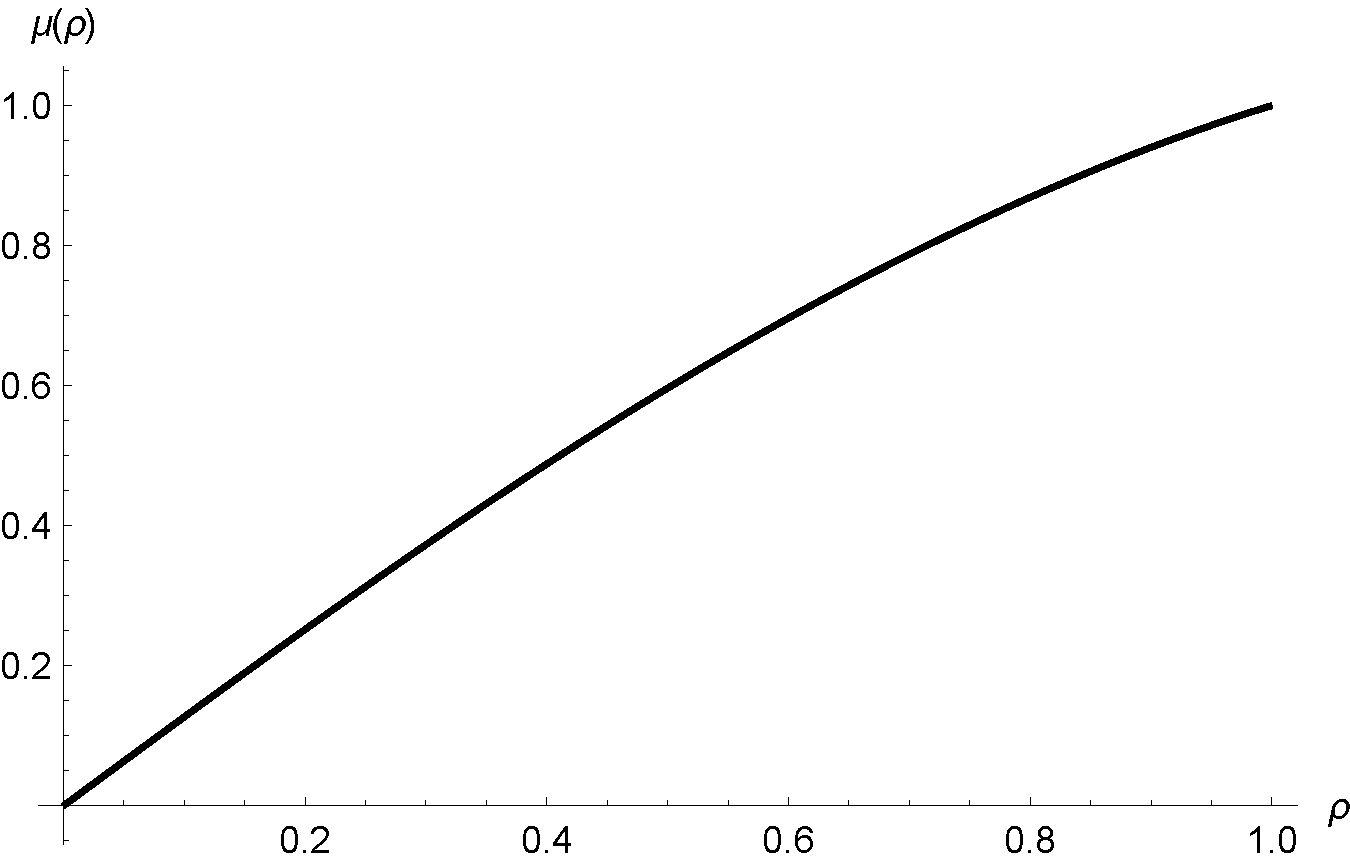
\includegraphics[width=0.6\linewidth]{ch1/mu}
    }
    \caption{Вид функции $\mu(\rho)$, при $\mu(1)=1$}
    \label{fig:ch1/mu}
\end{figure}
Вид функции $\mu(\rho)$ при другом граничном условии на правом конце может быть получен масштабированием по оси $\rho$.

\section{Построение решения}\label{sec:ch1/sec2}
\subsection{Переход от квазистатического к динамическому режиму деформирования}\label{subsec:ch1/sec2/sub1}

Рассмотрим случай $\beta=2$, который соответствует моменту перехода от квазистатического к динамическому режиму деформирования.
Положим $\text{Eu}^{-1} = C_2 \alpha^2$ и последовательно приравняем коэффициенты правых и левых частей уравнений системы \cref{eqs:ch1/sec1/substituted} при $a^{-1}$ и $\alpha^0$:
\begin{subequations}
  \label{eqs:ch1/sec2/sub1/main}
  \begin{gather}
    \label{eqs:ch1/sec2/sub1/-1/motion:2}
    -\uindex{p}{-1}_{,\xi} = 0
    \\
    \label{eqs:ch1/sec2/sub1/-1/coax:2}
    \uindex{s}{0}_{rr} \; \uindex{v}{-1}_{r,\xi} = 0
    \\
    \label{eqs:ch1/sec2/sub1/0/motion:1}
    -\uindex{p}{-1}_{,\rho}+\uindex{s}{0}_{rz,\xi} = 0
    \\
    \label{eqs:ch1/sec2/sub1/0/motion:2}
    -\uindex{p}{0}_{,\xi} - \uindex{s}{0}_{rr,\xi} - \uindex{s}{0}_{\theta\theta,\xi} = 0
    \\
    \label{eqs:ch1/sec2/sub1/0/plasticity}
    \left(\uindex{s}{0}_{rr}\right)^2 + \left(\uindex{s}{0}_{\theta\theta}\right)^2 + \uindex{s}{0}_{rr}\; \uindex{s}{0}_{\theta\theta} + \left(\uindex{s}{0}_{rz}\right)^2 = 1
    \\
    \label{eqs:ch1/sec2/sub1/0/coax:1}
    \uindex{s}{0}_{rr} \; \uindex{v}{-1}_{r} / \rho = \uindex{s}{0}_{\theta\theta} \uindex{v}{-1}_{r,\rho}
    \\
    \label{eqs:ch1/sec2/sub1/0/coax:2}
    \uindex{s}{0}_{rr} \; \uindex{v}{0}_{r,\xi} = 2 \uindex{s}{0}_{rz} \; \uindex{v}{-1}_{r,\rho}
    \\
    \label{eqs:ch1/sec2/sub1/0/uncompress}
    \uindex{v}{-1}_{r,\rho} + \uindex{v}{-1}_{r} / \rho + \uindex{v}{0}_{z,\xi} = 0
  \end{gather}
\end{subequations}
Граничные условия \cref{eq:ch1/sec1/boundary/kinematic, eq:ch1/sec1/boundary/force} при этом примут вид
\begin{equation}
  \label{eq:ch1/sec1/sub1/boundary/0}
  \uindex{v}{0}_{z}\lvert_{\xi=\pm 1} = \mp 1, \quad \lvert \uindex{s}{0}_{rz}\lvert_{\xi=\pm 1} = \mu(\rho)
\end{equation}
Из уравнений \cref{eqs:ch1/sec2/sub1/-1/motion:2, eqs:ch1/sec2/sub1/-1/coax:2} вытекает
\begin{equation*}
  \uindex{p}{-1} = \uindex{f}{-1}_{p}(\rho, \tau), \quad \uindex{v}{-1}_{r} = \uindex{f}{-1}_{v_{r}}(\rho, \tau).
\end{equation*}
Подставив выражение $\uindex{v}{-1}_{r}$ в уравнение \cref{eqs:ch1/sec2/sub1/0/uncompress} и решив дифференциальное уравнение, получим выражение для $\uindex{v}{0}_{z}$:
\begin{equation*}
  \uindex{v}{0}_{z} = \uindex{f}{0}_{v_{z}}(\rho, \tau) -\xi \left(\ \uindex{f}{-1}_{v_{r},\rho} + \uindex{f}{-1}_{v_{r}} / \rho\right)
\end{equation*}
Подстановка данного равенства в кинематические граничные условия \cref{eq:ch1/sec1/sub1/boundary/0} и использование их линейной комбинации позволяет определить неизвестные функции интегрирования:
\begin{gather*}
  \uindex{f}{0}_{v_{z}} = 0\\
  \uindex{f}{-1}_{v_{r},\rho} + \uindex{f}{-1}_{v_{r}} / \rho = 0
\end{gather*}
Окончательно получаем
\begin{gather}
  \label{sol:ch1/sec2/sub1/vr/-1}
  \uindex{v}{-1}_{r} = \uindex{f}{-1}_{v_{r}} = \rho / 2
  \\
  \label{sol:ch1/sec2/sub1/vz/0}
  \uindex{v}{0}_{z} =  -\xi
\end{gather}
Из уравнения \cref{eqs:ch1/sec2/sub1/0/motion:1} следует линейность функции $\uindex{s}{0}_{rz}$ по $\xi$, что в силу также естественно требуемой нечетности позволяет записать
\begin{equation*}
  \uindex{s}{0}_{rz} = \uindex{K}{0}_{s_{rz}}(\rho) \xi
\end{equation*}
Функцию $\uindex{K}{0}_{s_{rz}}$ определим из силовых граничных условий \cref{eq:ch1/sec1/sub1/boundary/0}:
\begin{equation*}
  \uindex{K}{0}_{s_{rz}} = -\hat{s}\mu(\rho), \quad \hat{s} = \pm1
\end{equation*}
Таким образом получаем
\begin{gather*}
  \uindex{s}{0}_{rz} = -\mu \hat{s} \xi
  \\
  \uindex{p}{-1} = \uindex{f}{-1}_{p} = \uindex{g}{-1}_{p}(\tau) - \hat{s} \int_0^\rho \mu(\zeta) d\zeta
\end{gather*}
В соответствии с физико-механическим смыслом процесса сжатия и растекания слоя сингулярная составляющая давления $\uindex{p}{-1}$ максимальна в центре слоя, то есть в окрестности $\rho = 0$ , и убывает до нуля вблизи границы $\rho=1$. Данное обстоятельство позволяет определить, что $\hat{s} = 1$ и тогда окончательно имеем
\begin{gather}
  \label{sol:ch1/sec2/sub1/srz/0}
  \uindex{s}{0}_{rz} = -\mu \xi
  \\
  \label{sol:ch1/sec2/sub1/p/-1}
  \uindex{p}{-1} = \uindex{g}{-1}_{p}(\tau) - \int_0^\rho \mu(\zeta) d\zeta = \int_\rho^1 \mu(\zeta) d\zeta + \uindex{p}{-1}_{0}(\tau)
\end{gather}
С учетом вышесказанного уравнение \cref{eqs:ch1/sec2/sub1/0/coax:1} даст равенство $\uindex{s}{0}_{rr} = \uindex{s}{0}_{\theta\theta}$ и тогда из условия пластичности \cref{eqs:ch1/sec2/sub1/0/plasticity} выразим
\begin{equation}
  \label{sol:ch1/sec2/sub1/srr+stt/0}
  \uindex{s}{0}_{rr} = \ \uindex{s}{0}_{\theta\theta} = \sqrt{\left(1-\mu^2\xi^2\right) / 3}
\end{equation}
Подставив все найденные функции в \cref{eqs:ch1/sec2/sub1/0/motion:2, eqs:ch1/sec2/sub1/0/coax:2} и решив дифференциальные уравнения найдем
\begin{equation}
  \label{sol:ch1/sec2/sub1/p+vr/0}
  \uindex{p}{0} = \uindex{f}{0}_{p}(\rho, \tau) - \frac{2}{3} \sqrt{3\left(1-\mu^2\xi^2\right)}, \quad \uindex{v}{0}_{r} = \uindex{f}{0}_{v_{r}}(\rho, \tau) + \frac{1}{\mu} \sqrt{3\left(1-\mu^2\xi^2\right)}
\end{equation}
Для нахождение неизвестных функций $\uindex{f}{0}_{p}$ и $\uindex{f}{0}_{v_{r}}$ выпишем следующее по $\alpha$ приближение уравнений \cref{eqs:ch1/sec1/substituted/motion:1, eqs:ch1/sec1/substituted/uncompress}, а также граничные условия \cref{eq:ch1/sec1/boundary/kinematic, eq:ch1/sec1/boundary/force}:
\begin{subequations}
  \begin{gather}
    \label{eqs:ch1/sec2/sub1/1/motion:1}
    -\uindex{p}{0}_{,\rho} + \uindex{s}{0}_{rr,\rho} + \uindex{s}{1}_{rz,\xi} = C_2 \left(3\rho / 4\right)
    \\
    \label{eqs:ch1/sec2/sub1/1/uncompress}
    \uindex{v}{0}_{r,\rho} + \uindex{v}{0}_{r} / \rho + \uindex{v}{1}_{z,\xi} = 0
    \\
    \label{eq:ch1/sec2/sub1/boundary/1}
    \uindex{v}{1}_{z}\lvert_{\xi=\pm 1} = 0, \quad \lvert \uindex{s}{1}_{rz}\lvert_{\xi=\pm 1} = 0
  \end{gather}
\end{subequations}
Функция $\uindex{v}{1}_{z}$ является непрерывной, поэтому имеет место равенство
\begin{equation}
  \begin{multlined}
    0 = \uindex{v}{1}_{z}\lvert_{\xi= 1} - \uindex{v}{1}_{z}\lvert_{\xi= -1} = \int_{-1}^{1}{\uindex{v}{1}_{z,\xi}d\xi} = -\int_{-1}^{1}{\left( \ \uindex{v}{0}_{r,\rho} + \uindex{v}{0}_{r} / \rho\right)d\xi} \unl{=}
    \frac{\sqrt{3}}{\mu^2 \rho}\left(\mu\sqrt{1-\mu^2} + \left(1-\frac{2\mu'}{\mu}\right)\arcsin{\mu}\right) + 2 \uindex{f}{0}_{v_{r}} / \rho + 2 \uindex{f}{0}_{v_{r},\rho}
  \end{multlined}
\end{equation}
Решая данное дифференциальное уравнение, подставив $\mu'$ из \cref{eq:ch1/sec1/mu}, получим выражение для $\uindex{f}{0}_{v_{r}}$:
\begin{equation}
  \uindex{f}{0}_{v_{r}} = \uindex{g}{0}_{v_{r}}(\tau) / \rho,
\end{equation}
причем с учетом требования конечности членов ряда, следует положить $\uindex{g}{0}_{v_{r}} = 0$.
Аналогичные операции проведем над функцией $\uindex{s}{1}_{rz}$:
\begin{gather}
  \begin{multlined}
    0 = \uindex{s}{1}_{rz}\lvert_{\xi= 1} - \uindex{s}{1}_{rz}\lvert_{\xi= -1} = \int_{-1}^{1}{\uindex{s}{1}_{rz,\xi}d\xi} = -\int_{-1}^{1}{\left( \ \uindex{p}{0}_{,\rho} - \uindex{s}{0}_{rr,\rho} + 3 C_2 \rho / 4\right)d\xi} \unl{=}
    2\left( \ \uindex{f}{0}_{p,\rho} + 3 C_2 \rho / 4\right) - \frac{d}{d\rho}\int_{-1}^{1}\uindex{s}{0}_{rr}d\xi
  \end{multlined}
  \\
  \uindex{f}{0}_{p} = -\frac{3}{8}C_2\rho^2 + \frac{1}{2}\int_{-1}^{1}\uindex{s}{0}_{rr}d\xi + \uindex{g}{0}_{p}(\tau) =
  \frac{3}{8}C_2 \left(1-\rho^2\right) + \frac{1}{2}\int_{-1}^{1}\uindex{s}{0}_{rr}d\xi + \uindex{p}{0}_{0}(\tau)
\end{gather}

\subsection{Развитый процесс динамического деформирования}\label{subsec:ch1/sec2/sub2}

Рассмотрим случай $\beta=1$, который соответствует моменту с сильным влиянием динамики в процессе сдавливания слоя.
Положим $\text{Eu}^{-1} = C_1 \alpha$ и последовательно приравняем коэффициенты правых и левых частей уравнений системы \cref{eqs:ch1/sec1/substituted} при $a^{-1}$ и $\alpha^0$:
\begin{subequations}
  \label{eqs:ch1/sec2/sub2/main}
  \begin{gather}
    \label{eqs:ch1/sec2/sub2/-1/motion:2}
    -\uindex{p}{-1}_{,\xi} = 0
    \\
    \label{eqs:ch1/sec2/sub2/-1/coax:2}
    \uindex{s}{0}_{rr} \; \uindex{v}{-1}_{r,\xi} = 0
    \\
    \label{eqs:ch1/sec2/sub2/0/motion:1}
    \begin{multlined}
      -\uindex{p}{-1}_{,\rho}+\uindex{s}{0}_{rz,\xi} = C_1 \left(
      -\frac{\rho}{2} \ \uindex{v}{-1}_{r,\rho} + \xi \ \uindex{v}{-1}_{r,\xi} + \left(1+\tau\right) \ \uindex{v}{-1}_{r,\tau} \unl[1]{+} \frac{3}{2} \ \uindex{v}{-1}_{r} + \uindex{v}{-1}_{r} \ \uindex{v}{-1}_{r,\rho} + \uindex{v}{0}_{z} \ \uindex{v}{-1}_{r,\xi}
      \right)
    \end{multlined}
    \\
    \label{eqs:ch1/sec2/sub2/0/motion:2}
    -\uindex{p}{0}_{,\xi} - \uindex{s}{0}_{rr,\xi} - \uindex{s}{0}_{\theta\theta,\xi} = 0
    \\
    \label{eqs:ch1/sec2/sub2/0/plasticity}
    \left(\uindex{s}{0}_{rr}\right)^2 + \left(\uindex{s}{0}_{\theta\theta}\right)^2 + \uindex{s}{0}_{rr}\; \uindex{s}{0}_{\theta\theta} + \left(\uindex{s}{0}_{rz}\right)^2 = 1
    \\
    \label{eqs:ch1/sec2/sub2/0/coax:1}
    \uindex{s}{0}_{rr} \; \uindex{v}{-1}_{r} / \rho = \uindex{s}{0}_{\theta\theta} \uindex{v}{-1}_{r,\rho}
    \\
    \label{eqs:ch1/sec2/sub2/0/coax:2}
    \uindex{s}{0}_{rr} \; \uindex{v}{0}_{r,\xi} = 2 \uindex{s}{0}_{rz} \; \uindex{v}{-1}_{r,\rho}
    \\
    \label{eqs:ch1/sec2/sub2/0/uncompress}
    \uindex{v}{-1}_{r,\rho} + \uindex{v}{-1}_{r} / \rho + \uindex{v}{0}_{z,\xi} = 0
  \end{gather}
\end{subequations}
Как и в предыдущем пункте граничные условия \cref{eq:ch1/sec1/boundary/kinematic, eq:ch1/sec1/boundary/force} примут вид
\begin{equation}
  \label{eq:ch1/sec1/sub2/boundary/0}
  \uindex{v}{0}_{z}\lvert_{\xi=\pm 1} = \mp 1, \quad \lvert \uindex{s}{0}_{rz}\lvert_{\xi=\pm 1} = \mu
\end{equation}
Из уравнений \cref{eqs:ch1/sec2/sub2/-1/motion:2, eqs:ch1/sec2/sub2/-1/coax:2} вытекает
\begin{equation*}
  \uindex{p}{-1} = \uindex{f}{-1}_{p}(\rho, \tau), \quad \uindex{v}{-1}_{r} = \uindex{f}{-1}_{v_{r}}(\rho, \tau).
\end{equation*}
Подставив выражение $\uindex{v}{-1}_{r}$ в уравнение \cref{eqs:ch1/sec2/sub2/0/uncompress} и решив дифференциальное уравнение, получим выражение для $\uindex{v}{0}_{z}$:
\begin{equation*}
  \uindex{v}{0}_{z} = \uindex{f}{0}_{v_{z}}(\rho, \tau) -\xi \left(\ \uindex{f}{-1}_{v_{r},\rho} + \uindex{f}{-1}_{v_{r}} / \rho\right)
\end{equation*}
Подстановка данного равенства в кинематические граничные условия \cref{eq:ch1/sec1/sub2/boundary/0} и использование их линейной комбинации позволяет определить неизвестные функции интегрирования:
\begin{gather*}
  \uindex{f}{0}_{v_{z}} = 0
  \\
  \uindex{f}{-1}_{v_{r},\rho} + \uindex{f}{-1}_{v_{r}} / \rho = 0
\end{gather*}
Окончательно получаем
\begin{gather}
  \label{sol:ch1/sec2/sub2/vr/-1}
  \uindex{v}{-1}_{r} = \uindex{f}{-1}_{v_{r}} = \rho / 2
  \\
  \label{sol:ch1/sec2/sub2/vz/0}
  \uindex{v}{0}_{z} =  -\xi
\end{gather}
С учетом \cref{sol:ch1/sec2/sub2/vr/-1} уравнение \cref{eqs:ch1/sec2/sub2/0/motion:1} примет вид
\begin{equation*}
  -\uindex{p}{-1}_{,\rho}+\uindex{s}{0}_{rz,\xi} = C_1 \left(3 \rho / 4\right)
\end{equation*}
Решая его относительно $\uindex{s}{0}_{rz}$ и используя силовые граничные условия \cref{eq:ch1/sec1/sub2/boundary/0} придем к
\begin{gather*}
  \uindex{s}{0}_{rz} = 3 C_1 \xi \rho / 4 + \xi \uindex{f}{-1}_{p,\rho} + \uindex{f}{0}_{s_{rz}}(\rho, \tau)
  \\
  \uindex{f}{0}_{s_{rz}} = 0
  \\
  3 C_1 \rho / 4 + \uindex{f}{-1}_{p,\rho} = -2 \mu \hat{s}, \quad \hat{s} = \pm 1
  \\
  \uindex{p}{-1} = \uindex{f}{-1}_{p} = - \frac{3}{8}C_1\rho^2 + \uindex{g}{-1}_{p}(\tau) - \hat{s} \int_0^\rho \mu(\zeta)d\zeta
\end{gather*}
В силу тех же рассуждений, что приводились в \ref{subsec:ch1/sec2/sub1} следует положить $\hat{s} = 1$. Тогда найденные функции можно записать в следующем виде:
\begin{gather}
  \label{sol:ch1/sec2/sub2/srz/0}
  \uindex{s}{0}_{rz} = -\mu \xi
  \\
  \label{sol:ch1/sec2/sub2/p/-1}
  \uindex{p}{-1} = - \frac{3}{8}C_1\rho^2 + \uindex{g}{-1}_{p}(\tau) - \int_0^\rho \mu(\zeta)d\zeta = \frac{3}{8}C_1\left(1-\rho^2\right) + \int_\rho^1 \mu(\zeta)d\zeta + \uindex{p}{-1}_{0}(\tau)
\end{gather}
С учетом вышесказанного уравнение \cref{eqs:ch1/sec2/sub2/0/coax:1} даст равенство $\uindex{s}{0}_{rr} = \uindex{s}{0}_{\theta\theta}$ и тогда из условия пластичности \cref{eqs:ch1/sec2/sub2/0/plasticity} выразим
\begin{equation}
  \label{sol:ch1/sec2/sub2/srr+stt/0}
  \uindex{s}{0}_{rr} = \ \uindex{s}{0}_{\theta\theta} = \sqrt{\left(1-\mu^2\xi^2\right) / 3}
\end{equation}
Подставив все найденные функции в \cref{eqs:ch1/sec2/sub2/0/motion:2, eqs:ch1/sec2/sub2/0/coax:2} и решив дифференциальные уравнения найдем
\begin{equation}
  \label{sol:ch1/sec2/sub2/p+vr/0}
  \uindex{p}{0} = \uindex{f}{0}_{p}(\rho, \tau) - \frac{2}{3} \sqrt{3\left(1-\mu^2\xi^2\right)}, \quad \uindex{v}{0}_{r} = \uindex{f}{0}_{v_{r}}(\rho, \tau) + \frac{1}{\mu} \sqrt{3\left(1-\mu^2\xi^2\right)}
\end{equation}
Для нахождение неизвестных функций $\uindex{f}{0}_{p}$ и $\uindex{f}{0}_{v_{r}}$ выпишем следующее по $\alpha$ приближение уравнений \cref{eqs:ch1/sec1/substituted/motion:1, eqs:ch1/sec1/substituted/uncompress}, а также граничные условия \cref{eq:ch1/sec1/boundary/kinematic, eq:ch1/sec1/boundary/force}:
\begin{subequations}
  \begin{gather}
    \label{eqs:ch1/sec2/sub2/1/motion:1}
    -\uindex{p}{0}_{,\rho}+\uindex{s}{0}_{rr,\rho}+\uindex{s}{1}_{rz,\xi} = C_1 \left(\ \uindex{v}{0}_{r} / 2 + \left(1+\tau\right)\uindex{v}{0}_{r,\tau}\right)
    \\
    \label{eqs:ch1/sec2/sub2/1/uncompress}
    \uindex{v}{0}_{r,\rho} + \uindex{v}{0}_{r} / \rho + \uindex{v}{1}_{z,\xi} = 0
    \\
    \label{eq:ch1/sec2/sub2/boundary/1}
    \uindex{v}{1}_{z}\lvert_{\xi=\pm 1} = 0, \quad \lvert \uindex{s}{1}_{rz}\lvert_{\xi=\pm 1} = 0
  \end{gather}
\end{subequations}
Функция $\uindex{v}{1}_{z}$ является непрерывной, поэтому имеет место равенство
\begin{equation}
  \begin{multlined}
    0 = \uindex{v}{1}_{z}\lvert_{\xi= 1} - \uindex{v}{1}_{z}\lvert_{\xi= -1} = \int_{-1}^{1}{\uindex{v}{1}_{z,\xi}d\xi} = -\int_{-1}^{1}{\left( \ \uindex{v}{0}_{r,\rho} + \uindex{v}{0}_{r} / \rho\right)d\xi} \unl{=}
    \frac{\sqrt{3}}{\mu^2 \rho}\left(\mu\sqrt{1-\mu^2} + \left(1-\frac{2\mu'}{\mu}\right)\arcsin{\mu}\right) + 2 \uindex{f}{0}_{v_{r}} / \rho + 2 \uindex{f}{0}_{v_{r},\rho}
  \end{multlined}
\end{equation}
Решая данное дифференциальное уравнение, подставив $\mu'$ из \cref{eq:ch1/sec1/mu}, получим выражение для $\uindex{f}{0}_{v_{r}}$:
\begin{equation}
  \uindex{f}{0}_{v_{r}} = \uindex{g}{0}_{v_{r}}(\tau) / \rho,
\end{equation}
причем с учетом требования конечности членов ряда, следует положить $\uindex{g}{0}_{v_{r}} = 0$.
Аналогичные операции проведем над функцией $\uindex{s}{1}_{rz}$:
\begin{gather}
  \begin{multlined}
    0 = \uindex{s}{1}_{rz}\lvert_{\xi= 1} - \uindex{s}{1}_{rz}\lvert_{\xi= -1} = \int_{-1}^{1}{\uindex{s}{1}_{rz,\xi}d\xi} = -\int_{-1}^{1}{\left( \ \uindex{p}{0}_{,\rho} - \uindex{s}{0}_{rr,\rho} + C_1 \uindex{v}{0}_{r} / 2\right)d\xi} \unl{=}
    2 \uindex{f}{0}_{p,\rho} + C_1 \int_{-1}^{1} \uindex{v}{0}_{r} d\xi  - \frac{d}{d\rho}\int_{-1}^{1}\uindex{s}{0}_{rr}d\xi
  \end{multlined}
  \\
  \uindex{f}{0}_{p} = -C_1 \int\left(\int_{-1}^{1} \uindex{v}{0}_{r} d\xi\right) d\rho + \frac{1}{2}\int_{-1}^{1}\uindex{s}{0}_{rr}d\xi + \uindex{g}{0}_{p}(\tau)
\end{gather}
Выражение $\int\left(\int_{-1}^{1} \uindex{v}{0}_{r} d\xi\right) d\rho$ может быть вычисленно только при задании функции $\mu(\rho)$. Однако возможно упрощение данного выражения:
\begin{gather*}
  \int_{-1}^{1} \uindex{v}{0}_{r} d\xi = \frac{\sqrt{3}\arcsin\mu}{\mu^2}\left(1+\frac{\mu\sqrt{1-\mu^2}}{\arcsin\mu}\right) = \frac{\sqrt{3}\arcsin\mu}{\mu^2} \frac{2\rho}{\mu}\mu' = f(\rho)
  \\
  \int f d\rho = \int\frac{\sqrt{3}\arcsin\mu}{\mu^2} \frac{2\rho}{\mu}d\mu = -\int \rho d\frac{\sqrt{3}\arcsin\mu}{\mu^2}\left(1+\frac{\mu\sqrt{1-\mu^2}}{\arcsin\mu}\right)
  \\
  \int f d\rho + \int \rho d f = \int(f \frac{d\rho}{d\rho} + \frac{d f}{d\rho}\rho)d\rho = \int \frac{d}{d\rho}\left(f \rho\right) d\rho = 0
  \\
  \frac{d}{d\rho}\left(f \rho\right) = 0 \Rightarrow f \rho = \uindex{C}{0}_{p} \Rightarrow f = \uindex{C}{0}_{p} / \rho, \quad \uindex{C}{0}_{p} = \const
  \\
  \int f d\rho = \int \frac{c}{\rho} d\rho = \uindex{C}{0}_{p} \log \rho,
\end{gather*}
где константа $\uindex{C}{0}_{p}$ определяется по функции $\mu$. Тогда выражение $\uindex{f}{0}_{p}$ можно периписать в виде
\begin{equation}
  \uindex{f}{0}_{p} = C_1 \left(1- \uindex{C}{0}_{p} \log\rho\right) + \frac{1}{2}\int_{-1}^{1}\uindex{s}{0}_{rr}d\xi + \uindex{p}{0}_{0}(\tau)
\end{equation}

\section{Анализ решения}\label{sec:ch1/sec3}

Полученные решения \cref{sol:ch1/sec2/sub1/p/-1,sol:ch1/sec2/sub1/srz/0,sol:ch1/sec2/sub1/vr/-1,sol:ch1/sec2/sub1/vz/0,sol:ch1/sec2/sub1/srr+stt/0,sol:ch1/sec2/sub1/vz/0,sol:ch1/sec2/sub1/p+vr/0} и \cref{sol:ch1/sec2/sub2/p/-1,sol:ch1/sec2/sub2/srz/0,sol:ch1/sec2/sub2/vr/-1,sol:ch1/sec2/sub2/vz/0,sol:ch1/sec2/sub2/srr+stt/0,sol:ch1/sec2/sub2/vz/0,sol:ch1/sec2/sub2/p+vr/0} являются приближенными и с точностью $O(\alpha)$ совпадают, за исключением функции давления, с квазистатическим решением \autocite{Georgievsky:2008}:
\begin{subequations}
  \begin{gather}
    \label{sol:ch1/sec3/p/qs}
    p = p_0 + \frac{\tau_{s}}{\alpha}\int_\rho^1 \mu(\zeta) d\zeta + \frac{1}{2}\int_{-1}^{1}s_{rr}d\xi - \frac{2\tau_{s}}{\sqrt{3}} \sqrt{\left(1-\mu^2\xi^2\right)} + O(\alpha)
    \\
    s_{rr} = s_{\theta\theta} = \tau_{s} \sqrt{\left(1-\mu^2\xi^2\right) / 3} + O(\alpha)
    \\
    s_{rz} = - \mu \xi \tau_{s}  + O(\alpha)
    \\
    v_{r} / V = \frac{\rho}{2\alpha} + \frac{1}{\mu} \sqrt{3\left(1-\mu^2\xi^2\right)} + O(\alpha)
    \\
    v_{z}= - V \xi  + O(\alpha)
  \end{gather}
\end{subequations}
где $p_0$ имеет смысл гидростатического давления. Обозначим правую часть уравнения \cref{sol:ch1/sec3/p/qs} как $p^\text{кв}$. Для случаев $\beta=2$ и $\beta=1$ имеем соответственно:
\begin{gather}
  \left(p\lvert_{\beta=2}\right) = p^\text{кв} + \frac{3\tau_{s}}{8}C_2 \left(1-\rho^2\right)
  \\
  \left(p\lvert_{\beta=1}\right) = p^\text{кв} + \frac{3\tau_{s}}{8\alpha}C_1 \left(1-\rho^2\right) + C_1 \left(1- \uindex{C}{0}_{p} \log\rho\right) \tau_{s}
\end{gather}
При сравнении выражений видно, что в случае динамического сдавливания возникает квадратично зависящее от радиуса слагаемое, причем, чем динамичнее происходит процесс, тем более значима становится данная величина. Наличие такой зависимости качественно меняет эпюру давления в слое и увеличивает суммарную силу, действующую со стороны слоя на плиты.



Используя то, что $\alpha(t) = \left(V \left(t_*-t\right)\right)^{3/2} \sqrt{2\pi / \mathcal{V}_0}$, где $\mathcal{V}_0$ -- объем слоя, можно установить зависимость между временем и стадией прессования:
\begin{equation}
  t_* - t \sim \frac{\text{Eu}^{\nicefrac{-2}{3\beta}}}{V}\sqrt[3]{\frac{\mathcal{V}_0}{2\pi}}
\end{equation}
           % Глава 1
\chapter{Задача о сдавливании цилиндрического идеально жесткопластического слоя}\label{ch:ch2}
Известное решение Прандтля \autocite{Prandtl:1948} о сжатии тонкой полосы примечательно тем, что является отправной точкой для построение математических моделей, имеющих непосредственное отношение к технологическим процессам обработки металлов давлением. Одним из обобщений данного решения на случай слоя конечного объема является задача о сдавливании цилиндрического слоя \autocite{Georgievsky:2010}. Её решение находит применение в технологических процессах изготовления тонкостенного трубопровода заданной точности. В отличие от классической задачи Прандтля, случай цилиндрического слоя дополнительно параметризуется отношением радиусов прессующих цилиндров к длине образующей. В данной постановке задачи исследуется влияние динамических эффектов в процессе формирования изделия методом прессования. Материалы главы содержатся в публикации \autocite{Shabaykin:2020b}.

\section{Постановка задачи и асимптотические разложения}\label{sec:ch2/sec1}

Пренебрегая начальными упругими деформациями, вязкостью и незначительным упрочнением, материал, имеющий плотность $\varrho$, полагается несжимаемым идеально жесткопластическим, удовлетворяющим тензорно линейным определяющим соотношениям и скалярному определяющему соотношению -- квадратичному критерию Мизеса-Генки $\sigma_{u} = \sigma_{s}$, где $\sigma_{u} = \sqrt{\utilde{s} : \utilde{s}}$ -- интенсивность напряжения, $\utilde{s}$ -- девиатор напряжения, $\sigma_{s}$ -- предел текучести.

Пусть течение происходит в области
\begin{equation}
  \Omega_{t} = \{0 \le r \le R(t) + h(t), -l(t) \le z \le l(t), 0 \le \theta < 2\pi\},
\end{equation}
с границей $\partial\Omega = \Gamma = \Gamma_{1} \cup \Gamma_{2} \cup \Gamma_{3}\cup \Gamma_{4}$, причем $h(t) \ll l(t)$ для любого $t \ge 0$. В начальный момент времени область, занятая материалом, имела вид
\begin{equation}
  \Omega_{0} = \{0 \le r \le R_{0} + h_{0}, -l_{0} \le z \le l_{0}, 0 \le \theta < 2\pi\}, \quad \partial\Omega_{0} = \Gamma_{0}
\end{equation}
поэтому в силу несжимаемости $(2R+h)hl=(2R_{0}+h_{0})h_{0}l_{0}$.

\begin{figure}[ht]
  \centerfloat{
    \includegraphics[width=0.6\linewidth]{./ch2/layer}
    }
    \caption{Представление цилиндрического слоя}
    \label{fig:ch2/layer}
\end{figure}
Скорость расширения внутреннего цилиндра обозначим $V$, поэтому кинематическое условие непротекания сквозь границы $\Gamma_{1}$ и $\Gamma_{2}$ имеет вид
\begin{equation}
  \label{eq:ch2/sec1/boundary/kinematic}
  v_{r}\lvert_{r=R} = V, \quad v_{r}\lvert_{r=R+h} = 0
\end{equation}
Касательная составляющая скорости (в данном случае $v_{z}$) на указанных границах идеальной среды, как известно, не задаётся.

В некоторый момент времени $0 < t < h_{0}/V = t_*$, где $t_*$ -- момент схлопывания слоя, относительно шести функций -- независимых компонент девиатора напряжений $s_{rr}$, $s_{rz}$ и $s_{\theta\theta}$, давления $p$ и компонент скорости $v_{r}$ и $v_{z}$ -- должна выполнятся замкнутая система уравнений динамической теории идеальной пластичности для цилиндрических координат:
\begin{subequations}
  \label{eqs:ch2/sec1/general}
  \begin{gather}
    \label{eqs:ch2/sec1/general/motion:1}
    -p_{,r}+s_{rr,r}+s_{rz,z}+\frac{s_{rr}-s_{\theta\theta}}{r} = \varrho \left(v_{r;t}+v_{r} v_{r,r} + v_{z} v_{r,z} \right)
    \\
    \label{eqs:ch2/sec1/general/motion:2}
    -p_{,z}+s_{rz,r}+\frac{s_{rz}}{r}-(s_{rr}+s_{\theta\theta})_{,z} = \varrho \left(v_{z;t}+v_{r} v_{z,r} + v_{z} v_{z,z} \right)
    \\
    \label{eqs:ch2/sec1/general/plasticity}
    s^2_{rr}+s^2_{\theta\theta}+s_{rr} s_{\theta\theta} + s^2_{rz}=\tau^2_{s}
    \\
    \label{eqs:ch2/sec1/general/coax:1}
    s_{rr} \frac{v_{r}}{r} = s_{\theta\theta} v_{r,r}
    \\
    \label{eqs:ch2/sec1/general/coax:2}
    s_{rr} (v_{r,z}+v_{z,r}) = 2 s_{rz} v_{r,r}
    \\
    \label{eqs:ch2/sec1/general/uncompress}
    v_{r,r}+\frac{v_{r}}{r}+v_{z,z} = 0
  \end{gather}
\end{subequations}
Кроме выполнения условия \cref{eq:ch2/sec1/boundary/kinematic} на жестких контактирующих поверхностях потребуем, что бы модуль касательного напряжения $s_{rz}$ достигал на границах $\Gamma_{1}$ и $\Gamma_{2}$ своего максимального значения:
\begin{equation}
  \label{eq:ch2/sec1/boundary/force}
  \lvert s_{rz}\lvert_{r=R} = \lvert s_{rz}\lvert_{r=R+h} = \mu \tau_{s}, \quad 0 < \mu \le 1,
\end{equation}
где $\mu$ -- шероховатость пресса. Абсолютной шероховатости, или полному сцеплению пресса с материалом, соответствует значение $\mu = 1$.

В реальном процессе сжатия слоя границы $\Gamma_{3}$ и $\Gamma_{4}$, естественно, свободны от напряжений, однако в математической постановке рассматриваемой здесь краевой задачи в её классическом варианте данное условие не ставится. Поэтому других, помимо \cref{eq:ch2/sec1/boundary/kinematic, eq:ch2/sec1/boundary/force}, граничных условий в задаче не предполагается, а область вблизи границ $\Gamma_{3}$ и $\Gamma_{4}$(на расстояниях порядка $h$) трактуется как зона краевого эффекта.

Введем малый параметр $\alpha = \frac{h(t)}{l(t)} \ll 1$ и проведем разложение всех неизвестных величин, входящих в систему уравнений \cref{eqs:ch2/sec1/general}, в ряды по целым степеням параметра:
\begin{subequations}
  \label{eqs:ch2/series}
  \begin{gather}
    v_{r}\left(r, z, t\right) = V \sum_{k=0}^{\infty}{\alpha^{k} \; \uindex{v}{k}_{r}}
    \\
    v_{z}\left(r, z, t\right) = V \sum_{k=-N}^{\infty}{\alpha^{k} \; \uindex{v}{k}_{z}}, \quad N \ge 1
    \\
    s_{ij}\left(r, z, t\right) = \tau_{s} \sum_{k=0}^{\infty}{\alpha^{k} \; \uindex{s}{k}_{ij}}, \quad (ij)\in\{rr, rz, \theta\theta\}
    \\
    p\left(r, z, t \right) = \tau_{s} \sum_{k=-M}^{\infty}{\alpha^{k} \; \uindex{p}{k}}, \quad M \ge 1
  \end{gather}
\end{subequations}
Коэффициенты рядов \cref{eqs:ch2/series} -- безразмерны и являются функциями безразмерных координат $\rho, \xi, \tau$ :
\begin{equation}
  \label{eq:ch2/coordinates}
  \rho = \frac{r-R}{h}, \quad \xi = \frac{z}{l}=\frac{\alpha z}{h}, \quad \tau = V \frac{t}{h}
\end{equation}
Наличие в \cref{eqs:ch2/series} членов $\alpha^{-n} \; \uindex{v}{-n}_{z}$ и $\alpha^{-m} \; \uindex{p}{-m}$ обусловлено стремлением $v_{r}$ и $p$ к бесконечности, при $\alpha\rightarrow 0$, что ясно из физических соображений. Также заметим, что область $\Omega$ содержит три геометрических размера: $h$, $l$ И $R$, и если отношеные первых двух образую малый параметр, то отнощшение двух последних может иметь любой ``промежуточный'' порядок малости:
\begin{equation}
  \label{eq:ch2/sec1/c}
  R/l = a \alpha^c, \quad c\in[0,1], \quad a=O(1)
\end{equation}
Обратимся к геометрическому условию несжимаемости и выразим малый параметр и координаты \cref{eq:ch2/coordinates} как эволюционные функции:
\begin{subequations}
  \begin{gather}
    \left(\left(2r+h\right)h l\right)^. = 0, \quad \dot{l} = \frac{2 V R l}{\left(2R + h\right)h}=\frac{2 V R/l}{\left(2R/l + \alpha\right)\alpha}=\frac{2 V a \alpha^c}{\left(2a \alpha^c + \alpha\right)\alpha}\nonumber
    \\
    \dot{\alpha} = \left(\frac{h}{l}\right)^. = \frac{\dot{h}l - h\dot{l}}{l^2} = -\frac{V\alpha}{h}\left(2-\frac{\alpha}{2a\alpha^c+\alpha}\right)
    \\
    \dot{\rho} = \left(\frac{r-R}{h}\right)^. = \frac{-\dot{R} h - \dot{h}\left(r-R\right)}{h^2} = \frac{V}{h}\left(\rho-1\right)
    \\
    \dot{\xi} = \left(\frac{z}{l}\right)^. = -\frac{z \dot{l}}{l^2} = -\frac{V\xi\alpha}{h}\left(1-\frac{\alpha}{2a\alpha^c+\alpha}\right)
    \\
    \dot{\tau} = \left(V \frac{t}{h}\right)^. = V \frac{h - t\dot{h}}{h^2} = \frac{V}{h} \left(1+\tau\right)
  \end{gather}
\end{subequations}
Подставляя выражения \cref{eqs:ch2/series} в систему \cref{eqs:ch2/sec1/general} и учитывая, что полная производная по времени представляется в виде
\begin{equation*}
  \uindex{v}{k}_{i;t} = \uindex{v}{k}_{i,\rho} \dot{\rho} + \uindex{v}{k}_{i,\xi} \dot{\xi} + \uindex{v}{k}_{i,\tau} \dot{\tau}
\end{equation*}
получим следующую систему:
\begingroup
\allowdisplaybreaks
\begin{subequations}
  \label{eqs:ch2/sec1/substituted}
  \begin{gather}
    \label{eqs:ch2/sec1/substituted/motion:1}
    \begin{multlined}
      -\sum_{k=-M}^{\infty}{\alpha^{k} \; \uindex{p}{k}_{,\rho}} + \sum_{k=0}^{\infty}{\alpha^{k}\left(
      \ \uindex{s}{k}_{rr,\rho} + \alpha \ \uindex{s}{k}_{rz,\xi} + \frac{\alpha}{\alpha\rho+a \alpha^c}\left(\ \uindex{s}{k}_{rr} - \uindex{s}{k}_{\theta\theta}\right)
      \right)} \unl{=} \frac{\varrho V^2}{\tau_{s}}\left(
      \sum_{k=0}^{\infty}\alpha^{k}\left(
      \uindex{v}{k}_{r,\rho} \left(\rho+1\right) -
      \uindex{v}{k}_{r,\xi} \xi\alpha\left(1-\frac{\alpha}{2a\alpha^c+\alpha}\right) \right. \unl[1]{+} \uindex{v}{k}_{r,\tau} \left(1+\tau\right) -
      \left(2-\frac{\alpha}{2a\alpha^c+\alpha}\right) \ \uindex{v}{k}_{r}
      \right) \unl{+}
      \left.
      \sum_{k=0}^{\infty}{\alpha^{k} \; \uindex{v}{k}_{r}} \sum_{k=0}^{\infty}{\alpha^{k} \; \uindex{v}{k}_{r,\rho}} +
      \sum_{k=-N}^{\infty}{\alpha^{k} \; \uindex{v}{k}_{z}} \sum_{k=0}^{\infty}{\alpha^{k+1} \; \uindex{v}{k}_{r,\xi}}
      \right)
    \end{multlined}
    \\
    \label{eqs:ch2/sec1/substituted/motion:2}
    \begin{multlined}
      -\sum_{k=-M}^{\infty}{\!\!\alpha^{k+1} \ \uindex{p}{k}_{,\xi}} \!+\!
      \sum_{k=0}^{\infty}{\alpha^{k}\!\left(
      \uindex{s}{k}_{rz,\rho} +
      \frac{\alpha}{\alpha\rho+a \alpha^c} \ \uindex{s}{k}_{rz} -
      \alpha\left(\ \uindex{s}{k}_{rr,\xi} + \uindex{s}{k}_{\theta\theta,\xi}\right)
      \right)} \unl{=}
      \frac{\varrho V^2}{\tau_{s}}\left(
      \sum_{k=-N}^{\infty}\alpha^{k}\left(
      \uindex{v}{k}_{z,\rho} \left(\rho+1\right) -
      \uindex{v}{k}_{z,\xi} \xi\alpha\left(1-\frac{\alpha}{2a\alpha^c+\alpha}\right) \right. \unl[1]{+} \uindex{v}{k}_{z,\tau} \left(1+\tau\right) -
      \left(2-\frac{\alpha}{2a\alpha^c+\alpha}\right) \ \uindex{v}{k}_{z}
      \right) \unl{+}
      \left.
      \sum_{k=0}^{\infty}{\alpha^{k} \; \uindex{v}{k}_{r}} \sum_{k=-N}^{\infty}{\alpha^{k} \; \uindex{v}{k}_{z,\rho}} +
      \sum_{k=-N}^{\infty}{\alpha^{k} \; \uindex{v}{k}_{z}} \sum_{k=-N}^{\infty}{\alpha^{k+1} \; \uindex{v}{k}_{z,\xi}}
      \right)
    \end{multlined}
    \\
    \label{eqs:ch2/sec1/substituted/plasticity}
    \begin{multlined}
      \left(\sum_{k=0}^{\infty}{\alpha^{k} \; \uindex{s}{k}_{rr}}\right)^2+
      \left(\sum_{k=0}^{\infty}{\alpha^{k} \; \uindex{s}{k}_{\theta\theta}}\right)\unl{+}
      \sum_{k=0}^{\infty}{\alpha^{k} \; \uindex{s}{k}_{rr}} \sum_{k=0}^{\infty}{\alpha^{k} \; \uindex{s}{k}_{\theta\theta}}+
      \left(\sum_{k=0}^{\infty}{\alpha^{k} \; \uindex{s}{k}_{rz}}\right)^2 = 1
    \end{multlined}
    \\
    \label{eqs:ch2/sec1/substituted/coax:1}
    \sum_{k=0}^{\infty}{\alpha^{k} \; \uindex{s}{k}_{rr}} \; \frac{\alpha}{\alpha\rho+a \alpha^c} \sum_{k=0}^{\infty}{\alpha^{k} \; \uindex{v}{k}_{r}} = \sum_{k=0}^{\infty}{\alpha^{k} \; \uindex{s}{k}_{\theta\theta}} \sum_{k=0}^{\infty}{\alpha^{k} \; \uindex{v}{k}_{r,\rho}}
    \\
    \label{eqs:ch2/sec1/substituted/coax:2}
    \sum_{k=0}^{\infty}{\alpha^{k} \; \uindex{s}{k}_{rr}} \left(
    \sum_{k=0}^{\infty}{\alpha^{k+1} \; \uindex{v}{k}_{r,\xi}} +
    \sum_{k=-N}^{\infty}{\alpha^{k} \; \uindex{v}{k}_{z,\rho}}
    \right) = 2 \sum_{k=0}^{\infty}{\alpha^{k} \; \uindex{s}{k}_{rz}} \sum_{k=0}^{\infty}{\alpha^{k} \; \uindex{v}{k}_{r,\rho}}
    \\
    \label{eqs:ch2/sec1/substituted/uncompress}
    \sum_{k=0}^{\infty}{\alpha^{k} \; \uindex{v}{k}_{r,\rho}} + \frac{\alpha}{\alpha\rho+a \alpha^c}\sum_{k=0}^{\infty}{\alpha^{k} \; \uindex{v}{k}_{r}} + \sum_{k=-N}^{\infty}{\alpha^{k+1} \; \uindex{v}{k}_{z,\xi}} = 0
  \end{gather}
\end{subequations}
\endgroup
Возникший в правой части уравнений \cref{eqs:ch2/sec1/substituted/motion:1, eqs:ch2/sec1/substituted/motion:2} коэффициент равен обратному числу Эйлера
\begin{equation*}
  \text{Eu}^{-1} = \frac{\varrho V^2}{\tau_{s}}.
\end{equation*}
Данная величина мала \todo{почему?}и как видно из её определения фиксирована. По сравнению с ней порядок малости $\alpha(t)$ при течении времени от 0 до $t_*$ растёт до бесконечности. Это позволяет записать
\begin{equation*}
  \text{Eu}^{-1} = O\left(\alpha^\beta(t)\right), \text{ причем } \beta \rightarrow 0 \text{ при } t \rightarrow t_*
\end{equation*}
Применительно к динамическому анализу интерес представляет $0 < \beta \le 2$. Отыскание решений проведем для целочисленных значений входящих в этот диапазон.

Обратимся к системе двух последних уравнений \cref{eqs:ch2/sec1/substituted/coax:2, eqs:ch2/sec1/substituted/uncompress}. Из них сразу следует, что $\uindex{v}{-N}_{r,\xi} = 0$ и $\uindex{v}{-N}_{r,\rho} = 0$, то есть $\uindex{v}{-N}_{z} = \uindex{g}{-N}_{v_{z}}(\tau)$ зависит только от $\tau$, обуславливая перемещение вдоль оси $z$ как абсолютно жесткого целого. Исключив данное движение из рассмотрения, можно принять $\uindex{v}{-N}_{z} = 0$. Аналогичные рассуждения применимы последовательно для $\uindex{v}{-N+1}_{z}$, затем $\uindex{v}{-N+2}_{z}$ и далее вплоть до $\uindex{v}{-2}_{z}$.
Учитывая, что первый ненулевой член продольной компоненты скорости $\uindex{v}{-1}_{z}$, и принимая, что $\beta \ge 1$ определим из уравнений \cref{eqs:ch2/sec1/substituted/motion:1, eqs:ch2/sec1/substituted/motion:2} порядок малости для функции давления $p$. Для $M \ge 2$ имеем:
\begin{equation*}
  -\uindex{p}{-M}_{,\rho} = 0, \quad -\uindex{p}{-M}_{,\xi} = 0 \text{ и, следовательно, } \ \uindex{p}{-M} = \uindex{p}{-M}_{0}(\tau)
\end{equation*}
Здесь $\uindex{p}{-M}_{0}$ -- гидростатическая постоянная, не дающая вклад в уравнение движения и однозначно определяемая заданием внешнего давления. Поэтому, без ограничения общности, можно считать, что $M=1$.

В указанном в \cref{eq:ch2/sec1/c} диапазоне параметра $c$ выделим три значения, соответствующие различным математическим и механическим смыслам:
\begin{itemize}
  \item $c=1$, когда радиусы цилиндров имеют порядок толщины слоя,
  \item $c=0$, когда радиусы цилиндров имеют порядок длины образующей,
  \item $0<c<1$, когда радиусы цилиндров имеют ``промежуточный'' порядок малости.
\end{itemize}
\section{Построение решения при радиусах цилиндров порядка толщины слоя}\label{sec:ch2/sec2}

При данном соотношении дробь $\frac{\alpha}{\alpha\rho+a \alpha^c}$ преобразуется к виду $\frac{1}{\rho+a}$ и не будет зависеть от $\alpha$, следовательно, будет являться величиной порядка $O(1)$.

\subsection{Переход от квазистатического к динамическому режиму деформирования}\label{subsec:ch2/sec2/sub1}

Рассмотрим случай $\beta=2$, который соответствует моменту перехода от квазистатического к динамическому режиму деформирования.

Положим $\text{Eu}^{-1} = C_2 \alpha^2$ и последовательно приравняем коэффициенты правых и левых частей уравнений системы \cref{eqs:ch2/sec1/substituted} при $a^{-1}$ и $\alpha^0$:
\begingroup
\allowdisplaybreaks
\begin{subequations}
  \label{eqs:ch2/sec2/sub1/main}
  \begin{gather}
    \label{eqs:ch2/sec2/sub1/-1/motion:2}
    -\uindex{p}{-1}_{,\rho} = 0
    \\
    \label{eqs:ch2/sec2/sub1/-1/coax:2}
    \uindex{s}{0}_{rr} \; \uindex{v}{-1}_{z,\rho} = 0
    \\
    \label{eqs:ch2/sec2/sub1/0/motion:1}
    -\uindex{p}{0}_{,\rho}+\uindex{s}{0}_{rr,\rho} + \left(\uindex{s}{0}_{rr}-\uindex{s}{0}_{\theta\theta}\right) / \left(\rho + a\right) = 0
    \\
    \label{eqs:ch2/sec2/sub1/0/motion:2}
    -\uindex{p}{-1}_{,\xi} + \uindex{s}{0}_{rz,\rho} + \uindex{s}{0}_{rz} / \left(\rho+a\right) = 0
    \\
    \label{eqs:ch2/sec2/sub1/0/plasticity}
    \left(\uindex{s}{0}_{rr}\right)^2 + \left(\uindex{s}{0}_{\theta\theta}\right)^2 + \uindex{s}{0}_{rr}\; \uindex{s}{0}_{\theta\theta} + \left(\uindex{s}{0}_{rz}\right)^2 = 1
    \\
    \label{eqs:ch2/sec2/sub1/0/coax:1}
    \uindex{s}{0}_{rr} \; \uindex{v}{0}_{r} / \left(\rho+a\right) = \uindex{s}{0}_{\theta\theta} \uindex{v}{0}_{r,\rho}
    \\
    \label{eqs:ch2/sec2/sub1/0/coax:2}
    \uindex{s}{0}_{rr} \; \uindex{v}{0}_{z,\rho} = 2 \uindex{s}{0}_{rz} \; \uindex{v}{0}_{r,\rho}
    \\
    \label{eqs:ch2/sec2/sub1/0/uncompress}
    \uindex{v}{0}_{r,\rho} + \uindex{v}{0}_{r} / \left(\rho+a\right) + \uindex{v}{-1}_{z,\xi} = 0
  \end{gather}
\end{subequations}
\endgroup
Граничные условия \cref{eq:ch2/sec1/boundary/kinematic, eq:ch2/sec1/boundary/force} при этом примут вид
\begin{equation}
  \label{eq:ch2/sec2/sub1/boundary/0}
  \uindex{v}{0}_{r}\lvert_{\rho=0} = 1,\quad \uindex{v}{0}_{r}\lvert_{\rho=1} = 0, \quad \lvert \uindex{s}{0}_{rz}\lvert_{\rho=0} = \lvert \uindex{s}{0}_{rz}\lvert_{\rho=1} = \mu
\end{equation}
Из уравнений \cref{eqs:ch2/sec2/sub1/-1/motion:2, eqs:ch2/sec2/sub1/-1/coax:2} вытекает
\begin{equation*}
  \uindex{p}{-1} = \uindex{f}{-1}_{p}(\xi, \tau), \quad \uindex{v}{-1}_{z} = \uindex{f}{-1}_{v_{z}}(\xi, \tau).
\end{equation*}
Подставив выражение $\uindex{v}{-1}_{z}$ в уравнение \cref{eqs:ch2/sec2/sub1/0/uncompress} и решив дифференциальное уравнение, получим выражение для $\uindex{v}{0}_{r}$:
\begin{equation*}
  \uindex{v}{0}_{r} = \left(\uindex{f}{0}_{v_{r}}(\xi, \tau) -\rho \left(a+\rho/2\right) \uindex{f}{-1}_{v_{z},\xi}\right) / \left(\rho+a\right)
\end{equation*}
Подстановка данного равенства в кинематические граничные условия \cref{eq:ch2/sec2/sub1/boundary/0} позволяет определить неизвестные функции интегрирования:
\begin{gather*}
  \uindex{f}{0}_{v_{r}} = a\\
  \uindex{f}{-1}_{v_{z}} = \frac{2a\xi}{2a+1} + \uindex{g}{-1}_{v_{z}}(\tau)
\end{gather*}
В силу симметрии задачи естественно требовать нечетности продольной компоненты скорости, что позволяет принять $\uindex{g}{-1}_{v_{z}}(\tau) = 0$. Окончательно получаем
\begin{gather}
  \label{sol:ch2/sec2/sub1/vz/-1}
  \uindex{v}{-1}_{z} = \uindex{f}{-1}_{v_{z}} = \frac{2a\xi}{2a+1}
  \\
  \label{sol:ch2/sec2/sub1/vr/0}
  \uindex{v}{0}_{r} =  \frac{a(1-\rho)(2a+\rho+1)}{(2a+1)(\rho+a)}
\end{gather}
Решая \cref{eqs:ch2/sec2/sub1/0/motion:2} относительно $\uindex{s}{0}_{rz}$ и используя силовые граничные условия \cref{eq:ch2/sec2/sub1/boundary/0} придем к
\begin{gather*}
  \uindex{s}{0}_{rz} = \left(\uindex{f}{0}_{s_{rz}}(\xi, \tau) + \rho \left(a+\rho/2\right) \uindex{f}{-1}_{p,\xi}\right) / \left(\rho+a\right)
  \\
  \uindex{f}{0}_{s_{rz}} / a = \mu\hat{s}, \quad \hat{s} = \pm 1
  \\
  \left(a \mu\hat{s} + \left(a+1/2\right) \uindex{f}{-1}_{p,\xi}\right) / \left(1+a\right) = -\mu \hat{s}
  \\
  \uindex{p}{-1}=\uindex{f}{-1}_{p} =\uindex{g}{-1}_{p}(\tau) -2\mu\hat{s}\xi
\end{gather*}
Учитывая геометрическую симметрию задачи, давление должно быть четной функцией $\xi$, следовательно $\hat{s} = \pm\sign\xi$ и $\hat{s}\xi = \pm\lvert\xi\rvert$. В соответствии с физико-механическим смыслом процесса сжатия и растекания слоя сингулярная составляющая давления $\uindex{p}{-1}$ максимальна в центре слоя, то есть в окрестности $\xi = 0$ , и убывает до нуля вблизи границы $\xi=\pm1$. Данное обстоятельство позволяет определить, что $\hat{s} = \sign\xi$ и тогда окончательно имеем
\begin{gather}
  \label{sol:ch2/sec2/sub1/srz/0}
  \uindex{s}{0}_{rz} = -\frac{\mu\sign\xi}{\rho+a}\left(2a\rho-a+\rho^2\right)
  \\
  \label{sol:ch2/sec2/sub1/p/-1}
  \uindex{p}{-1} = \uindex{g}{-1}_{p}(\tau) -2\mu\lvert\xi\rvert = 2\mu\left(1-\lvert\xi\rvert\right) + \uindex{p}{-1}_{0}(\tau)
\end{gather}
С учетом найденных функций \cref{eqs:ch2/sec2/sub1/0/coax:1, eqs:ch2/sec2/sub1/0/plasticity} представляют собой алгебраическую систему уравнений относительно $\uindex{s}{0}_{rr}$ и $\uindex{s}{0}_{\theta\theta}$, решив которую, найдем
\begin{gather}
  \label{sol:ch2/sec2/sub1/srr/0}
  \uindex{s}{0}_{rr} = -\sqrt{1-\left(\uindex{s}{0}_{rz}\right)^2}\frac{\left(a+1\right)^2+\left(\rho+a\right)^2}{\sqrt{\left(a+1\right)^4+3\left(\rho+a\right)^4}}
  \\
  \label{sol:ch2/sec2/sub1/stt/0}
  \uindex{s}{0}_{\theta\theta} = \sqrt{1-\left(\uindex{s}{0}_{rz}\right)^2}\frac{\left(a+1\right)^2-\left(\rho+a\right)^2}{\sqrt{\left(a+1\right)^4+3\left(\rho+a\right)^4}}
\end{gather}
Выбор знака в \cref{sol:ch2/sec2/sub1/srr/0,sol:ch2/sec2/sub1/stt/0} обусловлен тем, что в процессе сжатия компонента $s_{rr}$ девиатора напряжений в главном по $\alpha$ приближении всюда в слое должна быть отрицательна. Тогда кольцевая компонента $\uindex{s}{0}_{\theta\theta}$ всюду положительна, а микропрофиль осевой скорости $\uindex{v}{0}_{z}$ по толщине будет выпуклым в направлении движения частиц. Подставив все найденные функции в \cref{eqs:ch2/sec2/sub1/0/motion:1, eqs:ch2/sec2/sub1/0/coax:2} и решив дифференциальные уравнения найдем:
\begin{gather}
  \label{sol:ch2/sec2/sub1/vz/0}
  \uindex{v}{0}_{z} = \frac{2a}{2a+1}\int{\frac{\uindex{s}{0}_{rz}}{\sqrt{1-\left(\uindex{s}{0}_{rz}\right)^2}}}\frac{\sqrt{\left(a+1\right)^4+3\left(\rho+a\right)^4}}{\left(\rho+a\right)^2}d\rho + \uindex{f}{0}_{v_{z}}(\xi,\tau),
  \\
  \label{sol:ch2/sec2/sub1/p/0}
  \uindex{p}{0} = \uindex{s}{0}_{rr} + \int{\frac{\uindex{s}{0}_{rr}-\uindex{s}{0}_{\theta\theta}}{\rho+a}d\rho}+\uindex{f}{0}_{p}(\xi,\tau)
\end{gather}
Для нахождение неизвестных функций $\uindex{f}{0}_{p}$ и $\uindex{f}{0}_{v_{z}}$ выпишем следующее по $\alpha$ приближение уравнений \cref{eqs:ch2/sec1/substituted/motion:2, eqs:ch2/sec1/substituted/uncompress}, а также граничные условия \cref{eq:ch2/sec1/boundary/kinematic, eq:ch2/sec1/boundary/force}:
\begin{subequations}
  \begin{gather}
    \label{eqs:ch2/sec2/sub1/1/motion:1}
    -\uindex{p}{0}_{,\xi} + \uindex{s}{1}_{rz,\rho} + \uindex{s}{1}_{rz} / \left(\rho+a\right) = C_2 \left(2a(1+6a)\xi/\left(1+2a\right)^2\right)
    \\
    \label{eqs:ch2/sec2/sub1/1/uncompress}
    \uindex{v}{1}_{r,\rho} + \uindex{v}{1}_{r} / \left(\rho+a\right) + \uindex{v}{0}_{z,\xi} = 0
    \\
    \label{eq:ch2/sec2/sub1/boundary/1}
    \uindex{v}{1}_{r}\lvert_{\rho=0} = \uindex{v}{1}_{r}\lvert_{\rho=1} = 0, \quad \lvert \uindex{s}{1}_{rz}\lvert_{\rho=0} = \lvert \uindex{s}{1}_{rz}\lvert_{\rho=1} = 0
  \end{gather}
\end{subequations}
Из уравнения \cref{eqs:ch2/sec2/sub1/1/uncompress} с учетом граничных условий \cref{eq:ch2/sec2/sub1/boundary/1} найдем
\begin{gather*}
  \uindex{v}{1}_{r} = \left(\uindex{f}{1}_{v_{r}}(\xi, \tau) -\rho \left(a+\rho/2\right) \uindex{f}{0}_{v_{z},\xi}\right) / \left(\rho+a\right)
  \\
  \uindex{f}{1}_{v_{r}} = 0, \quad \uindex{f}{0}_{v_{z},\xi}=0
\end{gather*}
Применяя рассуждения, использованные при выводе \cref{sol:ch2/sec2/sub1/vz/-1}, получим $\uindex{f}{0}_{v_{z}} = 0$. Оставшееся уравнение \cref{eqs:ch2/sec2/sub1/1/motion:1} даст выражение для $\uindex{s}{1}_{rz}$:
\begin{equation*}
  \uindex{s}{1}_{rz} = \left(\uindex{f}{1}_{s_{rz}}(\xi, \tau) + \rho \left(a+\rho/2\right) \uindex{f}{0}_{p,\xi} + C_2 a(2\rho+a)(6a+1)\xi\rho\right) / \left(\rho+a\right)
\end{equation*}
С учетом силовых граничных условий \cref{eq:ch2/sec2/sub1/boundary/1} получим
\begin{gather*}
  \uindex{f}{1}_{s_{rz}} = 0, \quad 2 C_2 a(1+6a)\xi + (1+2a)^2 \uindex{f}{0}_{p,\xi} = 0
  \\
  \uindex{f}{0}_{p} = \uindex{g}{0}_{p}(\tau) - C_2 \frac{a(1+6a)}{(2a+1)^2}\xi^2 = C_2 \frac{a(1+6a)}{(2a+1)^2}\left(1-\xi^2\right) + \uindex{p}{0}_{0}(\tau)
\end{gather*}
\subsection{Развитый процесс динамического деформирования}\label{subsec:ch2/sec2/sub2}

Рассмотрим случай $\beta=1$, который соответствует моменту с сильным влиянием динамики в процессе сдавливания слоя.


Положим $\text{Eu}^{-1} = C_1 \alpha$ и последовательно приравняем коэффициенты правых и левых частей уравнений системы \cref{eqs:ch2/sec1/substituted} при $a^{-1}$ и $\alpha^0$:
\begin{subequations}
  \label{eqs:ch2/sec2/sub2/main}
  \begin{gather}
    \label{eqs:ch2/sec2/sub2/-1/motion:2}
    -\uindex{p}{-1}_{,\rho} = 0
    \\
    \label{eqs:ch2/sec2/sub2/-1/coax:2}
    \uindex{s}{0}_{rr} \; \uindex{v}{-1}_{z,\rho} = 0
    \\
    \label{eqs:ch2/sec2/sub2/0/motion:1}
    -\uindex{p}{0}_{,\rho}+\uindex{s}{0}_{rr,\rho} + \left(\uindex{s}{0}_{rr}-\uindex{s}{0}_{\theta\theta}\right) / \left(\rho + a\right) = 0
    \\
    \label{eqs:ch2/sec2/sub2/0/motion:2}
    \begin{multlined}
      -\uindex{p}{-1}_{,\xi} + \uindex{s}{0}_{rz,\rho} + \uindex{s}{0}_{rz} / \left(\rho+a\right) = C_1\left((\rho-1)\ \uindex{v}{-1}_{z,\rho} + (1+\tau)\ \uindex{v}{-1}_{z,\tau} \unl[1]{+} (2-\frac{1}{2a+1}) \ \uindex{v}{-1}_{z}+\uindex{v}{0}_{r} \ \uindex{v}{-1}_{z,\rho}+\uindex{v}{-1}_{z} \ \uindex{v}{-1}_{z,\xi}\right)
    \end{multlined}
    \\
    \label{eqs:ch2/sec2/sub2/0/plasticity}
    \left(\uindex{s}{0}_{rr}\right)^2 + \left(\uindex{s}{0}_{\theta\theta}\right)^2 + \uindex{s}{0}_{rr}\; \uindex{s}{0}_{\theta\theta} + \left(\uindex{s}{0}_{rz}\right)^2 = 1
    \\
    \label{eqs:ch2/sec2/sub2/0/coax:1}
    \uindex{s}{0}_{rr} \; \uindex{v}{0}_{r} / \left(\rho+a\right) = \uindex{s}{0}_{\theta\theta} \uindex{v}{0}_{r,\rho}
    \\
    \label{eqs:ch2/sec2/sub2/0/coax:2}
    \uindex{s}{0}_{rr} \; \uindex{v}{0}_{z,\rho} = 2 \uindex{s}{0}_{rz} \; \uindex{v}{0}_{r,\rho}
    \\
    \label{eqs:ch2/sec2/sub2/0/uncompress}
    \uindex{v}{0}_{r,\rho} + \uindex{v}{0}_{r} / \left(\rho+a\right) + \uindex{v}{-1}_{z,\xi} = 0
  \end{gather}
\end{subequations}
Как и в предыдущем пункте граничные условия \cref{eq:ch2/sec1/boundary/kinematic, eq:ch2/sec1/boundary/force} при этом примут вид
\begin{equation}
  \label{eq:ch2/sec2/sub2/boundary/0}
  \uindex{v}{0}_{r}\lvert_{\rho=0} = 1,\quad \uindex{v}{0}_{r}\lvert_{\rho=1} = 0, \quad \lvert \uindex{s}{0}_{rz}\lvert_{\rho=0} = \lvert \uindex{s}{0}_{rz}\lvert_{\rho=1} = \mu
\end{equation}
Из уравнений \cref{eqs:ch2/sec2/sub2/-1/motion:2, eqs:ch2/sec2/sub2/-1/coax:2} вытекает
\begin{equation*}
  \uindex{p}{-1} = \uindex{f}{-1}_{p}(\xi, \tau), \quad \uindex{v}{-1}_{z} = \uindex{f}{-1}_{v_{z}}(\xi, \tau).
\end{equation*}
Подставив выражение $\uindex{v}{-1}_{z}$ в уравнение \cref{eqs:ch2/sec2/sub2/0/uncompress} и решив дифференциальное уравнение, получим выражение для $\uindex{v}{0}_{r}$:
\begin{equation*}
  \uindex{v}{0}_{r} = \left(\uindex{f}{0}_{v_{r}}(\xi, \tau) -\rho \left(a+\rho/2\right) \uindex{f}{-1}_{v_{z},\xi}\right) / \left(\rho+a\right)
\end{equation*}
Подстановка данного равенства в кинематические граничные условия \cref{eq:ch2/sec2/sub2/boundary/0} позволяет определить неизвестные функции интегрирования:
\begin{gather*}
  \uindex{f}{0}_{v_{r}} = a\\
  \uindex{f}{-1}_{v_{z}} = \frac{2a\xi}{2a+1} + \uindex{g}{-1}_{v_{z}}(\tau)
\end{gather*}
В силу симметрии задачи естественно требовать нечетности продольной компоненты скорости, что позволяет принять $\uindex{g}{-1}_{v_{z}}(\tau) = 0$. Окончательно получаем
\begin{gather}
  \label{sol:ch2/sec2/sub2/vz/-1}
  \uindex{v}{-1}_{z} = \uindex{f}{-1}_{v_{z}} = \frac{2a\xi}{2a+1}
  \\
  \label{sol:ch2/sec2/sub2/vr/0}
  \uindex{v}{0}_{r} =  \frac{a(1-\rho)(2a+\rho+1)}{(2a+1)(\rho+a)}
\end{gather}
С учетом \cref{sol:ch2/sec2/sub2/vz/-1} уравнение \cref{eqs:ch2/sec2/sub2/0/motion:2} примет вид
\begin{equation*}
  -\uindex{p}{-1}_{,\xi} + \uindex{s}{0}_{rz,\rho} + \uindex{s}{0}_{rz} / \left(\rho+a\right) = C_1 \left(2a(1+6a)\xi/\left(1+2a\right)^2\right)
\end{equation*}
Решая его относительно $\uindex{s}{0}_{rz}$ и используя силовые граничные условия \cref{eq:ch2/sec2/sub2/boundary/0} придем к
\begin{gather*}
  \uindex{s}{0}_{rz} = \left(\uindex{f}{0}_{s_{rz}}(\xi, \tau) + \rho \left(a+\rho/2\right) \uindex{f}{-1}_{p,\xi} + C_2 a(2\rho+a)(6a+1)\xi\rho\right) / \left(\rho+a\right)
  \\
  \uindex{f}{0}_{s_{rz}} / a = \mu\hat{s}, \quad \hat{s} = \pm 1
  \\
  \left(a \mu\hat{s} + \left(a+1/2\right) \uindex{f}{-1}_{p,\xi} + C_1 a(2+a)(6a+1)\xi\right) / \left(1+a\right) = -\mu \hat{s},
  \\
  \uindex{p}{-1}=\uindex{f}{-1}_{p} =\uindex{g}{-1}_{p}(\tau) -2\mu\hat{s}\xi - C_1 \frac{a(1+6a)}{(2a+1)^2}\xi^2
\end{gather*}
В силу тех же рассуждений, что приводились в \ref{subsec:ch2/sec2/sub1} следует положить $\hat{s}~=~\sign\xi$. Тогда найденные функции можно записать в следующем виде:
\begin{gather}
  \label{sol:ch2/sec2/sub2/srz/0}
  \uindex{s}{0}_{rz} = -\frac{\mu\sign\xi}{\rho+a}\left(2a\rho-a+\rho^2\right)
  \\
  \label{sol:ch2/sec2/sub2/p/-1}
  \begin{multlined}
    \uindex{p}{-1} = \uindex{g}{-1}_{p}(\tau) -2\mu\lvert\xi\rvert - C_1 \frac{a(1+6a)}{(2a+1)^2}\xi^2 \unl{=} 2\mu\left(1-\lvert\xi\rvert\right) + C_1 \frac{a(1+6a)}{(2a+1)^2}\left(1-\xi^2\right) + \uindex{p}{-1}_{0}(\tau)
  \end{multlined}
\end{gather}
С учетом найденных функций \cref{eqs:ch2/sec2/sub2/0/coax:1, eqs:ch2/sec2/sub2/0/plasticity} представляют собой алгебраическую систему уравнений относительно $\uindex{s}{0}_{rr}$ и $\uindex{s}{0}_{\theta\theta}$, решив которую, найдем
\begin{gather}
  \label{sol:ch2/sec2/sub2/srr/0}
  \uindex{s}{0}_{rr} = -\sqrt{1-\left(\uindex{s}{0}_{rz}\right)^2}\frac{\left(a+1\right)^2+\left(\rho+a\right)^2}{\sqrt{\left(a+1\right)^4+3\left(\rho+a\right)^4}}
  \\
  \label{sol:ch2/sec2/sub2/stt/0}
  \uindex{s}{0}_{\theta\theta} = \sqrt{1-\left(\uindex{s}{0}_{rz}\right)^2}\frac{\left(a+1\right)^2-\left(\rho+a\right)^2}{\sqrt{\left(a+1\right)^4+3\left(\rho+a\right)^4}}
\end{gather}
Подставив все найденные функции в \cref{eqs:ch2/sec2/sub2/0/motion:1, eqs:ch2/sec2/sub2/0/coax:2} и решив дифференциальные уравнения найдем:
\begin{gather}
  \label{sol:ch2/sec2/sub2/vz/0}
  \uindex{v}{0}_{z} = \frac{2a}{2a+1}\int{\frac{\uindex{s}{0}_{rz}}{\sqrt{1-\left(\uindex{s}{0}_{rz}\right)^2}}}\frac{\sqrt{\left(a+1\right)^4+3\left(\rho+a\right)^4}}{\left(\rho+a\right)^2}d\rho + \uindex{f}{0}_{v_{z}}(\xi,\tau),
  \\
  \label{sol:ch2/sec2/sub2/p/0}
  \uindex{p}{0} = \uindex{s}{0}_{rr} + \int{\frac{\uindex{s}{0}_{rr}-\uindex{s}{0}_{\theta\theta}}{\rho+a}d\rho}+\uindex{f}{0}_{p}(\xi,\tau)
\end{gather}
Для нахождение неизвестных функций $\uindex{f}{0}_{p}$ и $\uindex{f}{0}_{v_{z}}$ выпишем следующее по $\alpha$ приближение уравнений \cref{eqs:ch2/sec1/substituted/motion:2, eqs:ch2/sec1/substituted/uncompress}, а также граничные условия \cref{eq:ch2/sec1/boundary/kinematic, eq:ch2/sec1/boundary/force}:
\begin{subequations}
  \begin{gather}
    \label{eqs:ch2/sec2/sub2/1/motion:1}
    \begin{multlined}
      -\uindex{p}{0}_{,\xi} + \uindex{s}{1}_{rz,\rho} + \uindex{s}{1}_{rz} / \left(\rho+a\right) = C_1 \left((\rho-1) \ \uindex{v}{0}_{z,\rho} \unl[1]{-} \frac{4a^2\xi}{\left(1+2a\right)^2} + \uindex{v}{0}_{r} \; \uindex{v}{0}_{z,\rho} + \frac{2a}{1+2a} \uindex{v}{0}_{z}\right)
    \end{multlined}
    \\
    \label{eqs:ch2/sec2/sub2/1/uncompress}
    \uindex{v}{1}_{r,\rho} + \uindex{v}{1}_{r} / \left(\rho+a\right) + \uindex{v}{0}_{z,\xi} = 0
    \\
    \label{eq:ch2/sec2/sub2/boundary/1}
    \uindex{v}{1}_{r}\lvert_{\rho=0} = \uindex{v}{1}_{r}\lvert_{\rho=1} = 0, \quad \lvert \uindex{s}{1}_{rz}\lvert_{\rho=0} = \lvert \uindex{s}{1}_{rz}\lvert_{\rho=1} = 0
  \end{gather}
\end{subequations}
Из уравнения \cref{eqs:ch2/sec2/sub2/1/uncompress} с учетом граничных условий \cref{eq:ch2/sec2/sub2/boundary/1} найдем
\begin{gather*}
  \uindex{v}{1}_{r} = \left(\uindex{f}{1}_{v_{r}}(\xi, \tau) -\rho \left(a+\rho/2\right) \uindex{f}{0}_{v_{z},\xi}\right) / \left(\rho+a\right)
  \\
  \uindex{f}{1}_{v_{r}} = 0, \quad \uindex{f}{0}_{v_{z},\xi}=0
\end{gather*}
Применяя рассуждения, использованные при выводе \cref{sol:ch2/sec2/sub2/vz/-1}, получим $\uindex{f}{0}_{v_{z}} = 0$. Оставшееся уравнение \cref{eqs:ch2/sec2/sub2/1/motion:1} даст выражение для $\uindex{s}{1}_{rz}$:
\begin{equation*}
  \begin{multlined}
    \uindex{s}{1}_{rz} = \frac{1}{\rho+a}\left(
    \uindex{f}{1}_{s_{rz}}(\xi, \tau) + \left(a \rho + \frac{\rho^2}{2}\right) \uindex{f}{0}_{p,\xi} + C_1 \frac{\rho(\rho-1)(a+1)}{2a+1} \ \uindex{v}{0}_{z} \unl[1]{+} C_1 \int_0^\rho{\frac{2a^2 + a -2\zeta+1}{2a+1} \ \uindex{v}{0}_{z} d\zeta} - C_1 \frac{2a^2(2a\rho+\rho^2)\xi}{(2a+1)^2}
    \right)
  \end{multlined}
\end{equation*}
С учетом силовых граничных условий \cref{eq:ch2/sec2/sub2/boundary/1} получим
\begin{gather}
  \uindex{f}{1}_{s_{rz}} = 0, \quad \left(a + \frac{1}{2}\right) \uindex{f}{0}_{p,\xi} + C_1 \int_0^1{\frac{2a^2 + a -2\rho+1}{2a+1} \ \uindex{v}{0}_{z} d\rho} - C_1 \frac{2a^2\xi}{2a+1} = 0 \nonumber
  \\
  \label{eq:ch2/sec2/sub2/fp/0}
  \uindex{f}{0}_{p} = C_1 \frac{2a^2\xi^2}{(2a+1)^2} - 2C_1\xi\int_0^1{\frac{2a^2 + a -2\rho+1}{(2a+1)^2} \ \uindex{v}{0}_{z} d\rho} + \uindex{p}{0}_{0}(\tau)
\end{gather}

\section{Анализ решения для случая, когда радиусы цилиндров порядка толщины слоя}\label{sec:ch2/sec3}

Полученные решения \cref{sol:ch2/sec2/sub1/p/-1,sol:ch2/sec2/sub1/srz/0,sol:ch2/sec2/sub1/vz/-1,sol:ch2/sec2/sub1/vz/0,sol:ch2/sec2/sub1/srr/0, sol:ch2/sec2/sub1/stt/0,sol:ch2/sec2/sub1/vr/0,sol:ch2/sec2/sub1/p/0,sol:ch2/sec2/sub1/vz/0} и \cref{sol:ch2/sec2/sub2/p/-1,sol:ch2/sec2/sub2/srz/0,sol:ch2/sec2/sub2/vz/-1,sol:ch2/sec2/sub2/vz/0,sol:ch2/sec2/sub2/srr/0, sol:ch2/sec2/sub2/stt/0,sol:ch2/sec2/sub2/vr/0,sol:ch2/sec2/sub2/p/0,sol:ch2/sec2/sub2/vz/0} являются приближенными и с точностью $O(\alpha)$ совпадают, за исключением функции давления, с точным квазистатическим решением \autocite{Georgievsky:2010}:
\begin{subequations}
  \begin{gather}
    \label{sol:ch2/sec3/p/qs}
    p = p_0 + \frac{2\mu}{\alpha}\left(1-\lvert\xi\rvert\right) \tau_{s} + s_{rr} + \int\frac{s_{rr}-s_{\theta\theta}}{\rho+a}d\rho + O(\alpha)
    \\
    s_{rr} = -\sqrt{\tau_{s}^2-s_{rz}^2}\frac{\left(a+1\right)^2+\left(\rho+a\right)^2}{\sqrt{\left(a+1\right)^4+3\left(\rho+a\right)^4}} + O(\alpha)
    \\
    s_{\theta\theta} = \sqrt{\tau_{s}^2-s_{rz}^2}\frac{\left(a+1\right)^2-\left(\rho+a\right)^2}{\sqrt{\left(a+1\right)^4+3\left(\rho+a\right)^4}} + O(\alpha)
    \\
    s_{rz} = -\frac{\mu\sign\xi}{\rho+a}\left(2a\rho-a+\rho^2\right)\tau_{s}  + O(\alpha)
    \\
    v_{r} = V\frac{a(1-\rho)(2a+\rho+1)}{(2a+1)(\rho+a)} + O(\alpha)
    \\
    \begin{multlined}
      v_{z} / V = \frac{1}{\alpha}\frac{2a\xi}{2a+1}  + \frac{2a}{2a+1}\int{\frac{s_{rz}}{\sqrt{\tau_{s}^2-s_{rz}^2}}}\frac{\sqrt{\left(a+1\right)^4+3\left(\rho+a\right)^4}}{\left(\rho+a\right)^2}d\rho \unl{+} O(\alpha)
    \end{multlined}
  \end{gather}
\end{subequations}
где $p_0$ имеет смысл гидростатического давления. Однако, в отличие от квазистатического случая,  данное решение не является точным.

Наличие сигнатуры $\sign\xi$ в функции $s_{rz}$ говорит о разрыве решения вблизи сечения $\xi=0$. Следовательно, разложения \cref{eqs:ch2/series} несправедливы вблизи среднего по простиранию сечения слоя. Кроме того, данное решение неприменимо в зоне краевого эффекта, то есть вблизи сечений $\xi=\pm 1$, где необходимо ставить точные граничные условия. Данные ограничения аналогичны трактуемым в анализе решения классической задачи Прандтля.

Обозначим правую часть уравнения \cref{sol:ch2/sec3/p/qs} как $p^\text{кв}$. Для случаев $\beta=2$ и $\beta=1$ имеем соответственно:
\begin{gather}
  \left(p\lvert_{\beta=2}\right) = p^\text{кв} + C_2 \frac{a(1+6a)}{(2a+1)^2}\left(1-\xi^2\right) \tau_{s}
  \\
  \begin{multlined}
    \left(p\lvert_{\beta=1}\right) = p^\text{кв}+ \frac{C_1}{\alpha} \frac{a(1+6a)}{(2a+1)^2}\left(1-\xi^2\right)\tau_{s} + O(1)
    % \unl{+} C_1 \frac{2a^2\xi^2}{(2a+1)^2} - 2C_1\xi\int_0^1{\frac{2a^2 + a -2\rho+1}{(2a+1)^2} \ \uindex{v}{0}_{z} d\rho}
  \end{multlined}
\end{gather}
Здесь под $O(1)$ подразумевается выражение \cref{eq:ch2/sec2/sub2/fp/0}.
При сравнении выражений видно, что в случае динамического сдавливания возникает квадратично зависящее от радиуса слагаемое, причем, чем динамичнее происходит процесс, тем более значима становится данная величина. Наличие такой зависимости качественно меняет эпюру давления в слое и увеличивает суммарную силу, действующую со стороны слоя на плиты.

На графике ниже приведены эпюры давления для различных стадий процесса при следующих параметрах: $\alpha=0.1$, $C_1=1$, $C_2=2$, $\mu=1$, $a=1$.
\begin{figure}[ht!]
  \centerfloat{
    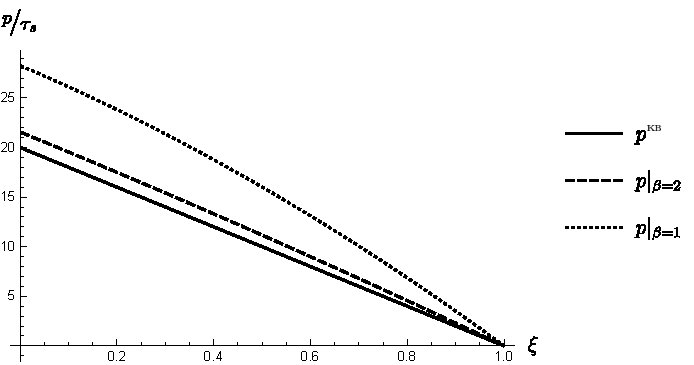
\includegraphics[scale=1.3]{./ch2/pressure_sub1}
    }
    \caption{Эпюры давления для случая цилиндрического слоя при радиусах цилиндров порядка толщины слоя}
    \label{fig:ch2/sec3/pressure}
\end{figure}

Пользуясь тем, что в случае $c=1$ имеет место равенство $\mathcal{V}_0 / \pi~=~\left(2a + 1\right) h^{3} / \alpha$, где $\mathcal{V}_0$ -- объем слоя, а высота слоя $h$ представима в виде $h=V \left(t_*-t\right)$, можно установить зависимость между временем и стадией прессования:
\begin{equation}
  t_* - t \sim \frac{\text{Eu}^{\nicefrac{-1}{3\beta}}}{V}\sqrt[3]{\frac{\mathcal{V}_0}{\pi(2a+1)}}
\end{equation}

\section{Построение решения при радиусах цилиндров порядка длины образующей}\label{sec:ch2/sec4}

При данном соотношении дробь $\frac{\alpha}{\alpha\rho+a \alpha^c}$ с учетом малости параметра примет вид $\frac{\alpha}{\alpha\rho+a} = \frac{\alpha}{a}\left(1-\frac{\alpha\rho}{a}+\cdots\right) = \frac{\alpha}{a} + O\left(\alpha^2\right)$.

\subsection{Переход от квазистатического к динамическому режиму деформирования}\label{subsec:ch2/sec4/sub1}

Рассмотрим случай $\beta=2$, который соответствует моменту перехода от квазистатического к динамическому режиму деформирования.

Положим $\text{Eu}^{-1} = C_2 \alpha^2$ и последовательно приравняем коэффициенты правых и левых частей уравнений системы \cref{eqs:ch2/sec1/substituted} при $a^{-1}$ и $\alpha^0$:
\begingroup
\allowdisplaybreaks
\begin{subequations}
  \label{eqs:ch2/sec4/sub1/main}
  \begin{gather}
    \label{eqs:ch2/sec4/sub1/-1/motion:2}
    -\uindex{p}{-1}_{,\rho} = 0
    \\
    \label{eqs:ch2/sec4/sub1/-1/coax:2}
    \uindex{s}{0}_{rr} \; \uindex{v}{-1}_{z,\rho} = 0
    \\
    \label{eqs:ch2/sec4/sub1/0/motion:1}
    -\uindex{p}{0}_{,\rho}+\uindex{s}{0}_{rr,\rho} = 0
    \\
    \label{eqs:ch2/sec4/sub1/0/motion:2}
    -\uindex{p}{-1}_{,\xi} + \uindex{s}{0}_{rz,\rho} = 0
    \\
    \label{eqs:ch2/sec4/sub1/0/plasticity}
    \left(\uindex{s}{0}_{rr}\right)^2 + \left(\uindex{s}{0}_{\theta\theta}\right)^2 + \uindex{s}{0}_{rr}\; \uindex{s}{0}_{\theta\theta} + \left(\uindex{s}{0}_{rz}\right)^2 = 1
    \\
    \label{eqs:ch2/sec4/sub1/0/coax:1}
    0 = \uindex{s}{0}_{\theta\theta} \uindex{v}{0}_{r,\rho}
    \\
    \label{eqs:ch2/sec4/sub1/0/coax:2}
    \uindex{s}{0}_{rr} \; \uindex{v}{0}_{z,\rho} = 2 \uindex{s}{0}_{rz} \; \uindex{v}{0}_{r,\rho}
    \\
    \label{eqs:ch2/sec4/sub1/0/uncompress}
    \uindex{v}{0}_{r,\rho} + \uindex{v}{-1}_{z,\xi} = 0
  \end{gather}
\end{subequations}
\endgroup
Граничные условия \cref{eq:ch2/sec1/boundary/kinematic, eq:ch2/sec1/boundary/force} при этом примут вид
\begin{equation}
  \label{eq:ch2/sec4/sub1/boundary/0}
  \uindex{v}{0}_{r}\lvert_{\rho=0} = 1,\quad \uindex{v}{0}_{r}\lvert_{\rho=1} = 0, \quad \lvert \uindex{s}{0}_{rz}\lvert_{\rho=0} = \lvert \uindex{s}{0}_{rz}\lvert_{\rho=1} = \mu
\end{equation}
Из уравнений \cref{eqs:ch2/sec4/sub1/-1/motion:2, eqs:ch2/sec4/sub1/-1/coax:2} вытекает
\begin{equation*}
  \uindex{p}{-1} = \uindex{f}{-1}_{p}(\xi, \tau), \quad \uindex{v}{-1}_{z} = \uindex{f}{-1}_{v_{z}}(\xi, \tau).
\end{equation*}
Подставив выражение $\uindex{v}{-1}_{z}$ в уравнение \cref{eqs:ch2/sec4/sub1/0/uncompress} и решив дифференциальное уравнение, получим выражение для $\uindex{v}{0}_{r}$:
\begin{equation*}
  \uindex{v}{0}_{r} = \uindex{f}{0}_{v_{r}}(\xi, \tau) -\rho \uindex{f}{-1}_{v_{z},\xi}
\end{equation*}
Подстановка данного равенства в кинематические граничные условия \cref{eq:ch2/sec4/sub1/boundary/0} позволяет определить неизвестные функции интегрирования:
\begin{gather*}
  \uindex{f}{0}_{v_{r}} = 1
  \\
  \uindex{f}{-1}_{v_{z}} = \xi + \uindex{g}{-1}_{v_{z}}(\tau)
\end{gather*}
В силу рассуждений приведенных в предыдущем пункте можно положить $\uindex{g}{-1}_{v_{z}}(\tau) = 0$. Окончательно получаем
\begin{gather}
  \label{sol:ch2/sec4/sub1/vz/-1}
  \uindex{v}{-1}_{z} = \uindex{f}{-1}_{v_{z}} = \xi
  \\
  \label{sol:ch2/sec4/sub1/vr/0}
  \uindex{v}{0}_{r} =  1 - \rho
\end{gather}
Решая \cref{eqs:ch2/sec4/sub1/0/motion:2} относительно $\uindex{s}{0}_{rz}$ и используя силовые граничные условия \cref{eq:ch2/sec4/sub1/boundary/0} придем к
\begin{gather*}
  \uindex{s}{0}_{rz} = \uindex{f}{0}_{s_{rz}}(\xi, \tau) + \rho \uindex{f}{-1}_{p,\xi}
  \\
  \uindex{f}{0}_{s_{rz}} = \mu\hat{s}, \quad \hat{s} = \pm 1
  \\
  \mu\hat{s} +\uindex{f}{-1}_{p,\xi} = -\mu \hat{s},
  \\
  \uindex{p}{-1}=\uindex{f}{-1}_{p} =\uindex{g}{-1}_{p}(\tau) -2\mu\hat{s}\xi
\end{gather*}

В силу тех же рассуждений, что приводились в \ref{subsec:ch2/sec2/sub1} следует положить $\hat{s}~=~\sign\xi$. Тогда найденные функции можно записать в следующем виде:
\begin{gather}
  \label{sol:ch2/sec4/sub1/srz/0}
  \uindex{s}{0}_{rz} = -\mu \left(2\rho - 1\right) \sign \xi
  \\
  \label{sol:ch2/sec4/sub1/p/-1}
  \uindex{p}{-1} = \uindex{g}{-1}_{p}(\tau) -2\mu\lvert\xi\rvert = 2\mu\left(1-\lvert\xi\rvert\right) + \uindex{p}{-1}_{0}(\tau)
\end{gather}
С учетом найденных функций \cref{eqs:ch2/sec4/sub1/0/coax:1, eqs:ch2/sec4/sub1/0/plasticity} представляют собой алгебраическую систему уравнений относительно $\uindex{s}{0}_{rr}$ и $\uindex{s}{0}_{\theta\theta}$, решив которую, найдем
\begin{gather}
  \label{sol:ch2/sec4/sub1/srr/0}
  \uindex{s}{0}_{rr} = -\sqrt{1-\left(\uindex{s}{0}_{rz}\right)^2} = -\sqrt{1-\mu^2\left(2\rho-1\right)^2}
  \\
  \label{sol:ch2/sec4/sub1/stt/0}
  \uindex{s}{0}_{\theta\theta} = 0
\end{gather}
Подставив все найденные функции в \cref{eqs:ch2/sec4/sub1/0/motion:1, eqs:ch2/sec4/sub1/0/coax:2} и решив дифференциальные уравнения найдем:
\begin{gather}
  \label{sol:ch2/sec4/sub1/vz/0}
  \uindex{v}{0}_{z} = \frac{\sign\xi}{\mu}\sqrt{1-\mu^2\left(2\rho-1\right)^2} + \uindex{f}{0}_{v_{z}}(\xi,\tau),
  \\
  \label{sol:ch2/sec4/sub1/p/0}
  \uindex{p}{0} = \uindex{s}{0}_{rr} +\uindex{f}{0}_{p}(\xi,\tau)
\end{gather}
Для нахождение неизвестных функций $\uindex{f}{0}_{p}$ и $\uindex{f}{0}_{v_{z}}$ выпишем следующее по $\alpha$ приближение уравнений \cref{eqs:ch2/sec1/substituted/motion:2, eqs:ch2/sec1/substituted/uncompress}, а также граничные условия \cref{eq:ch2/sec1/boundary/kinematic, eq:ch2/sec1/boundary/force}:
\begin{subequations}
  \begin{gather}
    \label{eqs:ch2/sec4/sub1/1/motion:1}
    -\uindex{p}{0}_{,\xi} + \uindex{s}{1}_{rz,\rho} + \uindex{s}{0}_{rz} / a = C_2 \left(3\xi\right)
    \\
    \label{eqs:ch2/sec4/sub1/1/uncompress}
    \uindex{v}{1}_{r,\rho} + \uindex{v}{0}_{r} / a + \uindex{v}{0}_{z,\xi} = 0
    \\
    \label{eq:ch2/sec4/sub1/boundary/1}
    \uindex{v}{1}_{r}\lvert_{\rho=0} = \uindex{v}{1}_{r}\lvert_{\rho=1} = 0, \quad \lvert \uindex{s}{1}_{rz}\lvert_{\rho=0} = \lvert \uindex{s}{1}_{rz}\lvert_{\rho=1} = 0
  \end{gather}
\end{subequations}
Из уравнения \cref{eqs:ch2/sec4/sub1/1/uncompress} с учетом граничных условий \cref{eq:ch2/sec4/sub1/boundary/1} найдем
\begin{gather*}
  \uindex{v}{1}_{r} = \uindex{f}{1}_{v_{r}}(\xi, \tau) - \frac{\rho}{a}\left(1-\frac{\rho}{2}\right) -\rho \uindex{f}{0}_{v_{z},\xi}
  \\
  \uindex{f}{1}_{v_{r}} = 0, \quad \uindex{f}{0}_{v_{z}}= -\xi / 2a + \uindex{g}{0}_{v_{z}}(\tau)
\end{gather*}
Применяя рассуждения, использованные при выводе \cref{sol:ch2/sec4/sub1/vz/-1}, получим $\uindex{g}{0}_{v_{z}} = 0$. Оставшееся уравнение \cref{eqs:ch2/sec4/sub1/1/motion:1} даст выражение для $\uindex{s}{1}_{rz}$:
\begin{equation*}
  \uindex{s}{1}_{rz} = \uindex{f}{1}_{s_{rz}}(\xi, \tau) + \rho \uindex{f}{0}_{p,\xi} + 3C_2 \xi \rho - \frac{\mu}{a}\rho(1-\rho)\sign\xi
\end{equation*}
С учетом силовых граничных условий \cref{eq:ch2/sec4/sub1/boundary/1} получим
\begin{gather*}
  \uindex{f}{1}_{s_{rz}} = 0, \quad
  3C_2 \xi + \uindex{f}{0}_{p,\xi} = 0
  \\
  \uindex{f}{0}_{p} = \uindex{g}{0}_{p}(\tau) - \frac{3 C_2}{2} \xi^2 = \frac{3 C_2}{2}\left(1-\xi^2\right) + \uindex{p}{0}_{0}(\tau)
\end{gather*}
\subsection{Развитый процесс динамического деформирования}\label{subsec:ch2/sec4/sub2}

Рассмотрим случай $\beta=1$, который соответствует моменту с сильным влиянием динамики в процессе сдавливания слоя.


Положим $\text{Eu}^{-1} = C_1 \alpha$ и последовательно приравняем коэффициенты правых и левых частей уравнений системы \cref{eqs:ch2/sec1/substituted} при $a^{-1}$ и $\alpha^0$:
\begin{subequations}
  \label{eqs:ch2/sec4/sub2/main}
  \begin{gather}
    \label{eqs:ch2/sec4/sub2/-1/motion:2}
    -\uindex{p}{-1}_{,\rho} = 0
    \\
    \label{eqs:ch2/sec4/sub2/-1/coax:2}
    \uindex{s}{0}_{rr} \; \uindex{v}{-1}_{z,\rho} = 0
    \\
    \label{eqs:ch2/sec4/sub2/0/motion:1}
    -\uindex{p}{0}_{,\rho}+\uindex{s}{0}_{rr,\rho} = 0
    \\
    \label{eqs:ch2/sec4/sub2/0/motion:2}
    -\uindex{p}{-1}_{,\xi} + \uindex{s}{0}_{rz,\rho} = C_1 \left((\rho-1) \ \uindex{v}{-1}_{z,\rho} + (1+\tau) \ \uindex{v}{-1}_{z,\tau} + 2 \ \uindex{v}{-1}_{z} + \uindex{v}{0}_{r} \ \uindex{v}{-1}_{z,\rho} + \uindex{v}{-1}_{z} \ \uindex{v}{-1}_{z,\xi} \right)
    \\
    \label{eqs:ch2/sec4/sub2/0/plasticity}
    \left(\uindex{s}{0}_{rr}\right)^2 + \left(\uindex{s}{0}_{\theta\theta}\right)^2 + \uindex{s}{0}_{rr}\; \uindex{s}{0}_{\theta\theta} + \left(\uindex{s}{0}_{rz}\right)^2 = 1
    \\
    \label{eqs:ch2/sec4/sub2/0/coax:1}
    0 = \uindex{s}{0}_{\theta\theta} \uindex{v}{0}_{r,\rho}
    \\
    \label{eqs:ch2/sec4/sub2/0/coax:2}
    \uindex{s}{0}_{rr} \; \uindex{v}{0}_{z,\rho} = 2 \ \uindex{s}{0}_{rz} \; \uindex{v}{0}_{r,\rho}
    \\
    \label{eqs:ch2/sec4/sub2/0/uncompress}
    \uindex{v}{0}_{r,\rho} + \uindex{v}{-1}_{z,\xi} = 0
  \end{gather}
\end{subequations}
Граничные условия \cref{eq:ch2/sec1/boundary/kinematic, eq:ch2/sec1/boundary/force} при этом примут вид
\begin{equation}
  \label{eq:ch2/sec4/sub2/boundary/0}
  \uindex{v}{0}_{r}\lvert_{\rho=0} = 1,\quad \uindex{v}{0}_{r}\lvert_{\rho=1} = 0, \quad \lvert \uindex{s}{0}_{rz}\lvert_{\rho=0} = \lvert \uindex{s}{0}_{rz}\lvert_{\rho=1} = \mu
\end{equation}
Из уравнений \cref{eqs:ch2/sec4/sub2/-1/motion:2, eqs:ch2/sec4/sub2/-1/coax:2} вытекает
\begin{equation*}
  \uindex{p}{-1} = \uindex{f}{-1}_{p}(\xi, \tau), \quad \uindex{v}{-1}_{z} = \uindex{f}{-1}_{v_{z}}(\xi, \tau).
\end{equation*}
Подставив выражение $\uindex{v}{-1}_{z}$ в уравнение \cref{eqs:ch2/sec4/sub2/0/uncompress} и решив дифференциальное уравнение, получим выражение для $\uindex{v}{0}_{r}$:
\begin{equation*}
  \uindex{v}{0}_{r} = \uindex{f}{0}_{v_{r}}(\xi, \tau) -\rho \uindex{f}{-1}_{v_{z},\xi}
\end{equation*}
Подстановка данного равенства в кинематические граничные условия \cref{eq:ch2/sec4/sub2/boundary/0} позволяет определить неизвестные функции интегрирования:
\begin{gather*}
  \uindex{f}{0}_{v_{r}} = 1
  \\
  \uindex{f}{-1}_{v_{z}} = \xi + \uindex{g}{-1}_{v_{z}}(\tau)
\end{gather*}
В силу рассуждений приведенных в предыдущем пункте можно положить $\uindex{g}{-1}_{v_{z}}(\tau) = 0$. Окончательно получаем
\begin{gather}
  \label{sol:ch2/sec4/sub2/vz/-1}
  \uindex{v}{-1}_{z} = \uindex{f}{-1}_{v_{z}} = \xi
  \\
  \label{sol:ch2/sec4/sub2/vr/0}
  \uindex{v}{0}_{r} =  1 - \rho
\end{gather}
С учетом \cref{sol:ch2/sec4/sub2/vz/-1} уравнение \cref{eqs:ch2/sec4/sub2/0/motion:2} примет вид
\begin{equation*}
  -\uindex{p}{-1}_{,\xi} + \uindex{s}{0}_{rz,\rho} = C_1 \left(3 \xi \right)
\end{equation*}
Решая его относительно $\uindex{s}{0}_{rz}$ и используя силовые граничные условия \cref{eq:ch2/sec4/sub2/boundary/0} придем к
\begin{gather*}
  \uindex{s}{0}_{rz} = \uindex{f}{0}_{s_{rz}}(\xi, \tau) + \rho \uindex{f}{-1}_{p,\xi} + 3 C_1 \rho \xi
  \\
  \uindex{f}{0}_{s_{rz}} = \mu\hat{s}, \quad \hat{s} = \pm 1
  \\
  \mu\hat{s} +\uindex{f}{-1}_{p,\xi} + 3 C_1 \rho \xi = -\mu \hat{s},
  \\
  \uindex{p}{-1}=\uindex{f}{-1}_{p} =\uindex{g}{-1}_{p}(\tau) -2\mu\hat{s}\xi - \frac{3 C_1}{2}\xi^2
\end{gather*}

В силу тех же рассуждений, что приводились в \ref{subsec:ch2/sec2/sub1} следует положить $\hat{s}~=~\sign\xi$. Тогда найденные функции можно записать в следующем виде:
\begin{gather}
  \label{sol:ch2/sec4/sub2/srz/0}
  \uindex{s}{0}_{rz} = -\mu \left(2\rho - 1\right) \sign \xi
  \\
  \label{sol:ch2/sec4/sub2/p/-1}
  \uindex{p}{-1} = \uindex{g}{-1}_{p}(\tau) -2\mu\lvert\xi\rvert - \frac{3 C_1}{2}\xi^2 = 2\mu\left(1-\lvert\xi\rvert\right) + \frac{3 C_1}{2}\left(1-\xi^2\right) + \uindex{p}{-1}_{0}(\tau)
\end{gather}
С учетом найденных функций \cref{eqs:ch2/sec4/sub2/0/coax:1, eqs:ch2/sec4/sub2/0/plasticity} представляют собой алгебраическую систему уравнений относительно $\uindex{s}{0}_{rr}$ и $\uindex{s}{0}_{\theta\theta}$, решив которую, найдем
\begin{gather}
  \label{sol:ch2/sec4/sub2/srr/0}
  \uindex{s}{0}_{rr} = -\sqrt{1-\left(\uindex{s}{0}_{rz}\right)^2} = -\sqrt{1-\mu^2\left(2\rho-1\right)^2}
  \\
  \label{sol:ch2/sec4/sub2/stt/0}
  \uindex{s}{0}_{\theta\theta} = 0
\end{gather}
Подставив все найденные функции в \cref{eqs:ch2/sec4/sub2/0/motion:1, eqs:ch2/sec4/sub2/0/coax:2} и решив дифференциальные уравнения найдем:
\begin{gather}
  \label{sol:ch2/sec4/sub2/vz/0}
  \uindex{v}{0}_{z} = \frac{\sign\xi}{\mu}\sqrt{1-\mu^2\left(2\rho-1\right)^2} + \uindex{f}{0}_{v_{z}}(\xi,\tau),
  \\
  \label{sol:ch2/sec4/sub2/p/0}
  \uindex{p}{0} = \uindex{s}{0}_{rr} +\uindex{f}{0}_{p}(\xi,\tau)
\end{gather}
Для нахождение неизвестных функций $\uindex{f}{0}_{p}$ и $\uindex{f}{0}_{v_{z}}$ выпишем следующее по $\alpha$ приближение уравнений \cref{eqs:ch2/sec1/substituted/motion:2, eqs:ch2/sec1/substituted/uncompress}, а также граничные условия \cref{eq:ch2/sec1/boundary/kinematic, eq:ch2/sec1/boundary/force}:
\begin{subequations}
  \begin{gather}
    \label{eqs:ch2/sec4/sub2/1/motion:1}
    -\uindex{p}{0}_{,\xi} + \uindex{s}{1}_{rz,\rho} + \uindex{s}{0}_{rz} / a = C_1 \left(-\left(1-\frac{1}{2a}\right)\xi + (1+\tau) \ \uindex{v}{0}_{z,\tau} + \uindex{v}{0}_{z} + \xi \ \uindex{v}{0}_{z,\xi}\vphantom{\frac{1}{2a}}\right)
    \\
    \label{eqs:ch2/sec4/sub2/1/uncompress}
    \uindex{v}{1}_{r,\rho} + \uindex{v}{0}_{r} / a + \uindex{v}{0}_{z,\xi} = 0
    \\
    \label{eq:ch2/sec4/sub2/boundary/1}
    \uindex{v}{1}_{r}\lvert_{\rho=0} = \uindex{v}{1}_{r}\lvert_{\rho=1} = 0, \quad \lvert \uindex{s}{1}_{rz}\lvert_{\rho=0} = \lvert \uindex{s}{1}_{rz}\lvert_{\rho=1} = 0
  \end{gather}
\end{subequations}
Из уравнения \cref{eqs:ch2/sec4/sub2/1/uncompress} с учетом граничных условий \cref{eq:ch2/sec4/sub2/boundary/1} найдем
\begin{gather*}
  \uindex{v}{1}_{r} = \uindex{f}{1}_{v_{r}}(\xi, \tau) - \frac{\rho}{a}\left(1-\frac{\rho}{2}\right) -\rho \uindex{f}{0}_{v_{z},\xi}
  \\
  \uindex{f}{1}_{v_{r}} = 0, \quad \uindex{f}{0}_{v_{z}}= -\xi / 2a + \uindex{g}{0}_{v_{z}}(\tau)
\end{gather*}
Применяя рассуждения, использованные при выводе \cref{sol:ch2/sec4/sub2/vz/-1}, получим $\uindex{g}{0}_{v_{z}} = 0$. Оставшееся уравнение \cref{eqs:ch2/sec4/sub2/1/motion:1} после подстановки $\uindex{v}{0}_{z}$ даст выражение для $\uindex{s}{1}_{rz}$:
\begin{equation*}
  \begin{multlined}
    \uindex{s}{1}_{rz} = \uindex{f}{1}_{s_{rz}}(\xi, \tau) + \rho \uindex{f}{0}_{p,\xi} + \frac{(3+2a)C_1 \xi \rho}{2a} - \frac{\mu}{a}\rho(1-\rho)\sign\xi \unl{-} \frac{C_1}{4\mu}\left(\sqrt{1-\mu^2\left(2\rho-1\right)^2} \left(1-2\rho\right)+\frac{\arcsin{\left(\mu\left(1-2\rho\right)\right)}}{\mu}\right)\sign\xi
  \end{multlined}
\end{equation*}
С учетом силовых граничных условий \cref{eq:ch2/sec4/sub2/boundary/1} получим
\begin{gather*}
  \uindex{f}{1}_{s_{rz}} - \frac{C_1}{4\mu}\left(\sqrt{1-\mu^2} + \frac{\arcsin{\left(\mu\right)}}{\mu}\right)\sign{\xi}= 0
  \\
  \frac{C_1}{2\mu}\left(\sqrt{1-\mu^2} + \frac{\arcsin{\left(\mu\right)}}{\mu}\right)\sign{\xi}-\frac{(3+2a)C_1 \xi}{2a} + \uindex{f}{0}_{p,\xi} = 0
  \\
  \uindex{f}{0}_{p} = \uindex{g}{0}_{p}(\tau) + \frac{(3+2a)C_1 \xi^2}{2a} - \frac{C_1 \lvert\xi\rvert}{2\mu^2}\left(\mu\sqrt{1-\mu^2}+\arcsin{\left(\mu\right)}\right)
\end{gather*}

\section{Анализ решения для случая, когда радиусы цилиндров порядка длины образующей}\label{sec:ch2/sec5}

Полученные решения \cref{sol:ch2/sec4/sub1/p/-1,sol:ch2/sec4/sub1/srz/0,sol:ch2/sec4/sub1/vz/-1,sol:ch2/sec4/sub1/vz/0,sol:ch2/sec4/sub1/srr/0, sol:ch2/sec4/sub1/stt/0,sol:ch2/sec4/sub1/vr/0,sol:ch2/sec4/sub1/p/0,sol:ch2/sec4/sub1/vz/0} и \cref{sol:ch2/sec4/sub2/p/-1,sol:ch2/sec4/sub2/srz/0,sol:ch2/sec4/sub2/vz/-1,sol:ch2/sec4/sub2/vz/0,sol:ch2/sec4/sub2/srr/0, sol:ch2/sec4/sub2/stt/0,sol:ch2/sec4/sub2/vr/0,sol:ch2/sec4/sub2/p/0,sol:ch2/sec4/sub2/vz/0} являются приближенными и с точностью $O(\alpha)$ совпадают, за исключением функции давления, с квазистатическим решением \autocite{Georgievsky:2010}:
\todo{Переписать решение}
\begin{subequations}
  \begin{gather}
    \label{sol:ch2/sec5/p/qs}
    p  = p_0 + \frac{2\mu}{\alpha}\left(1-\lvert\xi\rvert\right)\tau_{s} + s_{rr} + O(\alpha)
    \\
    s_{rr} = -\sqrt{\tau_{s}^2-s_{rz}^2} + O(\alpha)
    \\
    s_{\theta\theta} = O(\alpha)
    \\
    s_{rz} = -\mu \left(2\rho - 1\right) \sign \xi \tau_{s}  + O(\alpha)
    \\
    v_{r} = V\left(1-\rho\right) + O(\alpha)
    \\
    v_{z} / V = \frac{\xi}{\alpha} + \frac{\sign\xi}{\mu}\sqrt{1-\mu^2\left(2\rho-1\right)^2} - \frac{\xi}{2a} +  O(\alpha)
  \end{gather}
\end{subequations}
где $p_0$ имеет смысл гидростатического давления.

Наличие сигнатуры $\sign\xi$ в функции $s_{rz}$ говорит о разрыве решения вблизи сечения $\xi=0$. Следовательно, разложения \cref{eqs:ch2/series} несправедливы вблизи среднего по простиранию сечения слоя. Кроме того, данное решение неприменимо в зоне краевого эффекта, то есть вблизи сечений $\xi=\pm 1$, где необходимо ставить точные граничные условия. Данные ограничения аналогичны трактуемым в анализе решения классической задачи Прандтля.

Обозначим правую часть уравнения \cref{sol:ch2/sec5/p/qs} как $p^\text{кв}$. Для случаев $\beta=2$ и $\beta=1$ имеем соответственно:
\begin{gather}
  \left(p\lvert_{\beta=2}\right) = p^\text{кв} + \frac{3 C_2}{2}\left(1-\xi^2\right) \tau_{s}
  \\
  \begin{multlined}
    \left(p\lvert_{\beta=1}\right) / \tau_{s} = p^\text{кв} / \tau_{s} + \frac{3C_1}{2\alpha} \left(1-\xi^2\right) + \frac{(3+2a)C_1 \xi^2}{2a} \unl{-} \frac{C_1 \lvert\xi\rvert}{2\mu^2}\left(\mu\sqrt{1-\mu^2}+\arcsin{\left(\mu\right)}\right)
  \end{multlined}
\end{gather}
При сравнении выражений видно, что в случае динамического сдавливания возникает квадратично зависящее от радиуса слагаемое, причем, чем динамичнее происходит процесс, тем более значима становится данная величина. Наличие такой зависимости качественно меняет эпюру давления в слое и увеличивает суммарную силу, действующую со стороны слоя на плиты.

На графике ниже приведены эпюры давления для различных стадий процесса при следующих параметрах: $\alpha=0.1$, $C_1=1$, $C_2=2$, $\mu=1$, $a=1$.
\begin{figure}[ht]
  \centerfloat{
    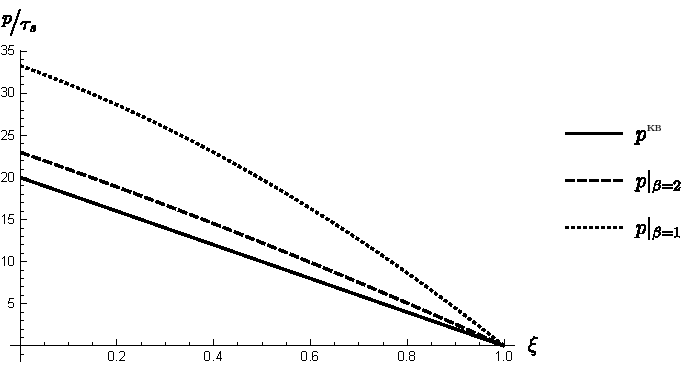
\includegraphics[scale=1.3]{./ch2/pressure_sub2}
    }
    \caption{Эпюры давления для случая цилиндрического слоя при радиусах цилиндров порядка длины образующей}
    \label{fig:ch2/sec5/pressure}
\end{figure}

Пользуясь тем, что в случае $c=0$ имеет место равенство $\mathcal{V}_0 / \pi~=~\left(2a + \alpha\right) h^{3} / \alpha^{2}$, где $\mathcal{V}_0$ -- объем слоя, а высота слоя $h$ представима в виде $h=V \left(t_*-t\right)$, можно установить зависимость между временем и стадией прессования:
\begin{equation}
  t_* - t \sim \frac{\text{Eu}^{\nicefrac{-2}{3\beta}}}{V}\sqrt[3]{\frac{\mathcal{V}_0}{\pi\left(2a+\text{Eu}^{\nicefrac{-1}{\beta}}\right)}}
\end{equation}

\section{Построение решения при радиусах цилиндров ``промежуточного'' порядка малости}\label{sec:ch2/sec6}

При данном соотношении дробь $\frac{\alpha}{\alpha\rho+a \alpha^c}$ с учетом малости параметра примет вид $\frac{\alpha}{\alpha\rho+a \alpha^c} = \frac{\alpha^{1-c}}{a}\left(1-\frac{\alpha^{1-c}\rho}{a}+\cdots\right) = \frac{\alpha^{1-c}}{a} + O\left(\alpha^{2\left(1-c\right)}\right)$.
Наличие дробной степени параметра $\alpha$ свидетельствует о непременимости целочисленных разложений \cref{eqs:ch2/series}. В связи с этим первые члены асмиптотических разложений должны быть следующие:
\begin{subequations}
  \label{eqs:ch2/sec6/series}
  \begin{gather}
    v_{r}\left(r, z, t\right) = V \left(\uindex{v}{0}_{r} + \alpha^{1-c} \;\ \uindex{v}{1-c}_{r} + \cdots\right)
    \\
    v_{z}\left(r, z, t\right) = V \left(\alpha^{-1} \; \uindex{v}{-1}_{z} + \alpha^{-c} \;\ \uindex{v}{-c}_{z} + \uindex{v}{0}_{z} + \alpha^{1-c} \;\ \uindex{v}{1-c}_{z} + \cdots\right)
    \\
    s_{ij}\left(r, z, t\right) = \tau_{s} \left(\uindex{s}{0}_{ij} + \alpha^{1-c} \;\ \uindex{s}{1-c}_{ij} + \cdots\right), \quad (ij)\in\{rr, rz, \theta\theta\}
    \\
    p\left(r, z, t \right) = \tau_{s} \left(\alpha^{-1} \; \uindex{p}{-1} + \alpha^{-c} \; \uindex{p}{-c} + \uindex{p}{0} + \alpha^{1-c} \;\ \uindex{p}{1-c} + \cdots\right)
  \end{gather}
\end{subequations}
В общем случае, однозначно определить порядок следующего за $\alpha^{1-c}$ члена разложение не представляется возможным: он может быть равен $\alpha^{2(1-c)}$ или $\alpha$. Вообще говоря, для $c\in(0,1)$ существует счетное количество возможных вариантов разложений, поэтому, не останавливаясь на детальном анализе частных случаев, ограничимся отысканием решений для любого $c$ из заданного интервала для коэффициентов $\alpha^{-1}$, $\alpha^{-c}$, $\alpha^0$ и $\alpha^{1-c}$. 
\subsection{Переход от квазистатического к динамическому режиму деформирования}\label{subsec:ch2/sec6/sub1}

Рассмотрим случай $\beta=2$, который соответствует моменту перехода от квазистатического к динамическому режиму деформирования.

Положим $\text{Eu}^{-1} = C_2 \alpha^2$ и подставим разложения \cref{eqs:ch2/sec6/series} в \cref{eqs:ch2/sec1/general,eq:ch2/sec1/boundary/kinematic, eq:ch2/sec1/boundary/force}. Последовательное приравнивание коэффициентов правых и левых частей уравнений полученной системы при $a^{-1}$ и $\alpha^0$ даст
\begin{subequations}
  \label{eqs:ch2/sec6/sub1/main/int}
  \begin{gather}
    \label{eqs:ch2/sec6/sub1/-1/motion:2}
    -\uindex{p}{-1}_{,\rho} = 0
    \\
    \label{eqs:ch2/sec6/sub1/-1/coax:2}
    \uindex{s}{0}_{rr} \; \uindex{v}{-1}_{z,\rho} = 0
    \\
    \label{eqs:ch2/sec6/sub1/0/motion:1}
    -\uindex{p}{0}_{,\rho}+\uindex{s}{0}_{rr,\rho} = 0
    \\
    \label{eqs:ch2/sec6/sub1/0/motion:2}
    -\uindex{p}{-1}_{,\xi} + \uindex{s}{0}_{rz,\rho} = 0
    \\
    \label{eqs:ch2/sec6/sub1/0/plasticity}
    \left(\uindex{s}{0}_{rr}\right)^2 + \left(\uindex{s}{0}_{\theta\theta}\right)^2 + \uindex{s}{0}_{rr}\; \uindex{s}{0}_{\theta\theta} + \left(\uindex{s}{0}_{rz}\right)^2 = 1
    \\
    \label{eqs:ch2/sec6/sub1/0/coax:1}
    0 = \uindex{s}{0}_{\theta\theta} \uindex{v}{0}_{r,\rho}
    \\
    \label{eqs:ch2/sec6/sub1/0/coax:2}
    \uindex{s}{0}_{rr} \; \uindex{v}{0}_{z,\rho} = 2 \uindex{s}{0}_{rz} \; \uindex{v}{0}_{r,\rho}
    \\
    \label{eqs:ch2/sec6/sub1/0/uncompress}
    \uindex{v}{0}_{r,\rho} + \uindex{v}{-1}_{z,\xi} = 0
    \\
    \label{eq:ch2/sec6/sub1/boundary/0}
    \uindex{v}{0}_{r}\lvert_{\rho=0} = 1,\quad \uindex{v}{0}_{r}\lvert_{\rho=1} = 0, \quad \lvert \uindex{s}{0}_{rz}\lvert_{\rho=0} = \lvert \uindex{s}{0}_{rz}\lvert_{\rho=1} = \mu
  \end{gather}
\end{subequations}
Процесс решения данной системы полностью приведен в секции \cref{subsec:ch2/sec4/sub1}, поэтому не повторяя выкладок приведем лишь финальный результат:
\begingroup
\allowdisplaybreaks
\begin{subequations}
  \label{sol:ch2/sec6/sub1/main/int}
  \begin{gather}
    \label{sol:ch2/sec6/sub1/vz/-1}
    \uindex{v}{-1}_{z} = \xi
    \\
    \label{sol:ch2/sec6/sub1/vr/0}
    \uindex{v}{0}_{r} =  1 - \rho
    \\
    \label{sol:ch2/sec6/sub1/srz/0}
    \uindex{s}{0}_{rz} = -\mu \left(2\rho - 1\right) \sign \xi
    \\
    \label{sol:ch2/sec6/sub1/p/-1}
    \uindex{p}{-1} = 2\mu\left(1-\lvert\xi\rvert\right) + \uindex{p}{-1}_{0}(\tau)
    \\
    \label{sol:ch2/sec6/sub1/srr/0}
    \uindex{s}{0}_{rr} = -\sqrt{1-\left(\uindex{s}{0}_{rz}\right)^2} = -\sqrt{1-\mu^2\left(2\rho-1\right)^2}
    \\
    \label{sol:ch2/sec6/sub1/stt/0}
    \uindex{s}{0}_{\theta\theta} = 0
    \\
    \label{sol:ch2/sec6/sub1/vz/0}
    \uindex{v}{0}_{z} = \frac{\sign\xi}{\mu}\sqrt{1-\mu^2\left(2\rho-1\right)^2} + \uindex{f}{0}_{v_{z}}(\xi,\tau),
    \\
    \label{sol:ch2/sec6/sub1/p/0}
    \uindex{p}{0} = \uindex{s}{0}_{rr} +\uindex{f}{0}_{p}(\xi,\tau)
  \end{gather}
\end{subequations}
\endgroup
Функции $\uindex{f}{0}_{v_{z}}(\xi,\tau)$ и $\uindex{f}{0}_{p}(\xi,\tau)$ будут отличаться от ранее найденных и в данном случае останутся неизвестными.

Перейдем к рассмотрению системы при $a^{-c}$ и $\alpha^{1-c}$:
\begin{subequations}
  \label{eqs:ch2/sec6/sub1/main/float}
  \begin{gather}
    \label{eqs:ch2/sec6/sub1/-c/motion:2}
    -\uindex{p}{-c}_{,\rho} = 0
    \\
    \label{eqs:ch2/sec6/sub1/-c/coax:2}
    \uindex{s}{0}_{rr} \; \uindex{v}{-c}_{z,\rho} = 0
    \\
    \label{eqs:ch2/sec6/sub1/1-c/motion:1}
    -\uindex{p}{1-c}_{,\rho}+\uindex{s}{1-c}_{rr,\rho} +\left(\uindex{s}{0}_{rr}-\uindex{s}{0}_{\theta\theta}\right) / a = 0
    \\
    \label{eqs:ch2/sec6/sub1/1-c/motion:2}
    -\uindex{p}{-c}_{,\xi} + \uindex{s}{1-c}_{rz,\rho} + \uindex{s}{0}_{rz} / a = 0
    \\
    \label{eqs:ch2/sec6/sub1/1-c/plasticity}
    \uindex{s}{1-c}_{rr} \left(2 \ \uindex{s}{0}_{rr} + \uindex{s}{0}_{\theta\theta}\right) + 
      \uindex{s}{1-c}_{\theta\theta} \left(\uindex{s}{0}_{rr} + 2 \ \uindex{s}{0}_{\theta\theta}\right) + 
        \uindex{s}{1-c}_{rz} \ \uindex{s}{0}_{rz} = 0
    \\
    \label{eqs:ch2/sec6/sub1/1-c/coax:1}
    \uindex{s}{0}_{rr} \uindex{v}{0}_{r} / a = \uindex{s}{1-c}_{\theta\theta} \uindex{v}{0}_{r,\rho} + \uindex{s}{0}_{\theta\theta} \; \uindex{v}{1-c}_{r,\rho}
    \\
    \label{eqs:ch2/sec6/sub1/1-c/coax:2}
    \uindex{s}{1-c}_{rr} \; \uindex{v}{0}_{z,\rho} + \uindex{s}{1-c}_{rr} \; \uindex{v}{0}_{z,\rho} =
      2 \left(\; \uindex{s}{1-c}_{rz} \; \uindex{v}{0}_{r,\rho} + \uindex{s}{0}_{rz} \; \uindex{v}{1-c}_{r,\rho} \right)
    \\
    \label{eqs:ch2/sec6/sub1/1-c/uncompress}
    \uindex{v}{1-c}_{r,\rho} + \uindex{v}{0}_{r} / a + \uindex{v}{-c}_{z,\xi} = 0
    \\
    \label{eq:ch2/sec6/sub1/boundary/1-c}
    \uindex{v}{1-c}_{r} \ \lvert_{\rho=0} =\; \uindex{v}{1-c}_{r}\ \lvert_{\rho=1} = 0, \quad  \uindex{s}{1-c}_{rz}\lvert_{\rho=0} =\; \uindex{s}{1-c}_{rz}\lvert_{\rho=1} = 0
  \end{gather}
\end{subequations}
Из уравнений \cref{eqs:ch2/sec6/sub1/-c/motion:2, eqs:ch2/sec6/sub1/-c/coax:2} вытекает
\begin{equation*}
  \uindex{p}{-c} = \uindex{f}{-c}_{p}(\xi, \tau), \quad \uindex{v}{-c}_{z} = \uindex{f}{-c}_{v_{z}}(\xi, \tau).
\end{equation*}
Подставив выражение $\uindex{v}{-1}_{z}$ в уравнение \cref{eqs:ch2/sec6/sub1/1-c/uncompress} и решив дифференциальное уравнение, получим выражение для $\uindex{v}{1-c}_{r}$:
\begin{equation*}
  \uindex{v}{1-c}_{r} = \uindex{f}{1-c}_{v_{r}}(\xi, \tau) -\rho \uindex{f}{-c}_{v_{z},\xi} - \frac{\rho}{2a}\left(2-\rho\right)
\end{equation*}
Подстановка данного равенства в кинематические граничные условия \cref{eq:ch2/sec6/sub1/boundary/1-c} позволяет определить неизвестные функции интегрирования:
\begin{gather*}
  \uindex{f}{1-c}_{v_{r}} = 0
  \\
  \uindex{f}{-c}_{v_{z}} = -\frac{\xi}{2a} + \uindex{g}{-c}_{v_{z}}(\tau)
\end{gather*}
В силу рассуждений приведенных в предыдущей секции можно положить $\uindex{g}{-c}_{v_{z}}(\tau) = 0$. Окончательно получаем
\begin{gather}
  \label{sol:ch2/sec6/sub1/vz/-c}
  \uindex{v}{-c}_{z} = \uindex{f}{-c}_{v_{z}} = -\frac{\xi}{2a}
  \\
  \label{sol:ch2/sec6/sub1/vr/1-c}
  \uindex{v}{1-c}_{r} =  \frac{\rho}{2a}\left(1-\rho\right)
\end{gather}
Решая \cref{eqs:ch2/sec6/sub1/1-c/motion:2} относительно $\uindex{s}{1-c}_{rz}$ и используя силовые граничные условия \cref{eq:ch2/sec6/sub1/boundary/1-c} придем к
\begin{gather*}
  \uindex{s}{1-c}_{rz} = \uindex{f}{1-c}_{s_{rz}}(\xi, \tau) + \rho \uindex{f}{-c}_{p,\xi} - \frac{\mu}{a} \rho\left(1-\rho\right)\sign\xi
  \\
  \uindex{f}{1-c}_{s_{rz}} = 0
  \\
  \uindex{f}{-c}_{p,\xi} = 0
\end{gather*}
и найденные функции запишутся в следующем виде:
\begin{gather}
  \label{sol:ch2/sec6/sub1/srz/1-c}
  \uindex{s}{1-c}_{rz} = - \frac{\mu}{a} \rho\left(1-\rho\right)\sign\xi
  \\
  \label{sol:ch2/sec6/sub1/p/-c}
  \uindex{p}{-c}=\uindex{f}{-1}_{p} = \uindex{g}{-c}_{p}(\tau) = \uindex{p}{-c}_{0}(\tau)
\end{gather}
С учетом найденных функций \cref{eqs:ch2/sec6/sub1/1-c/coax:1, eqs:ch2/sec6/sub1/1-c/plasticity} представляют собой алгебраическую систему уравнений относительно $\uindex{s}{1-c}_{rr}$ и $\uindex{s}{1-c}_{\theta\theta}$, решив которую, найдем
\begin{gather}
  \label{sol:ch2/sec6/sub1/srr/1-c}
  \uindex{s}{1-c}_{rr} = -\frac{1-\rho}{2a}\frac{1-\mu^2\left(2\rho-1\right)\left(4\rho-1\right)}{\sqrt{1-\mu^2\left(2\rho-1\right)^2}}
  \\
  \label{sol:ch2/sec6/sub1/stt/1-c}
  \uindex{s}{1-c}_{\theta\theta} = \frac{1-\rho}{a}\sqrt{1-\mu^2\left(2\rho-1\right)^2}
\end{gather}
Подставив все найденные функции в \cref{eqs:ch2/sec6/sub1/1-c/motion:1, eqs:ch2/sec6/sub1/1-c/coax:2} и решив дифференциальные уравнения найдем:
\begin{gather}
  \label{sol:ch2/sec6/sub1/vz/1-c}
  \uindex{v}{1-c}_{z} = \frac{\sign\xi}{\mu}\sqrt{1-\mu^2\left(2\rho-1\right)^2} + \uindex{f}{1-c}_{v_{z}}(\xi,\tau),
  \\
  \label{sol:ch2/sec6/sub1/p/1-c}
  \begin{multlined}
    \uindex{p}{1-c} = \frac{1}{4\mu}\left(\mu\left(2\rho-1\right)\sqrt{1-\mu^2\left(2\rho-1\right)^2}+\arcsin{\left(\mu\left(2\rho-1\right)\right)}\right) \unl{+}
      \uindex{s}{1-c}_{rr} + \uindex{f}{1-c}_{p}(\xi,\tau)
  \end{multlined}
\end{gather}
Для нахождение функций $\uindex{f}{1-c}_{p}$ и $\uindex{f}{1-c}_{v_{z}}$ требуется знание следующего по $\alpha$ приближения, поэтому, аналогично $\uindex{f}{0}_{p}$ и $\uindex{f}{0}_{v_{z}}$, они останутся неизвестными.

\subsection{Развитый процесс динамического деформирования}\label{subsec:ch2/sec6/sub2}

Рассмотрим случай $\beta=1$, который соответствует моменту с сильным влиянием динамики в процессе сдавливания слоя.


Положим $\text{Eu}^{-1} = C_1 \alpha$ и подставим разложения \cref{eqs:ch2/sec6/series} в \cref{eqs:ch2/sec1/general,eq:ch2/sec1/boundary/kinematic, eq:ch2/sec1/boundary/force}. Последовательное приравнивание коэффициентов правых и левых частей уравнений полученной системы при $a^{-1}$ и $\alpha^0$ даст
\begin{subequations}
  \label{eqs:ch2/sec6/sub2/main/int}
  \begin{gather}
    \label{eqs:ch2/sec6/sub2/-1/motion:2}
    -\uindex{p}{-1}_{,\rho} = 0
    \\
    \label{eqs:ch2/sec6/sub2/-1/coax:2}
    \uindex{s}{0}_{rr} \; \uindex{v}{-1}_{z,\rho} = 0
    \\
    \label{eqs:ch2/sec6/sub2/0/motion:1}
    -\uindex{p}{0}_{,\rho}+\uindex{s}{0}_{rr,\rho} = 0
    \\
    \label{eqs:ch2/sec6/sub2/0/motion:2}
    -\uindex{p}{-1}_{,\xi} + \uindex{s}{0}_{rz,\rho} = C_1 \left((\rho-1) \ \uindex{v}{-1}_{z,\rho} + (1+\tau) \ \uindex{v}{-1}_{z,\tau} + 2 \ \uindex{v}{-1}_{z} + \uindex{v}{0}_{r} \ \uindex{v}{-1}_{z,\rho} + \uindex{v}{-1}_{z} \ \uindex{v}{-1}_{z,\xi} \right)
    \\
    \label{eqs:ch2/sec6/sub2/0/plasticity}
    \left(\uindex{s}{0}_{rr}\right)^2 + \left(\uindex{s}{0}_{\theta\theta}\right)^2 + \uindex{s}{0}_{rr}\; \uindex{s}{0}_{\theta\theta} + \left(\uindex{s}{0}_{rz}\right)^2 = 1
    \\
    \label{eqs:ch2/sec6/sub2/0/coax:1}
    0 = \uindex{s}{0}_{\theta\theta} \uindex{v}{0}_{r,\rho}
    \\
    \label{eqs:ch2/sec6/sub2/0/coax:2}
    \uindex{s}{0}_{rr} \; \uindex{v}{0}_{z,\rho} = 2 \uindex{s}{0}_{rz} \; \uindex{v}{0}_{r,\rho}
    \\
    \label{eqs:ch2/sec6/sub2/0/uncompress}
    \uindex{v}{0}_{r,\rho} + \uindex{v}{-1}_{z,\xi} = 0
    \\
    \label{eq:ch2/sec6/sub2/boundary/0}
    \uindex{v}{0}_{r}\lvert_{\rho=0} = 1,\quad \uindex{v}{0}_{r}\lvert_{\rho=1} = 0, \quad \lvert \uindex{s}{0}_{rz}\lvert_{\rho=0} = \lvert \uindex{s}{0}_{rz}\lvert_{\rho=1} = \mu
  \end{gather}
\end{subequations}
Процесс решения данной системы полностью приведен в секции \cref{subsec:ch2/sec4/sub2}, поэтому не повторяя выкладок приведем лишь финальный результат:
\begingroup
\allowdisplaybreaks
\begin{subequations}
  \label{sol:ch2/sec6/sub2/main/int}
  \begin{gather}
    \label{sol:ch2/sec6/sub2/vz/-1}
    \uindex{v}{-1}_{z} = \xi
    \\
    \label{sol:ch2/sec6/sub2/vr/0}
    \uindex{v}{0}_{r} =  1 - \rho
    \\
    \label{sol:ch2/sec6/sub2/srz/0}
    \uindex{s}{0}_{rz} = -\mu \left(2\rho - 1\right) \sign \xi
    \\
    \label{sol:ch2/sec6/sub2/p/-1}
    \uindex{p}{-1} = 2\mu\left(1-\lvert\xi\rvert\right) + \frac{3 C_1}{2}\left(1-\xi^2\right) + \uindex{p}{-1}_{0}(\tau)
    \\
    \label{sol:ch2/sec6/sub2/srr/0}
    \uindex{s}{0}_{rr} = -\sqrt{1-\left(\uindex{s}{0}_{rz}\right)^2} = -\sqrt{1-\mu^2\left(2\rho-1\right)^2}
    \\
    \label{sol:ch2/sec6/sub2/stt/0}
    \uindex{s}{0}_{\theta\theta} = 0
    \\
    \label{sol:ch2/sec6/sub2/vz/0}
    \uindex{v}{0}_{z} = \frac{\sign\xi}{\mu}\sqrt{1-\mu^2\left(2\rho-1\right)^2} + \uindex{f}{0}_{v_{z}}(\xi,\tau),
    \\
    \label{sol:ch2/sec6/sub2/p/0}
    \uindex{p}{0} = \uindex{s}{0}_{rr} +\uindex{f}{0}_{p}(\xi,\tau)
  \end{gather}
\end{subequations}
\endgroup
Функции $\uindex{f}{0}_{v_{z}}(\xi,\tau)$ и $\uindex{f}{0}_{p}(\xi,\tau)$ будут отличаться от ранее найденных и в данном случае останутся неизвестными.

Перейдем к рассмотрению системы при $a^{-c}$ и $\alpha^{1-c}$:
\begin{subequations}
  \label{eqs:ch2/sec6/sub2/main/float}
  \begin{gather}
    \label{eqs:ch2/sec6/sub2/-c/motion:2}
    -\uindex{p}{-c}_{,\rho} = 0
    \\
    \label{eqs:ch2/sec6/sub2/-c/coax:2}
    \uindex{s}{0}_{rr} \; \uindex{v}{-c}_{z,\rho} = 0
    \\
    \label{eqs:ch2/sec6/sub2/1-c/motion:1}
    -\uindex{p}{1-c}_{,\rho}+\uindex{s}{1-c}_{rr,\rho} +\left(\uindex{s}{0}_{rr}-\uindex{s}{0}_{\theta\theta}\right) / a = 0
    \\
    \label{eqs:ch2/sec6/sub2/1-c/motion:2}
    \begin{multlined}
      -\uindex{p}{-c}_{,\xi} + \uindex{s}{1-c}_{rz,\rho} + \uindex{s}{0}_{rz} / a = C_1\left(
        -\frac{1}{2a} \; \uindex{v}{-1}_{z} + 2c \; \uindex{v}{-c}_{z} + \uindex{v}{-c}_{z} \,\; \uindex{v}{-1}_{z,\xi} + \uindex{v}{-1}_{z} \,\; \uindex{v}{-c}_{z,\xi} \unl[1]{+} \left(\rho-1\right) \ \uindex{v}{-1}_{z,\rho} + \uindex{v}{1-c}_{\rho} \;\; \uindex{v}{-1}_{z, \rho} + \uindex{v}{0}_{\rho} \; \uindex{v}{-c}_{z, \rho} + \left(1+\tau\right) \; \uindex{v}{-c}_{z, \tau}
      \vphantom{\frac{1}{2a}}\right)
    \end{multlined}
    \\
    \label{eqs:ch2/sec6/sub2/1-c/plasticity}
    \uindex{s}{1-c}_{rr} \left(2 \ \uindex{s}{0}_{rr} + \uindex{s}{0}_{\theta\theta}\right) + 
      \uindex{s}{1-c}_{\theta\theta} \left(\uindex{s}{0}_{rr} + 2 \ \uindex{s}{0}_{\theta\theta}\right) + 
        \uindex{s}{1-c}_{rz} \ \uindex{s}{0}_{rz} = 0
    \\
    \label{eqs:ch2/sec6/sub2/1-c/coax:1}
    \uindex{s}{0}_{rr} \uindex{v}{0}_{r} / a = \uindex{s}{1-c}_{\theta\theta} \uindex{v}{0}_{r,\rho} + \uindex{s}{0}_{\theta\theta} \; \uindex{v}{1-c}_{r,\rho}
    \\
    \label{eqs:ch2/sec6/sub2/1-c/coax:2}
    \uindex{s}{1-c}_{rr} \; \uindex{v}{0}_{z,\rho} + \uindex{s}{1-c}_{rr} \; \uindex{v}{0}_{z,\rho} =
      2 \left(\; \uindex{s}{1-c}_{rz} \; \uindex{v}{0}_{r,\rho} + \uindex{s}{0}_{rz} \; \uindex{v}{1-c}_{r,\rho} \right)
    \\
    \label{eqs:ch2/sec6/sub2/1-c/uncompress}
    \uindex{v}{1-c}_{r,\rho} + \uindex{v}{0}_{r} / a + \uindex{v}{-c}_{z,\xi} = 0
    \\
    \label{eq:ch2/sec6/sub2/boundary/1-c}
    \uindex{v}{1-c}_{r} \ \lvert_{\rho=0} =\; \uindex{v}{1-c}_{r}\ \lvert_{\rho=1} = 0, \quad  \uindex{s}{1-c}_{rz}\lvert_{\rho=0} =\; \uindex{s}{1-c}_{rz}\lvert_{\rho=1} = 0
  \end{gather}
\end{subequations}
Из уравнений \cref{eqs:ch2/sec6/sub2/-c/motion:2, eqs:ch2/sec6/sub2/-c/coax:2} вытекает
\begin{equation*}
  \uindex{p}{-c} = \uindex{f}{-c}_{p}(\xi, \tau), \quad \uindex{v}{-c}_{z} = \uindex{f}{-c}_{v_{z}}(\xi, \tau).
\end{equation*}
Подставив выражение $\uindex{v}{-1}_{z}$ в уравнение \cref{eqs:ch2/sec6/sub2/1-c/uncompress} и решив дифференциальное уравнение, получим выражение для $\uindex{v}{1-c}_{r}$:
\begin{equation*}
  \uindex{v}{1-c}_{r} = \uindex{f}{1-c}_{v_{r}}(\xi, \tau) -\rho \uindex{f}{-c}_{v_{z},\xi} - \frac{\rho}{2a}\left(2-\rho\right)
\end{equation*}
Подстановка данного равенства в кинематические граничные условия \cref{eq:ch2/sec6/sub2/boundary/1-c} позволяет определить неизвестные функции интегрирования:
\begin{gather*}
  \uindex{f}{1-c}_{v_{r}} = 0
  \\
  \uindex{f}{-c}_{v_{z}} = -\frac{\xi}{2a} + \uindex{g}{-c}_{v_{z}}(\tau)
\end{gather*}
В силу рассуждений приведенных в предыдущей секции можно положить $\uindex{g}{-c}_{v_{z}}(\tau) = 0$. Окончательно получаем
\begin{gather}
  \label{sol:ch2/sec6/sub2/vz/-c}
  \uindex{v}{-c}_{z} = \uindex{f}{-1}_{v_{z}} = -\frac{\xi}{2a}
  \\
  \label{sol:ch2/sec6/sub2/vr/1-c}
  \uindex{v}{1-c}_{r} =  \frac{\rho}{2a}\left(1-\rho\right)
\end{gather}
Решая \cref{eqs:ch2/sec6/sub2/1-c/motion:2} относительно $\uindex{s}{1-c}_{rz}$ и используя силовые граничные условия \cref{eq:ch2/sec6/sub2/boundary/1-c} придем к
\begin{gather*}
  \uindex{s}{1-c}_{rz} = \uindex{f}{1-c}_{s_{rz}}(\xi, \tau) + \rho \uindex{f}{-c}_{p,\xi} - \frac{\mu}{a} \rho\left(1-\rho\right)\sign\xi - \frac{C_1}{2a}\left(3+2c\right)\xi\rho
  \\
  \uindex{f}{1-c}_{s_{rz}} = 0
  \\
  \uindex{f}{-c}_{p,\xi} - \frac{C_1}{2a}\left(3+2c\right)\xi = 0
\end{gather*}
и найденные функции запишутся в следующем виде:
\begin{gather}
  \label{sol:ch2/sec6/sub2/srz/1-c}
  \uindex{s}{1-c}_{rz} = - \frac{\mu}{a} \rho\left(1-\rho\right)\sign\xi
  \\
  \label{sol:ch2/sec6/sub2/p/-c}
  \uindex{p}{-c}=\uindex{f}{-1}_{p} = \frac{C_1}{2a}\left(3+2c\right)\xi^2 + \uindex{g}{-c}_{p}(\tau) = \frac{C_1}{2a}\left(3+2c\right)\xi^2 + \uindex{p}{-c}_{0}(\tau)
\end{gather}
С учетом найденных функций \cref{eqs:ch2/sec6/sub2/1-c/coax:1, eqs:ch2/sec6/sub2/1-c/plasticity} представляют собой алгебраическую систему уравнений относительно $\uindex{s}{1-c}_{rr}$ и $\uindex{s}{1-c}_{\theta\theta}$, решив которую, найдем
\begin{gather}
  \label{sol:ch2/sec6/sub2/srr/1-c}
  \uindex{s}{1-c}_{rr} = -\frac{1-\rho}{2a}\frac{1-\mu^2\left(2\rho-1\right)\left(4\rho-1\right)}{\sqrt{1-\mu^2\left(2\rho-1\right)^2}}
  \\
  \label{sol:ch2/sec6/sub2/stt/1-c}
  \uindex{s}{1-c}_{\theta\theta} = \frac{1-\rho}{a}\sqrt{1-\mu^2\left(2\rho-1\right)^2}
\end{gather}
Подставив все найденные функции в \cref{eqs:ch2/sec6/sub2/1-c/motion:1, eqs:ch2/sec6/sub2/1-c/coax:2} и решив дифференциальные уравнения найдем:
\begin{gather}
  \label{sol:ch2/sec6/sub2/vz/1-c}
  \uindex{v}{1-c}_{z} = \frac{\sign\xi}{\mu}\sqrt{1-\mu^2\left(2\rho-1\right)^2} + \uindex{f}{1-c}_{v_{z}}(\xi,\tau),
  \\
  \label{sol:ch2/sec6/sub2/p/1-c}
  \begin{multlined}
    \uindex{p}{1-c} = \frac{1}{4\mu}\left(\mu\left(2\rho-1\right)\sqrt{1-\mu^2\left(2\rho-1\right)^2}+\arcsin{\left(\mu\left(2\rho-1\right)\right)}\right) \unl{+}
      \uindex{s}{1-c}_{rr} + \uindex{f}{1-c}_{p}(\xi,\tau)
  \end{multlined}
\end{gather}
Для нахождение функций $\uindex{f}{1-c}_{p}$ и $\uindex{f}{1-c}_{v_{z}}$ требуется знание следующего по $\alpha$ приближения, поэтому, аналогично $\uindex{f}{0}_{p}$ и $\uindex{f}{0}_{v_{z}}$, они останутся неизвестными.

\section{Анализ решения для случая, когда радиусы цилиндров ``промежуточного'' порядка малости}\label{sec:ch2/sec7}

Полученные решения \cref{sol:ch2/sec6/sub1/main/int}, \cref{sol:ch2/sec6/sub1/p/-c,sol:ch2/sec6/sub1/srz/1-c,sol:ch2/sec6/sub1/vz/-c,sol:ch2/sec6/sub1/vz/1-c,sol:ch2/sec6/sub1/srr/1-c, sol:ch2/sec6/sub1/stt/1-c,sol:ch2/sec6/sub1/vr/1-c,sol:ch2/sec6/sub1/p/1-c,sol:ch2/sec6/sub1/vz/1-c} и \cref{sol:ch2/sec6/sub2/main/int}, \cref{sol:ch2/sec6/sub2/p/-c,sol:ch2/sec6/sub2/srz/1-c,sol:ch2/sec6/sub2/vz/-c,sol:ch2/sec6/sub2/vz/1-c,sol:ch2/sec6/sub2/srr/1-c, sol:ch2/sec6/sub2/stt/1-c,sol:ch2/sec6/sub2/vr/1-c,sol:ch2/sec6/sub2/p/1-c,sol:ch2/sec6/sub2/vz/1-c} являются приближенными и с точностью $O(\alpha^{1-c})$ совпадают, за исключением функции давления, с квазистатическим решением \autocite{Georgievsky:2010}:
\todo{Переписать решение}
\begingroup
\allowdisplaybreaks
\begin{subequations}
  \begin{gather}
    \label{sol:ch2/sec7/p/qs}
    \begin{multlined}
      p / \tau_{s} = p_0 + \frac{2\mu}{\alpha}\left(1-\lvert\xi\rvert\right) -\sqrt{1-\mu^2\left(2\rho-1\right)^2} \unl{+}
      \alpha^{1-c}\left( \vphantom{\frac{1-\mu^2\left(2\rho-1\right)\left(4\rho-1\right)}{\sqrt{1-\mu^2\left(2\rho-1\right)^2}}}
        \frac{1}{4\mu}\left(\mu\left(2\rho-1\right)\sqrt{1-\mu^2\left(2\rho-1\right)^2}+\arcsin{\left(\mu\left(2\rho-1\right)\right)}\right) \unl[1]{-}
        \frac{1-\rho}{2a}\frac{1-\mu^2\left(2\rho-1\right)\left(4\rho-1\right)}{\sqrt{1-\mu^2\left(2\rho-1\right)^2}}
      \right) + 
      O(\alpha^{1-c})
    \end{multlined}
    \\
    \begin{multlined}
      s_{rr} / \tau_{s} = -\sqrt{1-\mu^2\left(2\rho-1\right)^2} -\alpha^{1-c}\frac{1-\rho}{2a}\frac{1-\mu^2\left(2\rho-1\right)\left(4\rho-1\right)}{\sqrt{1-\mu^2\left(2\rho-1\right)^2}} \unl{+} O(\alpha^{1-c})
    \end{multlined}
    \\
    s_{\theta\theta} / \tau_{s} = \alpha^{1-c} \frac{1-\rho}{a}\sqrt{1-\mu^2\left(2\rho-1\right)^2} + O(\alpha^{1-c})
    \\
    s_{rz} / \tau_{s} = -\mu \left(2\rho - 1\right) \sign \xi -\alpha^{1-c}\frac{\mu}{a} \rho\left(1-\rho\right)\sign\xi  + O(\alpha^{1-c})
    \\
    v_{r} / V = 1-\rho + \alpha^{1-c}\frac{\rho}{2a}\left(1-\rho\right) + O(\alpha^{1-c})
    \\
    v_{z} / V = \frac{\xi}{\alpha} + \frac{\sign\xi}{\mu}\sqrt{1-\mu^2\left(2\rho-1\right)^2} - \alpha^{1-c}\frac{\xi}{2a} +  O(\alpha^{1-c})
  \end{gather}
\end{subequations}
\endgroup
где $p_0$ имеет смысл гидростатического давления.

Наличие сигнатуры $\sign\xi$ в функции $s_{rz}$ говорит о разрыве решения вблизи сечения $\xi=0$. Следовательно, разложения \cref{eqs:ch2/sec6/series} несправедливы вблизи среднего по простиранию сечения слоя. Кроме того, данное решение неприменимо в зоне краевого эффекта, то есть вблизи сечений $\xi=\pm 1$, где необходимо ставить точные граничные условия. Данные ограничения аналогичны трактуемым в анализе решения классической задачи Прандтля.

Обозначим правую часть уравнения \cref{sol:ch2/sec7/p/qs} как $p^\text{кв} / \tau_{s}$. Для случаев $\beta=2$ и $\beta=1$ имеем соответственно:
\begin{gather}
  \left(p\lvert_{\beta=2}\right) = p^\text{кв}
  \\
  \left(p\lvert_{\beta=1}\right) = p^\text{кв} + \frac{3C_1}{2\alpha} \left(1-\xi^2\right) \tau_{s} + \frac{C_1}{2a \alpha^{c}}\left(3+2c\right)\xi^2 \tau_{s}
\end{gather}
В силу ограниченности рассматриваемых членов разложения, $p\lvert_{\beta=2}$ совпадает с квазистаическим решением с точностью до неизвесных функций интегрирования в выражении \cref{sol:ch2/sec6/sub1/p/1-c}, однако при более динамичной стадии прессования $\beta=1$ возникает квадратично зависящее от радиуса слагаемое. Наличие такой зависимости качественно меняет эпюру давления в слое и увеличивает суммарную силу, действующую со стороны слоя на плиты.

На графике ниже приведены эпюры давления для различных стадий процесса при следующих параметрах: $\alpha=0.1$, $C_1=1$, $\mu=1$, $a=1$, $c=0.5$.
\begin{figure}[ht]
  \centerfloat{
    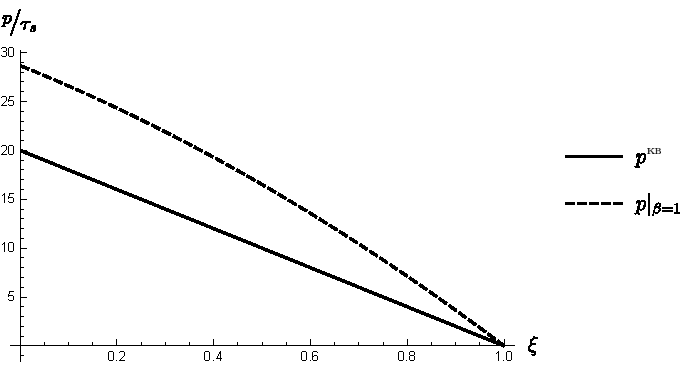
\includegraphics[scale=1.3]{./ch2/pressure_sub3}
    }
    \caption{Эпюры давления для случая цилиндрического слоя при радиусах ``промежуточного'' порядка}
    \label{fig:ch2/sec7/pressure}
\end{figure}


Пользуясь тем, что в случае $c\in\left(0,1\right)$ имеет место равенство $\mathcal{V}_0 / \pi~=~\left(2a \alpha^{c} + \alpha\right) h^{3} / \alpha^{2}$, где $\mathcal{V}_0$ -- объем слоя, а высота слоя $h$ представима в виде $h=V \left(t_*-t\right)$, можно установить зависимость между временем и стадией прессования:
\begin{equation}
  t_* - t \sim \frac{\text{Eu}^{\nicefrac{-1}{3\beta}}}{V}\sqrt[3]{\frac{\mathcal{V}_0}{\pi(2a\text{Eu}^{\nicefrac{(1-c)}{3\beta}}+1)}}
\end{equation}
           % Глава 2
\chapter{Задача о сдавливании сферического идеально жесткопластического слоя}\label{ch:ch3}
На основе анализа классической задачи Прандтля \autocite{Prandtl:1948} получены значительные результаты связанные с теорией течение по поверхностям, которые имеют широкое применение для решения технологических задач. Одним из обобщений данной задачи является случай осесимметричного меридионального течение со стоком между двумя концентрическими шероховатыми сферами \autocite{Georgievsky:2011}.
Решение данной задачи применимо в различных технологиях изготовления тонких сферических тел, например в штамповке взрывом.
% \fixme{Сформулировать мысль про применение в каком-нибудь процессе формообразования, например в штамповке взрывом.} 
В данной постановке задачи исследуется влияние динамических эффектов в процессе формирования изделия методом прессования. Материалы главы содержатся в публикации \autocite{Shabaykin:2020a}.

\section{Постановка задачи и асимптотические разложения}\label{sec:ch3/sec1}

Пренебрегая начальными упругими деформациями, вязкостью и незначительным упрочнением, материал, имеющий плотность $\varrho$, полагается несжимаемым идеально жесткопластическим, удовлетворяющим тензорно линейным определяющим соотношениям и скалярному определяющему соотношению -- квадратичному критерию Мизеса-Генки $\sigma_{u} = \sigma_{s}$, где $\sigma_{u} = \sqrt{\utilde{s} : \utilde{s}}$ -- интенсивность напряжения, $\utilde{s}$ -- девиатор напряжения, $\sigma_{s}$ -- предел текучести.

Пусть течение происходит в области
\begin{equation}
  \Omega_{t} = \{0 \le r \le R(t)+ h(t), 0 \le \theta < \pi, 0 \le \phi < 2\pi\},
\end{equation}
с границей $\partial\Omega = \Gamma = \Gamma_{1} \cup \Gamma_{2}$, причем $h(t) \ll R(t)$ для любого $t \ge 0$.

Внешняя сфера неподвижна, а внутренняя радиально расширяется с постоянной скоростью, выдавливая материал через сток $\theta=\pi$.

\begin{figure}[ht]
  \centerfloat{
    \includegraphics[width=0.6\linewidth]{./ch3/layer}
  }
  \caption{Представление сферического слоя}
  \label{fig:ch3/layer/circle}
\end{figure}
Скорость расширения внутренней сферы обозначим $V$, поэтому кинематическое условие непротекания сквозь границы $\Gamma_{1}$ и $\Gamma_{2}$ имеет вид
\begin{equation}
  \label{eq:ch3/sec1/boundary/kinematic}
  v_{r}\lvert_{r=R} = V, \quad v_{r}\lvert_{r=R + h} = 0
\end{equation}
Касательная составляющая скорости (в данном случае $v_{\theta}$) на указанных границах идеальной среды, как известно, не задаётся.

В некоторый момент времени $0 < t <  h_{0}/V = t_*$, где $t_*$ -- момент схлопывания слоя, относительно шести функций -- независимых компонент девиатора напряжений $s_{rr}$, $s_{r\theta}$ и $s_{\theta\theta}$, давления $p$ и компонент скорости $v_{r}$ и $v_{\theta}$ -- должна выполнятся замкнутая система уравнений динамической теории идеальной пластичности для цилиндрических координат:
\begin{subequations}
  \label{eqs:ch3/sec1/general}
  \begin{gather}
    \label{eqs:ch3/sec1/general/motion:1}
    \begin{multlined}
      -p_{,r}+s_{rr,r}+\frac{1}{r}\left(s_{r\theta,\theta}+3s_{rr}+s_{r\theta}\cot{\left(\theta\right)}\right) \unl{=}
      \varrho \left(v_{r;t}+v_{r} v_{r,r} + \frac{1}{r}v_{\theta} v_{r,\theta} - \frac{1}{r} v_{\theta}^2 \right)
    \end{multlined}
    \\
    \label{eqs:ch3/sec1/general/motion:2}
    \begin{multlined}
      -\frac{1}{r} p_{,\theta}+s_{r\theta,r}+\frac{1}{r}\left(s_{\theta\theta,\theta}+3s_{r\theta}+\left(s_{rr}+2s_{\theta\theta}\right)\cot{\left(\theta\right)}\right) \unl{=}
      \varrho \left(v_{\theta;t}+v_{r} v_{\theta,r} + \frac{1}{r}v_{\theta} v_{\theta,\theta} - \frac{1}{r} v_{\theta} v_{r} \right)
    \end{multlined}
    \\
    \label{eqs:ch3/sec1/general/plasticity}
    s^2_{rr}+s^2_{\theta\theta}+s_{rr} s_{\theta\theta} + s^2_{r\theta}=\tau^2_{s}
    \\
    \label{eqs:ch3/sec1/general/coax:1}
    s_{rr} \left(v_{\theta,\theta} + v_{r}\right) / r = s_{\theta\theta} v_{r,r}
    \\
    \label{eqs:ch3/sec1/general/coax:2}
    s_{rr} \left(v_{\theta,r}+\left(v_{r,\theta}-v_{\theta}\right) / r\right) = 2 s_{r\theta} v_{r,r}
    \\
    \label{eqs:ch3/sec1/general/uncompress}
    v_{r,r}+\left(2v_{r}+v_{\theta,\theta}+v_{\theta}\cot{\left(\theta\right)}\right) / r = 0
  \end{gather}
\end{subequations}
Кроме выполнения условия \cref{eq:ch3/sec1/boundary/kinematic} на жестких контактирующих поверхностях потербуем, что бы модуль касательного напряжения $s_{r\theta}$ достигал на границах $\Gamma_{1}$ и $\Gamma_{2}$ своего максимального значения:
\begin{equation}
  \label{eq:ch3/sec1/boundary/force}
  \lvert s_{r\theta}\lvert_{r=R} = \lvert s_{r\theta}\lvert_{r=R+h} = \mu(\theta) \tau_{s}, \quad 0 < \mu \le 1,
\end{equation}
где $\mu$ -- шероховатость пресса. Абсолютной шероховатости, или полному сцеплению пресса с материалом, соответствует значение $\mu = 1$.


Введем малый параметр $\alpha = \frac{h(t)}{R(t)} \ll 1$ и проведем разложение всех неизвестных величин, входящих в систему уравнений \cref{eqs:ch3/sec1/general}, в ряды по целым степеням параметра:
\begin{subequations}
  \label{eqs:ch3/series}
  \begin{gather}
    v_{\theta}\left(r, \theta, t\right) = V \sum_{k=-N}^{\infty}{\alpha^{k} \; \uindex{v}{k}_{\theta}}, \quad N \ge 1
    \\
    v_{r}\left(r, \theta, t\right) = V \sum_{k=0}^{\infty}{\alpha^{k} \; \uindex{v}{k}_{r}}
    \\
    s_{ij}\left(r, \theta, t\right) = \tau_{s} \sum_{k=0}^{\infty}{\alpha^{k} \; \uindex{s}{k}_{ij}}, \quad (ij)\in\{rr, r\theta, \theta\theta\}
    \\
    p\left(r, \theta, t \right) = \tau_{s} \sum_{k=-M}^{\infty}{\alpha^{k} \; \uindex{p}{k}}, \quad M \ge 1
  \end{gather}
\end{subequations}
Коэффициенты рядов \cref{eqs:ch3/series} -- безразмерны и являются функциями безразмерных координат $\rho, \theta, \tau$ :
\begin{equation}
  \label{eq:ch3/coordinates}
  \rho = \frac{r-R}{h}, \quad \tau = V \frac{t}{h}
\end{equation}
Наличие в \cref{eqs:ch3/series} членов $\alpha^{-n} \; \uindex{v}{-n}_{\theta}$ и $\alpha^{-m} \; \uindex{p}{-m}$ обусловлено стремлением $v_{r}$ и $p$ к бесконечности, при $\alpha\rightarrow 0$, что ясно из физических соображений.
Используя равенство $\dot{R}=-\dot{h}= V$ выразим малый параметр и координаты \cref{eq:ch3/coordinates} как эволюционные функции:
\begin{subequations}
  \begin{gather}
    \dot{\alpha} = \left(\frac{h}{R}\right)^. = \frac{\dot{h}R - h\dot{R}}{h^2} = -\frac{V}{h} \alpha \left(1+\alpha\right)
    \\
    \dot{\rho} = \left(\frac{r-R}{h}\right)^. = \frac{\dot{R} h - \left(r-R\right) \dot{h}}{h^2} = -\frac{V}{h}\left(1-\rho\right)
    \\
    \dot{\tau} = \left(V \frac{t}{h}\right)^. = V \frac{h - t\dot{h}}{h^2} = \frac{V}{h} \left(1+\tau\right)
  \end{gather}
\end{subequations}
Подставляя выражения \cref{eqs:ch3/series} в систему \cref{eqs:ch3/sec1/general} и учитывая, что полная производная по времени представляется в виде
\begin{equation*}
  \uindex{v}{k}_{i;t} = \uindex{v}{k}_{i,\rho} \dot{\rho} + \uindex{v}{k}_{i,\tau} \dot{\tau}
\end{equation*}
получим следующую систему:
\begingroup
\allowdisplaybreaks
\begin{subequations}
  \label{eqs:ch3/sec1/substituted}
  \begin{gather}
    \label{eqs:ch3/sec1/substituted/motion:1}
    \begin{multlined}
      -\!\!\!\!\sum_{k=-M}^{\infty}{\!\!\alpha^{k} \; \uindex{p}{k}_{,\rho}}{+}\sum_{k=0}^{\infty}{\alpha^{k} \; \uindex{s}{k}_{rr,\rho}}{+}
      \frac{\alpha}{1{+}\alpha\rho} \sum_{k=0}^{\infty}\alpha^{k} \left(\ \uindex{s}{k}_{r\theta,\theta} + 3\ \uindex{s}{k}_{rr} + \uindex{s}{k}_{r\theta}\cot{\left(\theta\right)}\right) \unl{=} \frac{\varrho V^2}{\tau_{s}}\left( \vphantom{\left(\sum_{k=-N}^{\infty}\right)^2}
      \sum_{k=0}^{\infty}\alpha^{k} \left(\;
      \left(1-\rho\right)\uindex{v}{k}_{r,\rho} + \uindex{v}{k}_{r,\theta} + \left(1+\tau\right)\uindex{v}{k}_{r,\tau} - \left(1+\alpha\right)\uindex{v}{k}_{r}
      \right) \unl[1]{+}
      \sum_{k=0}^{\infty}{\alpha^{k} \; \uindex{v}{k}_{r}} \sum_{k=0}^{\infty}{\alpha^{k} \; \uindex{v}{k}_{r,\rho}} {+} \frac{\alpha}{1{+}\alpha\rho} \left( \vphantom{\left(\sum_{k=-N}^{\infty}\right)^2}
      \sum_{k=-N}^{\infty}{\alpha^{k} \; \uindex{v}{k}_{\theta}} \sum_{k=0}^{\infty}{\alpha^{k} \; \uindex{v}{k}_{r,\theta}} \unl[2]{-}
      \left(\sum_{k=-N}^{\infty}{\alpha^{k} \; \uindex{v}{k}_{\theta}}\right)^2
      \right)
      \right)
    \end{multlined}
    \\
    \label{eqs:ch3/sec1/substituted/motion:2}
    \begin{multlined}
      -\frac{\alpha}{1+\alpha\rho}\sum_{k=-M}^{\infty}{\alpha^{k} \; \uindex{p}{k}_{,\theta}}+\sum_{k=0}^{\infty}{\alpha^{k} \; \uindex{s}{k}_{r\theta,\rho}}+
      \frac{\alpha}{1+\alpha\rho} \sum_{k=0}^{\infty}\alpha^{k} \left(\ \uindex{s}{k}_{\theta\theta,\theta} + 3\ \uindex{s}{k}_{r\theta} \unl[1]{+}
      \left(\ \uindex{s}{k}_{rr}+2\uindex{s}{k}_{\theta\theta}\right)\cot{\left(\theta\right)}\right) \unl{=}
      \frac{\varrho V^2}{\tau_{s}}\left(
      \sum_{k=-N}^{\infty}\alpha^{k} \left(\;
      \left(1-\rho\right)\uindex{v}{k}_{\theta,\rho} + \uindex{v}{k}_{\theta,\theta} + \left(1+\tau\right)\uindex{v}{k}_{\theta,\tau} - \left(1+\alpha\right)\uindex{v}{k}_{\theta}
      \right) \unl[1]{+}
      \sum_{k=0}^{\infty}{\alpha^{k} \; \uindex{v}{k}_{r}} \sum_{k=-N}^{\infty}{\alpha^{k} \; \uindex{v}{k}_{\theta,\rho}} {+} \frac{\alpha}{1{+}\alpha\rho} \left( \vphantom{\left(\sum_{k=-N}^{\infty}\right)^2}
      \sum_{k=-N}^{\infty}{\alpha^{k} \; \uindex{v}{k}_{\theta}} \sum_{k=0}^{\infty}{\alpha^{k} \; \uindex{v}{k}_{r,\theta}} \unl[2]{-}
      \sum_{k=-N}^{\infty}{\alpha^{k} \; \uindex{v}{k}_{\theta}} \sum_{k=0}^{\infty}{\alpha^{k} \; \uindex{v}{k}_{r}}
      \right)
      \right)
    \end{multlined}
    \\
    \label{eqs:ch3/sec1/substituted/plasticity}
    \begin{multlined}
      \left(\sum_{k=0}^{\infty}{\alpha^{k} \; \uindex{s}{k}_{rr}}\right)^2+
      \left(\sum_{k=0}^{\infty}{\alpha^{k} \; \uindex{s}{k}_{\theta\theta}}\right)\unl{+}
      \sum_{k=0}^{\infty}{\alpha^{k} \; \uindex{s}{k}_{rr}} \sum_{k=0}^{\infty}{\alpha^{k} \; \uindex{s}{k}_{\theta\theta}}+
      \left(\sum_{k=0}^{\infty}{\alpha^{k} \; \uindex{s}{k}_{r\theta}}\right)^2 = 1
    \end{multlined}
    \\
    \label{eqs:ch3/sec1/substituted/coax:1}
    \sum_{k=0}^{\infty}{\alpha^{k} \; \uindex{s}{k}_{rr}} \; \frac{\alpha}{1{+}\alpha\rho} \left(\sum_{k=-N}^{\infty}{\alpha^{k} \; \uindex{v}{k}_{\theta,\theta}} + \sum_{k=0}^{\infty}{\alpha^{k} \; \uindex{v}{k}_{r}}\right) = \sum_{k=0}^{\infty}{\alpha^{k} \; \uindex{s}{k}_{\theta\theta}} \sum_{k=0}^{\infty}{\alpha^{k} \; \uindex{v}{k}_{r,\rho}}
    \\
    \label{eqs:ch3/sec1/substituted/coax:2}
    \sum_{k=0}^{\infty}{\alpha^{k} \; \uindex{s}{k}_{rr}} \left(
    \sum_{k=-N}^{\infty}{\alpha^{k} \; \uindex{v}{k}_{\theta,\rho}} + \frac{\alpha}{1+\alpha\rho}\left(\sum_{k=0}^{\infty}{\alpha^{k} \; \uindex{v}{k}_{r,\theta}} - \sum_{k=-N}^{\infty}{\alpha^{k} \; \uindex{v}{k}_{\theta}}\right)
    \right) \unl{=} 2 \sum_{k=0}^{\infty}{\alpha^{k} \; \uindex{s}{k}_{r\theta}} \sum_{k=0}^{\infty}{\alpha^{k} \; \uindex{v}{k}_{r,\rho}}
    \\
    \label{eqs:ch3/sec1/substituted/uncompress}
    \sum_{k=0}^{\infty}{\alpha^{k} \; \uindex{v}{k}_{r,\rho}} + \frac{\alpha}{1+\alpha\rho}\left(
    2 \sum_{k=0}^{\infty}{\alpha^{k} \; \uindex{v}{k}_{r}} + \sum_{k=-N}^{\infty}{\alpha^{k} \left(\ \uindex{v}{k}_{\theta,\theta} + \uindex{v}{k}_{\theta}\cot{\left(\theta\right)}\right)}
    \right) = 0
  \end{gather}
\end{subequations}
\endgroup
Возникший в правой части уравнений \cref{eqs:ch3/sec1/substituted/motion:1, eqs:ch3/sec1/substituted/motion:2} коэффициент равен обратному числу Эйлера
\begin{equation*}
  \text{Eu}^{-1} = \frac{\varrho V^2}{\tau_{s}}.
\end{equation*}
Данная величина мала \todo{почему?}и как видно из её определения фиксирована. По сравнению с ней порядок малости $\alpha(t)$ при течении времени от 0 до $t_*$ растёт до бесконечности. Это позволяет записать
\begin{equation*}
  \text{Eu}^{-1} = O\left(\alpha^\beta(t)\right), \text{ причем } \beta \rightarrow 0 \text{ при } t \rightarrow t_*
\end{equation*}
Применительно к динамическому анализу интерес представляет $0 < \beta \le 2$. Отыскание решений проведем для целочисленных значений входящих в этот диапазон.

Обратимся к системе двух уравнений \cref{eqs:ch3/sec1/substituted/coax:1, eqs:ch3/sec1/substituted/coax:2}. Принимая во внимание малость параметра $\alpha$ и пользуясь разложением в ряд Тейлора
\begin{equation*}
  \frac{1}{1+\alpha\rho} = \sum_{k=0}^{\infty}{\left(-\alpha\rho\right)^k}
\end{equation*}
из \cref{eqs:ch3/sec1/substituted/coax:1} получаем, что $\uindex{v}{-N}_{\theta,\theta} = 0$, а из уравнения \cref{eqs:ch3/sec1/substituted/coax:2} следует $\uindex{v}{-N}_{\theta,\rho} = 0$. Таким образом $\uindex{v}{-N}_{\theta} = \const$, и, исключая вращение слоя как твердого тела, окончательно получаем, что $\uindex{v}{-N}_{\theta} = 0$. Аналогичные рассуждения применимы последовательно для $\uindex{v}{-N+1}_{\theta}$, затем $\uindex{v}{-N+2}_{\theta}$ и далее вплоть до $\uindex{v}{-2}_{\theta}$.
Учитывая, что первый ненулевой член компоненты скорости $\uindex{v}{-1}_{\theta}$, и принимая, что $\beta \ge 1$ определим из уравнений \cref{eqs:ch3/sec1/substituted/motion:1, eqs:ch3/sec1/substituted/motion:2} порядок малости для функции давления $p$. Для $M \ge 2$ имеем:
\begin{equation*}
  -\uindex{p}{-M}_{,\rho} = 0, \quad -\uindex{p}{-M}_{,\theta} = 0 \text{ и, следовательно, } \ \uindex{p}{-M} = \uindex{p}{-M}_{0}(\tau)
\end{equation*}
Здесь $\uindex{p}{-M}_{0}$ -- гидростатическая постоянная, не дающая вклад в уравнение движения и однозначно определяемая заданием внешнего давления. Поэтому, без ограничения общности, можно считать, что $M=1$.

\section{Построение решения}\label{sec:ch3/sec2}
\subsection{Переход от квазистатического к динамическому режиму деформирования}\label{subsec:ch3/sec2/sub1}

Рассмотрим случай $\beta=2$, который соответствует моменту перехода от квазистатического к динамическому режиму деформирования.

Положим $\text{Eu}^{-1} = C_2 \alpha^2$ и последовательно приравняем коэффициенты правых и левых частей уравнений системы \cref{eqs:ch3/sec1/substituted} при $a^{-1}$ и $\alpha^0$:
\begin{subequations}
  \label{eqs:ch3/sec2/sub1/main}
  \begin{gather}
    \label{eqs:ch3/sec2/sub1/-1/motion:1}
    -\uindex{p}{-1}_{,\rho} = 0
    \\
    \label{eqs:ch3/sec2/sub1/-1/coax:2}
    \uindex{s}{0}_{rr} \; \uindex{v}{-1}_{\theta,\rho} = 0
    \\
    \label{eqs:ch3/sec2/sub1/0/motion:1}
    -\uindex{p}{0}_{,\rho} + \uindex{s}{0}_{rr,\rho} = 0
    \\
    \label{eqs:ch3/sec2/sub1/0/motion:2}
    -\uindex{p}{-1}_{,\theta} + \uindex{s}{0}_{r\theta,\rho} = 0
    \\
    \label{eqs:ch3/sec2/sub1/0/plasticity}
    \left(\uindex{s}{0}_{rr}\right)^2 + \left(\uindex{s}{0}_{\theta\theta}\right)^2 + \uindex{s}{0}_{rr}\; \uindex{s}{0}_{\theta\theta} + \left(\uindex{s}{0}_{r\theta}\right)^2 = 1
    \\
    \label{eqs:ch3/sec2/sub1/0/coax:1}
    \uindex{s}{0}_{rr} \; \uindex{v}{-1}_{\theta,\theta} = \uindex{s}{0}_{\theta\theta} \uindex{v}{0}_{r,\rho}
    \\
    \label{eqs:ch3/sec2/sub1/0/coax:2}
    \uindex{s}{0}_{rr} \left(\ \uindex{v}{0}_{\theta,\rho} - \uindex{v}{-1}_{\theta}\right) = 2 \uindex{s}{0}_{r\theta} \; \uindex{v}{0}_{r,\rho}
    \\
    \label{eqs:ch3/sec2/sub1/0/uncompress}
    \uindex{v}{0}_{r,\rho} + \uindex{v}{-1}_{\theta,\theta} + \uindex{v}{-1}_{\theta} \cot{\left(\theta\right)} = 0
  \end{gather}
\end{subequations}
Граничные условия \cref{eq:ch3/sec1/boundary/kinematic, eq:ch3/sec1/boundary/force} при этом примут вид
\begin{equation}
  \label{eq:ch3/sec2/sub1/boundary/0}
  \uindex{v}{0}_{r}\lvert_{\rho=0} = 1, \quad \uindex{v}{0}_{r}\lvert_{\rho=1} = 0, \quad \lvert \uindex{s}{0}_{r\theta}\lvert_{\rho=0} = \lvert \uindex{s}{0}_{r\theta}\lvert_{\rho=1} = \mu(\theta)
\end{equation}
Из уравнений \cref{eqs:ch3/sec2/sub1/-1/motion:1, eqs:ch3/sec2/sub1/-1/coax:2} вытекает
\begin{equation*}
  \uindex{p}{-1} = \uindex{f}{-1}_{p}(\theta, \tau), \quad \uindex{v}{-1}_{\theta} = \uindex{f}{-1}_{v_{\theta}}(\theta, \tau).
\end{equation*}
Подставив выражение $\uindex{v}{-1}_{r}$ в уравнение \cref{eqs:ch3/sec2/sub1/0/uncompress} и решив дифференциальное уравнение, получим выражение для $\uindex{v}{0}_{r}$:
\begin{equation*}
  \uindex{v}{0}_{r} = \uindex{f}{0}_{v_{r}}(\rho, \tau) -\rho \left(\ \uindex{f}{-1}_{v_{\theta},\theta} + \uindex{f}{-1}_{v_{\theta}} \cot{\left(\theta\right)}\right)
\end{equation*}
Подстановка данного равенства в кинематические граничные условия \cref{eq:ch3/sec2/sub1/boundary/0} и использование их линейной комбинации позволяет определить неизвестные функции интегрирования:
\begin{gather*}
  \uindex{f}{0}_{v_{z}} = 1
  \\
  \uindex{f}{-1}_{v_{\theta},\theta} + \uindex{f}{-1}_{v_{\theta}} \cot{\left(\theta\right)} = 1
  \\
  \uindex{f}{-1}_{v_{\theta}} = -\cot{\left(\theta\right)} + \frac{\uindex{g}{-1}_{v_{\theta}}\left(\tau\right)}{\sin{\left(\theta\right)}}
\end{gather*}
В силу требования ограниченности членов разложения, следует положить $\uindex{g}{-1}_{v_{\theta}}~=~1$. Окончательно получаем
\begin{gather}
  \label{sol:ch3/sec2/sub1/vt/-1}
  \uindex{v}{-1}_{\theta} = \uindex{f}{-1}_{v_{\theta}} = -\cot{\left(\theta\right)} + \frac{1}{\sin{\left(\theta\right)}} = \tan{\left({\theta / 2}\right)}
  \\
  \label{sol:ch3/sec2/sub1/vr/0}
  \uindex{v}{0}_{r} =  1-\rho
\end{gather}
Решая \cref{eqs:ch3/sec2/sub1/0/motion:2} относительно $\uindex{s}{0}_{r\theta}$ и используя силовые граничные условия \cref{eq:ch3/sec2/sub1/boundary/0} придем к
\begin{gather*}
  \uindex{s}{0}_{r\theta} = \uindex{f}{0}_{s_{r\theta}}(\theta, \tau) + \rho  \uindex{f}{-1}_{p,\theta}
  \\
  \uindex{f}{0}_{s_{r\theta}} = \mu\hat{s}, \quad \hat{s} = \pm 1
  \\
  \mu\hat{s} + \uindex{f}{-1}_{p,\xi} = -\mu \hat{s}
  \\
  \uindex{p}{-1}=\uindex{f}{-1}_{p} =\uindex{g}{-1}_{p}(\tau) -2\hat{s}\int_0^{\theta}{\mu(\xi)d\xi}
\end{gather*}
В соответствии с физико-механическим смыслом процесса сжатия и растекания слоя сингулярная составляющая давления $\uindex{p}{-1}$ максимальна в центре слоя, то есть в окрестности $\theta = 0$ , и убывает при движении к границе $\theta=\pi$. Данное обстоятельство позволяет определить, что $\hat{s} = 1$ и тогда окончательно имеем
\begin{gather}
  \label{sol:ch3/sec2/sub1/srt/0}
  \uindex{s}{0}_{r\theta} = -\mu\left(2\rho-1\right)
  \\
  \label{sol:ch3/sec2/sub1/p/-1}
  \uindex{p}{-1} = \uindex{g}{-1}_{p}(\tau) -2\int_0^{\theta}{\mu(\xi)d\xi}
\end{gather}
С учетом найденных функций \cref{eqs:ch3/sec2/sub1/0/coax:1, eqs:ch3/sec2/sub1/0/plasticity} представляют собой алгебраическую систему уравнений относительно $\uindex{s}{0}_{rr}$ и $\uindex{s}{0}_{\theta\theta}$, решив которую, найдем
\begin{gather}
  \label{sol:ch3/sec2/sub1/srr/0}
  \uindex{s}{0}_{rr} = -\frac{\sin^2{\left(\theta\right)}\sqrt{1-\mu^2\left(2\rho-1\right)^2}}{\sqrt{1-\cos{\left(\theta\right)}}\sqrt{1-\cos^3{\left(\theta\right)}}}
  \\
  \label{sol:ch3/sec2/sub1/stt/0}
  \uindex{s}{0}_{\theta\theta} = \frac{\sqrt{1-\cos{\left(\theta\right)}}}{\sqrt{1-\cos^3{\left(\theta\right)}}}\sqrt{1-\mu^2\left(2\rho-1\right)^2}
\end{gather}
Выбор знака в \cref{sol:ch3/sec2/sub1/srr/0,sol:ch3/sec2/sub1/stt/0} обусловлен тем, что в процессе сжатия компонента $s_{rr}$ девиатора напряжений в главном по $\alpha$ приближении всюда в слое должна быть отрицательна. Тогда кольцевая компонента $\uindex{s}{0}_{\theta\theta}$ всюду положительна, а микропрофиль осевой скорости $\uindex{v}{0}_{\theta}$ по толщине будет выпуклым в направлении движения частиц. Подставив все найденные функции в \cref{eqs:ch3/sec2/sub1/0/motion:1, eqs:ch3/sec2/sub1/0/coax:2} и решив дифференциальные уравнения найдем:
\begin{gather}
  \label{sol:ch3/sec2/sub1/vt/0}
  \begin{multlined}
    \uindex{v}{0}_{\theta} = \rho \tan{\left({\theta / 2}\right)} + \frac{\sqrt{1-\cos{\left(\theta\right)}}\sqrt{1-\cos^3{\left(\theta\right)}}}{\mu \sin^2{\left(\theta\right)}}
    \sqrt{1-\mu^2\left(2\rho-1\right)^2} \unl{+} \uindex{f}{0}_{v_{\theta}}(\theta,\tau)
  \end{multlined}
  \\
  \label{sol:ch3/sec2/sub1/p/0}
  \uindex{p}{0} = \uindex{s}{0}_{rr} +\uindex{f}{0}_{p}(\theta,\tau)
\end{gather}
Для нахождение неизвестных функций $\uindex{f}{0}_{p}$ и $\uindex{f}{0}_{v_{\theta}}$ выпишем следующее по $\alpha$ приближение уравнений \cref{eqs:ch3/sec1/substituted/motion:2, eqs:ch3/sec1/substituted/uncompress}, а также граничные условия \cref{eq:ch3/sec1/boundary/kinematic, eq:ch3/sec1/boundary/force}:
\begin{subequations}
  \begin{gather}
    \label{eqs:ch3/sec2/sub1/1/motion:2}
    \begin{multlined}
      -\uindex{p}{0}_{,\theta} +\rho \ \uindex{p}{-1}_{,\theta} + \uindex{s}{1}_{r\theta,\rho} + \uindex{s}{0}_{\theta\theta,\theta} + 3 \ \uindex{s}{0}_{r\theta} \unl{+}
      \left(\uindex{s}{0}_{rr} + 2 \ \uindex{s}{0}_{\theta\theta}\right) \cot{\left(\theta\right)} = C_2 \left(\ \uindex{v}{-1}_{\theta} + \uindex{v}{-1}_{\theta} \; \uindex{v}{-1}_{\theta,\theta}\right)
    \end{multlined}
    \\
    \label{eqs:ch3/sec2/sub1/1/uncompress}
    \uindex{v}{1}_{r,\rho} + 2 \ \uindex{v}{0}_{r} + \uindex{v}{0}_{\theta,\theta} - \rho \; \uindex{v}{-1}_{\theta,\theta}
    + \left(\uindex{v}{0}_{\theta} - \rho \; \uindex{v}{-1}_{\theta}\right) \cot{\left(\theta\right)}= 0
    \\
    \label{eq:ch3/sec2/sub1/boundary/1}
    \uindex{v}{1}_{r}\lvert_{\rho=0}= \uindex{v}{1}_{r}\lvert_{\rho=1} = 0, \quad \lvert \uindex{s}{1}_{r\theta}\lvert_{\rho=0} = \uindex{s}{1}_{r\theta}\lvert_{\rho=1} = 0
  \end{gather}
\end{subequations}
Функция $\uindex{v}{1}_{r}$ является непрерывной, поэтому имеет место равенство
\begin{equation}
  \label{eq:ch3/sec2/sub1/interm/1}
  \begin{multlined}
    0 = \uindex{v}{1}_{r}\lvert_{\rho= 1} - \uindex{v}{1}_{r}\lvert_{\rho=0} = \int_{0}^{1}{\uindex{v}{1}_{r,\rho}d\rho} \unl{=}
    -\int_{0}^{1}{\left( 2 \ \uindex{v}{0}_{r} + \uindex{v}{0}_{\theta,\theta} - \rho \; \uindex{v}{-1}_{\theta,\theta}
    + \left(\uindex{v}{0}_{\theta} - \rho \; \uindex{v}{-1}_{\theta}\right) \cot{\left(\theta\right)}\right) d\rho}
  \end{multlined}
\end{equation}
Введем обозначение
\begin{equation*}
  \begin{multlined}
    \zeta = \int_{0}^{1}{\left(\uindex{v}{0}_{\theta} - \rho \; \uindex{v}{-1}_{\theta}\right) d\rho} \unl{=} \frac{\sqrt{1-\cos{\left(\theta\right)}}\sqrt{1-\cos^3{\left(\theta\right)}}}{\mu \sin^2{\left(\theta\right)}}
    \left(\arcsin\left(\mu\right) + \mu \sqrt{1-\mu^2}\right) + \uindex{f}{0}_{v_{\theta}}(\theta,\tau)
  \end{multlined}
\end{equation*}
Тогда выражение \cref{eq:ch3/sec2/sub1/interm/1} перепишется в виде
\begin{equation*}
  1+\zeta_{,\theta}+\zeta \cot{\left(\theta\right)} = 0,
\end{equation*}
Его решением будет
\begin{equation*}
  \zeta = \cot{\left(\theta\right)} + \frac{g_{\zeta}\left(\tau\right)}{\sin{\left(\theta\right)}}
\end{equation*}
В силу требования ограниченности членов разложения, следует положить $g_{\zeta}~=~1$. Таким образом получаем выражение для $\uindex{f}{0}_{v_{\theta}}$:
\begin{equation}
  \uindex{f}{0}_{v_{\theta}} = -\frac{\sqrt{1-\cos{\left(\theta\right)}}\sqrt{1-\cos^3{\left(\theta\right)}}}{\mu \sin^2{\left(\theta\right)}}
  \left(\arcsin\left(\mu\right) + \mu \sqrt{1-\mu^2}\right)
  -\tan{\left({\theta / 2}\right)}
\end{equation}
Аналогичные операции проведем над функцией $\uindex{s}{1}_{r\theta}$:
\begin{equation}
  \label{eq:ch3/sec2/sub1/interm/2}
  \begin{multlined}
    0 = \uindex{s}{1}_{r\theta}\lvert_{\rho= 1} - \uindex{s}{1}_{r\theta}\lvert_{\rho=0} = \int_{0}^{1}{\uindex{s}{1}_{r\theta,\rho}d\rho} \unl{=}
    -\int_{0}^{1}\left(
    -\uindex{f}{0}_{p,\theta} - \uindex{s}{0}_{rr,\theta} + \uindex{s}{0}_{\theta\theta,\theta} + 2\rho \mu  + 3 \ \uindex{s}{0}_{r\theta} \unl[1]{+}
    \left(\uindex{s}{0}_{rr} + 2 \ \uindex{s}{0}_{\theta\theta}\right) \cot{\left(\theta\right)} - C_2 \left(\ \uindex{v}{-1}_{\theta} + \uindex{v}{-1}_{\theta} \; \uindex{v}{-1}_{\theta,\theta}\right) \vphantom{\uindex{f}{0}_{p}}
    \right) d\rho \unl{=}
    -\uindex{f}{0}_{p,\theta} + \mu -C_2 \left(1+\frac{1}{1+\cos{\left(\theta\right)}}\right)\tan{\left({\theta / 2}\right)} \unl{+}
    %\frac{\arcsin\left(\mu\right) + \mu \sqrt{1-\mu^2}}{\sqrt{1-\mu^2\left(2\rho-1\right)^2}}
    \int_{0}^{1} \left(
    \uindex{s}{0}_{\theta\theta,\theta} - \uindex{s}{0}_{rr,\theta} + \left(\uindex{s}{0}_{rr} + 2 \ \uindex{s}{0}_{\theta\theta}\right) \cot{\left(\theta\right)}
    \right) d\rho = 0
  \end{multlined}
\end{equation}
Пользуясь тем, что $\uindex{s}{0}_{aa} = K_{aa}(\theta) \sqrt{1-\mu^2\left(2\rho-1\right)^2}$, выразим интегралы от диагональных компонент девиатора напряжений:
\begin{equation*}
  \int_{0}^{1} \uindex{s}{0}_{aa} d\rho = K_{aa}(\theta) \left(\arcsin\left(\mu\right) + \mu \sqrt{1-\mu^2}\right)
  = \frac{\arcsin\left(\mu\right) + \mu \sqrt{1-\mu^2}}{\sqrt{1-\mu^2\left(2\rho-1\right)^2}} \ \uindex{s}{0}_{aa}.
\end{equation*}
Окончательно получаем выражение для $\uindex{f}{0}_{p}$:
\begin{equation}
  \begin{multlined}
    \uindex{f}{0}_{p} = \int_0^{\theta}{\mu(\xi)d\xi} + C_2 \left(2\log{\left(\cos{\left({\theta / 2}\right)}\right)} - \frac{1}{1+\cos{\left(\theta\right)}}\right) \unl{+}
    \int \frac{\arcsin\left(\mu\right) + \mu \sqrt{1-\mu^2}}{\sqrt{1-\mu^2\left(2\rho-1\right)^2}}\left(
    \uindex{s}{0}_{\theta\theta,\theta} - \uindex{s}{0}_{rr,\theta} + \left(\uindex{s}{0}_{rr} + 2 \ \uindex{s}{0}_{\theta\theta}\right) \cot{\left(\theta\right)}
    \right) d\theta \unl{+} \uindex{g}{0}_{p}\left(\tau\right)
  \end{multlined}
\end{equation}

\subsection{Развитый процесс динамического деформирования}\label{subsec:ch3/sec2/sub2}

Рассмотрим случай $\beta=1$, который соответствует моменту с сильным влиянием динамики в процессе сдавливания слоя.

Положим $\text{Eu}^{-1} = C_1 \alpha$ и последовательно приравняем коэффициенты правых и левых частей уравнений системы \cref{eqs:ch3/sec1/substituted} при $a^{-1}$ и $\alpha^0$:
\begin{subequations}
  \label{eqs:ch3/sec2/sub2/main}
  \begin{gather}
    \label{eqs:ch3/sec2/sub2/-1/motion:1}
    -\uindex{p}{-1}_{,\rho} = 0
    \\
    \label{eqs:ch3/sec2/sub2/-1/coax:2}
    \uindex{s}{0}_{rr} \; \uindex{v}{-1}_{\theta,\rho} = 0
    \\
    \label{eqs:ch3/sec2/sub2/0/motion:1}
    -\uindex{p}{0}_{,\rho} + \uindex{s}{0}_{rr,\rho} = C_1 \left(\ \uindex{v}{-1}_{\theta}\right)^2
    \\
    \label{eqs:ch3/sec2/sub2/0/motion:2}
    -\uindex{p}{-1}_{,\theta} + \uindex{s}{0}_{r\theta,\rho} = C_1 \left(\ \uindex{v}{-1}_{\theta} + \uindex{v}{-1}_{\theta} \; \uindex{v}{-1}_{\theta,\theta} +
    \left(1+\tau\right) \uindex{v}{-1}_{\theta,\tau}\right)
    \\
    \label{eqs:ch3/sec2/sub2/0/plasticity}
    \left(\uindex{s}{0}_{rr}\right)^2 + \left(\uindex{s}{0}_{\theta\theta}\right)^2 + \uindex{s}{0}_{rr}\; \uindex{s}{0}_{\theta\theta} + \left(\uindex{s}{0}_{r\theta}\right)^2 = 1
    \\
    \label{eqs:ch3/sec2/sub2/0/coax:1}
    \uindex{s}{0}_{rr} \; \uindex{v}{-1}_{\theta,\theta} = \uindex{s}{0}_{\theta\theta} \uindex{v}{0}_{r,\rho}
    \\
    \label{eqs:ch3/sec2/sub2/0/coax:2}
    \uindex{s}{0}_{rr} \left(\ \uindex{v}{0}_{\theta,\rho} - \uindex{v}{-1}_{\theta}\right) = 2 \uindex{s}{0}_{r\theta} \; \uindex{v}{0}_{r,\rho}
    \\
    \label{eqs:ch3/sec2/sub2/0/uncompress}
    \uindex{v}{0}_{r,\rho} + \uindex{v}{-1}_{\theta,\theta} + \uindex{v}{-1}_{\theta} \cot{\left(\theta\right)} = 0
  \end{gather}
\end{subequations}
Как и в предыдущем пункте граничные условия \cref{eq:ch3/sec1/boundary/kinematic, eq:ch3/sec1/boundary/force} примут вид
\begin{equation}
  \label{eq:ch3/sec2/sub2/boundary/0}
  \uindex{v}{0}_{r}\lvert_{\rho=0} = 1, \quad \uindex{v}{0}_{r}\lvert_{\rho=1} = 0, \quad \lvert \uindex{s}{0}_{r\theta}\lvert_{\rho=0} = \lvert \uindex{s}{0}_{r\theta}\lvert_{\rho=1} = \mu(\theta)
\end{equation}
Из уравнений \cref{eqs:ch3/sec2/sub2/-1/motion:1, eqs:ch3/sec2/sub2/-1/coax:2} вытекает
\begin{equation*}
  \uindex{p}{-1} = \uindex{f}{-1}_{p}(\theta, \tau), \quad \uindex{v}{-1}_{\theta} = \uindex{f}{-1}_{v_{\theta}}(\theta, \tau).
\end{equation*}
Подставив выражение $\uindex{v}{-1}_{r}$ в уравнение \cref{eqs:ch3/sec2/sub2/0/uncompress} и решив дифференциальное уравнение, получим выражение для $\uindex{v}{0}_{r}$:
\begin{equation*}
  \uindex{v}{0}_{r} = \uindex{f}{0}_{v_{r}}(\rho, \tau) -\rho \left(\ \uindex{f}{-1}_{v_{\theta},\theta} + \uindex{f}{-1}_{v_{\theta}} \cot{\left(\theta\right)}\right)
\end{equation*}
Подстановка данного равенства в кинематические граничные условия \cref{eq:ch3/sec2/sub2/boundary/0} и использование их линейной комбинации позволяет определить неизвестные функции интегрирования:
\begin{gather*}
  \uindex{f}{0}_{v_{z}} = 1
  \\
  \uindex{f}{-1}_{v_{\theta},\theta} + \uindex{f}{-1}_{v_{\theta}} \cot{\left(\theta\right)} = 1
  \\
  \uindex{f}{-1}_{v_{\theta}} = -\cot{\left(\theta\right)} + \frac{\uindex{g}{-1}_{v_{\theta}}\left(\tau\right)}{\sin{\left(\theta\right)}}
\end{gather*}
Требование ограниченности членов разложения позволяет определить константу интегрирования:
\begin{gather}
  \label{sol:ch3/sec2/sub2/vt/-1}
  \uindex{v}{-1}_{\theta} = \uindex{f}{-1}_{v_{\theta}} = -\cot{\left(\theta\right)} + \frac{1}{\sin{\left(\theta\right)}} = \tan{\left({\theta / 2}\right)}
  \\
  \label{sol:ch3/sec2/sub2/vr/0}
  \uindex{v}{0}_{r} =  1-\rho
\end{gather}
С учетом \cref{sol:ch3/sec2/sub2/vt/-1} уравнение \cref{eqs:ch3/sec2/sub2/0/motion:2} примет вид
\begin{equation*}
  -\uindex{p}{-1}_{,\theta} + \uindex{s}{0}_{r\theta,\rho} = C_1 \left(1+\frac{1}{1+\cos{\left(\theta\right)}}\right) \tan{\left({\theta / 2}\right)}
\end{equation*}
Решая его относительно $\uindex{s}{0}_{r\theta}$ и используя силовые граничные условия \cref{eq:ch3/sec2/sub2/boundary/0} придем к
\begin{gather*}
  \uindex{s}{0}_{r\theta} = \uindex{f}{0}_{s_{r\theta}}(\theta, \tau) + \rho  \uindex{f}{-1}_{p,\theta} \rho C_1 \left(1+\frac{1}{1+\cos{\left(\theta\right)}}\right) \tan{\left({\theta / 2}\right)}
  \\
  \uindex{f}{0}_{s_{r\theta}} = \mu\hat{s}, \quad \hat{s} = \pm 1
  \\
  \mu\hat{s} + \uindex{f}{-1}_{p,\xi} + C_1 \left(1+\frac{1}{1+\cos{\left(\theta\right)}}\right) \tan{\left({\theta / 2}\right)}= -\mu \hat{s}
  \\
  \uindex{p}{-1}=\uindex{f}{-1}_{p} =\uindex{g}{-1}_{p}(\tau) -2\hat{s}\int_0^{\theta}{\mu(\xi)d\xi} + C_1 \left(2\log{\left(\cos{\left({\theta / 2}\right)}\right)} - \frac{1}{1+\cos{\left(\theta\right)}}\right)
\end{gather*}
Аналогично предыдущему пункту следует положить $\hat{s} = 1$, и тогда окончательно имеем
\begin{gather}
  \label{sol:ch3/sec2/sub2/srt/0}
  \uindex{s}{0}_{r\theta} = -\mu\left(2\rho-1\right)
  \\
  \label{sol:ch3/sec2/sub2/p/-1}
  \uindex{p}{-1} = \uindex{g}{-1}_{p}(\tau) -2\int_0^{\theta}{\mu(\xi)d\xi} + C_1 \left(2\log{\left(\cos{\left({\theta / 2}\right)}\right)} - \frac{1}{1+\cos{\left(\theta\right)}}\right)
\end{gather}
С учетом найденных функций \cref{eqs:ch3/sec2/sub2/0/coax:1, eqs:ch3/sec2/sub2/0/plasticity} представляют собой алгебраическую систему уравнений относительно $\uindex{s}{0}_{rr}$ и $\uindex{s}{0}_{\theta\theta}$, решив которую, найдем
\begin{gather}
  \label{sol:ch3/sec2/sub2/srr/0}
  \uindex{s}{0}_{rr} = -\frac{\sin^2{\left(\theta\right)}\sqrt{1-\mu^2\left(2\rho-1\right)^2}}{\sqrt{1-\cos{\left(\theta\right)}}\sqrt{1-\cos^3{\left(\theta\right)}}}
  \\
  \label{sol:ch3/sec2/sub2/stt/0}
  \uindex{s}{0}_{\theta\theta} = \frac{\sqrt{1-\cos{\left(\theta\right)}}}{\sqrt{1-\cos^3{\left(\theta\right)}}}\sqrt{1-\mu^2\left(2\rho-1\right)^2}
\end{gather}
Выбор знака в \cref{sol:ch3/sec2/sub2/srr/0,sol:ch3/sec2/sub2/stt/0} обусловлен тем, что в процессе сжатия компонента $s_{rr}$ девиатора напряжений в главном по $\alpha$ приближении всюда в слое должна быть отрицательна. Тогда кольцевая компонента $\uindex{s}{0}_{\theta\theta}$ всюду положительна, а микропрофиль осевой скорости $\uindex{v}{0}_{\theta}$ по толщине будет выпуклым в направлении движения частиц. Подставив все найденные функции в \cref{eqs:ch3/sec2/sub2/0/motion:1, eqs:ch3/sec2/sub2/0/coax:2} и решив дифференциальные уравнения найдем:
\begin{gather}
  \label{sol:ch3/sec2/sub2/vt/0}
  \begin{multlined}
    \uindex{v}{0}_{\theta} = \rho \tan{\left({\theta / 2}\right)} + \frac{\sqrt{1-\cos{\left(\theta\right)}}\sqrt{1-\cos^3{\left(\theta\right)}}}{\mu \sin^2{\left(\theta\right)}}
    \sqrt{1-\mu^2\left(2\rho-1\right)^2} \unl{+} \uindex{f}{0}_{v_{\theta}}(\theta,\tau)
  \end{multlined}
  \\
  \label{sol:ch3/sec2/sub2/p/0}
  \uindex{p}{0} = \uindex{s}{0}_{rr} - C_1 \rho \tan^2{\left({\theta / 2}\right)} +\uindex{f}{0}_{p}(\theta,\tau)
\end{gather}
Для нахождение неизвестных функций $\uindex{f}{0}_{p}$ и $\uindex{f}{0}_{v_{\theta}}$ выпишем следующее по $\alpha$ приближение уравнений \cref{eqs:ch3/sec1/substituted/motion:2, eqs:ch3/sec1/substituted/uncompress}, а также граничные условия \cref{eq:ch3/sec1/boundary/kinematic, eq:ch3/sec1/boundary/force}:
\begin{subequations}
  \begin{gather}
    \label{eqs:ch3/sec2/sub2/1/motion:2}
    \begin{multlined}
      -\uindex{p}{0}_{,\theta} +\rho \ \uindex{p}{-1}_{,\theta} + \uindex{s}{1}_{r\theta,\rho} + \uindex{s}{0}_{\theta\theta,\theta} + 3 \ \uindex{s}{0}_{r\theta} +
      \left(\uindex{s}{0}_{rr} + 2 \ \uindex{s}{0}_{\theta\theta}\right) \cot{\left(\theta\right)} \unl{=}
      % \uindex{v}{-1}_{\theta} \; \uindex{v}{-1}_{\theta,\theta}
      C_1 \left(\
      \uindex{v}{-1}_{\theta} + \left(\rho-1\right)\uindex{v}{0}_{\theta,\rho} + \left(1 + \tau\right)\uindex{v}{0}_{\theta,\tau} + \uindex{v}{0}_{r} \; \uindex{v}{0}_{\theta,\rho} -
      \rho \ \uindex{v}{-1}_{\theta} \; \uindex{v}{-1}_{\theta,\theta} \unl[1]{+} \uindex{v}{0}_{\theta} \; \uindex{v}{-1}_{\theta,\theta} +
      \uindex{v}{-1}_{\theta} \; \uindex{v}{0}_{\theta,\theta} - \uindex{v}{-1}_{\theta} \; \uindex{v}{0}_{r}
      \right)
    \end{multlined}
    \\
    \label{eqs:ch3/sec2/sub2/1/uncompress}
    \uindex{v}{1}_{r,\rho} + 2 \ \uindex{v}{0}_{r} + \uindex{v}{0}_{\theta,\theta} - \rho \; \uindex{v}{-1}_{\theta,\theta}
    + \left(\uindex{v}{0}_{\theta} - \rho \; \uindex{v}{-1}_{\theta}\right) \cot{\left(\theta\right)}= 0
    \\
    \label{eq:ch3/sec2/sub2/boundary/1}
    \uindex{v}{1}_{r}\lvert_{\rho=0}= \uindex{v}{1}_{r}\lvert_{\rho=1} = 0, \quad \lvert \uindex{s}{1}_{r\theta}\lvert_{\rho=0} = \uindex{s}{1}_{r\theta}\lvert_{\rho=1} = 0
  \end{gather}
\end{subequations}
Пользуясь непрерывностью функции $\uindex{v}{1}_{r}$ повторим алгоритм описанный в предыдущем пункте:
\begin{equation}
  \label{eq:ch3/sec2/sub2/interm/1}
  \begin{multlined}
    0 = \uindex{v}{1}_{r}\lvert_{\rho= 1} - \uindex{v}{1}_{r}\lvert_{\rho=0} = \int_{0}^{1}{\uindex{v}{1}_{r,\rho}d\rho} \unl{=}
    -\int_{0}^{1}{\left( 2 \ \uindex{v}{0}_{r} + \uindex{v}{0}_{\theta,\theta} - \rho \; \uindex{v}{-1}_{\theta,\theta}
    + \left(\uindex{v}{0}_{\theta} - \rho \; \uindex{v}{-1}_{\theta}\right) \cot{\left(\theta\right)}\right) d\rho}
  \end{multlined}
\end{equation}
Обозначив $\zeta = \int_{0}^{1}{\left(\uindex{v}{0}_{\theta} - \rho \; \uindex{v}{-1}_{\theta}\right) d\rho}$, перепишем уравнение \cref{eq:ch3/sec2/sub2/interm/1} в виде
\begin{equation*}
  1+\zeta_{,\theta}+\zeta \cot{\left(\theta\right)} = 0.
\end{equation*}
Откуда получим
\begin{gather*}
  \zeta = \cot{\left(\theta\right)} - \frac{1}{\sin{\left(\theta\right)}} \Rightarrow \\
  \uindex{f}{0}_{v_{\theta}} = -\frac{\sqrt{1-\cos{\left(\theta\right)}}\sqrt{1-\cos^3{\left(\theta\right)}}}{\mu \sin^2{\left(\theta\right)}}
  \left(\arcsin\left(\mu\right) + \mu \sqrt{1-\mu^2}\right)
  -\tan{\left({\theta / 2}\right)}
\end{gather*}
Применение данного подхода к функции $\uindex{s}{1}_{r\theta}$ позволит определить неизвестную функцию $\uindex{f}{0}_{p}$:
\begin{equation}
  \label{eq:ch3/sec2/sub2/fp/0}
  \begin{multlined}
    \uindex{f}{0}_{p} = \int_0^{\theta}{\mu(\xi)d\xi} + \frac{C_1}{2} \left(2\log{\left(\cos{\left({\theta / 2}\right)}\right)} + \frac{1}{1+\cos{\left(\theta\right)}}\right) \unl{+}
    C_1 \int\frac{1}{1+\cos{\left(\theta\right)}}\left(\int_{0}^{1}{\left(\uindex{v}{0}_{\theta} + \uindex{v}{0}_{\theta,\theta} \sin{\left(\theta\right)}\right)}d\rho\right)d\theta
    \unl{+}
    \int \frac{\arcsin\left(\mu\right) + \mu \sqrt{1-\mu^2}}{\sqrt{1-\mu^2\left(2\rho-1\right)^2}}\left(
    \uindex{s}{0}_{\theta\theta,\theta} - \uindex{s}{0}_{rr,\theta} + \left(\uindex{s}{0}_{rr} + 2 \ \uindex{s}{0}_{\theta\theta}\right) \cot{\left(\theta\right)}
    \right) d\theta \unl{+} \uindex{g}{0}_{p}\left(\tau\right)
  \end{multlined}
\end{equation}

\section{Анализ решения}\label{sec:ch3/sec3}

Полученные решения \cref{sol:ch3/sec2/sub1/p/-1,sol:ch3/sec2/sub1/srt/0,sol:ch3/sec2/sub1/vt/-1,sol:ch3/sec2/sub1/vr/0,sol:ch3/sec2/sub1/srr/0,sol:ch3/sec2/sub1/stt/0,sol:ch3/sec2/sub1/vt/0,sol:ch3/sec2/sub1/p/0} и \cref{sol:ch3/sec2/sub2/p/-1,sol:ch3/sec2/sub2/srt/0,sol:ch3/sec2/sub2/vt/-1,sol:ch3/sec2/sub2/vr/0,sol:ch3/sec2/sub2/srr/0,sol:ch3/sec2/sub2/stt/0,sol:ch3/sec2/sub2/vt/0,sol:ch3/sec2/sub2/p/0} являются приближенными и совпадают, за исключением функции давления, с квазистатическим решением \autocite{Georgievsky:2011}:
\begin{subequations}
  \begin{gather}
    \label{sol:ch3/sec3/p/qs}
    p  = p_0 - \tau_{s} \frac{2}{\alpha}\int_0^\theta \mu(\xi) d\xi + s_{rr} + O(1)
    \\
    s_{rr} = -\frac{\sin^2{\left(\theta\right)}\sqrt{\tau_{s}^2-s_{r\theta}^2}}{\sqrt{1-\cos{\left(\theta\right)}}\sqrt{1-\cos^3{\left(\theta\right)}}} + O(\alpha)
    \\
    s_{\theta\theta} =  \frac{\sqrt{1-\cos{\left(\theta\right)}}}{\sqrt{1-\cos^3{\left(\theta\right)}}}\sqrt{\tau_{s}-s_{r\theta}^2} + O(\alpha)
    \\
    s_{r\theta} = -\mu \left(2\rho-1\right) \tau_{s} + O(\alpha)
    \\
    v_{r} = V \left(1-\rho\right) + O(\alpha)
    \\
    \begin{multlined}
      v_{\theta} / V = \frac{1}{\alpha}\tan{\left({\theta / 2}\right)} + \rho \tan{\left({\theta / 2}\right)} \unl{+}
      \frac{\sqrt{1-\cos{\left(\theta\right)}}\sqrt{1-\cos^3{\left(\theta\right)}}}{\mu \sin^2{\left(\theta\right)} \tau_{s}} \sqrt{\tau_{s}-s_{r\theta}^2} + O(1)
    \end{multlined}
  \end{gather}
\end{subequations}
где $p_0$ имеет смысл гидростатического давления.
Уточнены выражения для функций давления и кольцевой компоненты скорости.

Полученное решение является достоверным вне окрестности $\theta\in[\pi-\varepsilon, \pi]$ стока, в которой члены разложения $v_{\theta}$ и $p$ рядов \cref{eqs:ch3/series} теряют асимптотичность, а также вне окрестности $\theta\in[0,\varepsilon]$ на противоположенном полюсе сфер. Данные ограничения аналогичны трактуемым в анализе решения классической задачи Прандтля.

Обозначим правую часть уравнения \cref{sol:ch3/sec3/p/qs} как $p^\text{кв}$. Для случаев $\beta=2$ и $\beta=1$ имеем соответственно:
\begin{gather}
  \left(p\lvert_{\beta=2}\right) = p^\text{кв} + \tau_{s} C_2 \left(2\log{\left(\cos{\left({\theta / 2}\right)}\right)} - \frac{1}{1+\cos{\left(\theta\right)}}\right)
  \\
  \left(p\lvert_{\beta=1}\right) = p^\text{кв} + \frac{\tau_{s}}{\alpha} C_1 \left(2\log{\left(\cos{\left({\theta / 2}\right)}\right)} - \frac{1}{1+\cos{\left(\theta\right)}}\right) + O(1)
\end{gather}
Здесь под $O(1)$ подразумевается выражение при коэффициенте $C_1$ в уравнении \cref{eq:ch3/sec2/sub2/fp/0}.
При сравнении выражений видно, что в случае динамического сдавливания возникает дополнительное слагаемое, причем, чем динамичнее происходит процесс, тем более значима становится данная величина. Функция
\begin{equation*}
  2\log{\left(\cos{\left({\theta / 2}\right)}\right)} - 1/\left(1+\cos{\left(\theta\right)}\right)
\end{equation*}
является выпуклой вверх при $\theta \in [0, \pi]$, причем её максимум достигается при $\theta=0$.
Наличие такого слагаемого качественно меняет эпюру давления в слое и увеличивает суммарную силу, действующую со стороны слоя на плиты.

На графике ниже приведены эпюры давления для различных стадий процесса при следующих параметрах: $\alpha=0.1$, $C_1=1$, $C_2=2$, $\mu=1$.
\begin{figure}[ht]
  \centerfloat{
    \includegraphics[scale=1.3]{./ch3/pressure}
  }
  \caption{Эпюры давления для случая сферического слоя}
  \label{fig:ch3/sec3/pressure}
\end{figure}

Используя то, что $\alpha(t) = h(t) / \left(\mathcal{R}_0 - h(t) \right)$, где $\mathcal{R}_0$ -- радиус внешней сферы и $h(t) = V(t_*-t)$, можно установить зависимость между временем и стадией прессования:
\begin{equation}
  t_* - t \sim \frac{\mathcal{R}_0}{V} \frac{1}{1+\text{Eu}^{\nicefrac{1}{\beta}}}
\end{equation}
           % Глава 3
\chapter{Задача о сдавливании тонкого нелинейно-вязкопластического слоя}\label{ch:ch4}
Важная группа обобщений классической задачи Прандтля \autocite{Prandtl:1948} связана с усложнением свойств деформируемой среды. Классическая теория пластичности не оперирует физическим временем, его роль играет некоторый неубывающий параметр. Однако реальные процессы неупругого деформирования происходят по нескольким механизмам, и для описания некоторых из них физическое время является необходимым. Одним из них является процесс вязкопластического деформирования, в котором отклик материала зависит от скорости нагружения. В работе \autocites{Georgievsky:2012} обобщено решение классической задачи Прандтля на случай течения вязкопластического материала, характеризующегося пределом текучести и функцией упрочнения. В данной постановке задачи исследуется влияние динамических эффектов в процессе прессования тонкого слоя между сближающимися плитами. Материалы главы содержатся в публикации \fixme{добавить ссылку когда будет статья}.

\section{Постановка задачи и асимптотические разложения}\label{sec:ch4/sec1}

Пусть материал слоя характеризуется имеет плотность $\varrho$, является несжимаемым вязкопластическим и удовлетворяет определяющему соотношению  $\sigma_{u} = \sigma_{s} + F(v_{u})$, где $\sigma_{u} = \sqrt{\utilde{s} : \utilde{s}}$ -- интенсивность напряжения, $\utilde{s}$ -- девиатор напряжения, $\sigma_{s}$ -- предел текучести, $v_{u}$ -- интенсивность скоростей деформации, а функция $F$ характеризует нелинейно-вязкопластические свойства материала, причем
\begin{equation}
  \lim_{v_{u}\rightarrow 0}F(v_{u}) = 0.
\end{equation}
В случае линейного упрочнения $F(v_{u}) = 2 m v_{u}$ получаем двухконстантный материал Бингама с динамической вязкостью $m$.

Рассмотрим течение происходящее в области
\begin{equation}
  \Omega_{t} = \{-l(t) \le x_{1} \le l(t), -h(t) \le x_{2} < h(t)\},
\end{equation}
с границей $\partial\Omega = \Gamma = \Gamma_{1} \cup \Gamma_{2} \cup \Gamma_{3} \cup \Gamma_{4}$, причем $h(t) \ll l(t)$ для любого $t \ge 0$.
В начальный момент времени область, занятая материалом, имела вид
\begin{equation}
  \Omega_{0} = \{-l_{0} \le x_{1} \le l_{0}, -h_{0} \le x_{2} \le h_{0}\}, \quad \partial\Omega_{0} = \Gamma_{0}
\end{equation}
поэтому в силу несжимаемости $h l=h_{0} l_{0}$.

\begin{figure}[ht]
  \centerfloat{
    \includegraphics[width=0.6\linewidth]{./ch4/layer}
  }
  \caption{Представление плоского слоя}
  \label{fig:ch4/layer/circle}
\end{figure}
Взаимную скорость сближения плит обозначим $2V$, поэтому кинематическое условие непротекания сквозь границы $\Gamma_{1}$ и $\Gamma_{2}$ имеет вид
\begin{equation}
  \label{eq:ch4/sec1/boundary/kinematic}
  v_{2}\lvert_{x_2\pm h} = \mp V
\end{equation}
Касательная составляющая скорости (в данном случае $v_{1}$) на указанных границах идеальной среды, как известно, не задаётся.

В некоторый момент времени $0 < t < h_{0}/V = t_*$, где $t_*$ -- момент схлопывания слоя, относительно шести функций -- независимых компонент девиатора напряжений $s_{11}$ и $s_{12}$, давления $p$ и компонент скорости $v_{1}$ и $v_{2}$ -- должна выполнятся замкнутая система уравнений динамической теории вязкопластичности:
\begin{gather}
  \label{eqs:ch4/sec1/general/motion:1}
  -p_{,1}+s_{11,1}+s_{12,2} = \varrho \left(v_{1;t}+v_{1} v_{1,1} + v_{2} v_{1,2} \right)
  \\
  \label{eqs:ch4/sec1/general/motion:2}
  -p_{,2}-s_{11,2}+s_{12,1} = \varrho \left(v_{2;t}+v_{1} v_{2,1} + v_{2} v_{2,2} \right)
  \\
  \label{eqs:ch4/sec1/general/plasticity}
  \sqrt{s^2_{11}+s^2_{12}}=\sigma_{s} + F(v_{u}), \quad v_{u} = \sqrt{2 v^2_{1,1}+\left(v_{1,2}+v_{2,1}\right)^2 / 2}
  \\
  \label{eqs:ch4/sec1/general/coax}
  s_{11} \left(v_{1,2}+v_{2,1}\right) = 2 s_{12} v_{1,1}
  \\
  \label{eqs:ch4/sec1/general/uncompress}
  v_{1,1}+v_{2,2} = 0
\end{gather}

\expandafter\gdef\csname eqs:ch4/sec1/general\endcsname{eqs:ch4/sec1/general/motion:1,eqs:ch4/sec1/general/motion:2,eqs:ch4/sec1/general/plasticity,eqs:ch4/sec1/general/coax,eqs:ch4/sec1/general/uncompress}
Кроме выполнения условия \cref{eq:ch4/sec1/boundary/kinematic} на жестких контактирующих поверхностях потребуем, что бы модуль касательного напряжения $s_{rz}$ достигал на границах $\Gamma_{1}$ и $\Gamma_{2}$ своего максимального значения:
\begin{equation}
  \label{eq:ch4/sec1/boundary/force}
  \lvert s_{12}\lvert_{x_2=\pm h} = \mu(x_1) \tau_{s}, \quad 0 < \mu \le 1,
\end{equation}
где $\mu$ -- шероховатость пресса. Абсолютной шероховатости, или полному сцеплению пресса с материалом, соответствует значение $\mu = 1$.

В реальном процессе сжатия слоя границы $\Gamma_{3}$ и $\Gamma_{4}$, естественно, свободны от напряжений, однако в математической постановке рассматриваемой здесь краевой задачи в её классическом варианте данное условие не ставится. Поэтому других, помимо \cref{eq:ch1/sec1/boundary/kinematic, eq:ch1/sec1/boundary/force}, граничных условий в задаче не предполагается, а область вблизи границ $\Gamma_{3}$ и $\Gamma_{4}$ (на расстояниях порядка $h$) трактуется как зона краевого эффекта.

Введем малый параметр $\alpha = \frac{h(t)}{R(t)} \ll 1$ и проведем разложение всех неизвестных величин, входящих в систему уравнений \cref{\csname eqs:ch4/sec1/general\endcsname}, в ряды по целым степеням параметра:
\begin{gather}
  \label{eqs:ch4/series/v1}
  v_{1}\left(x_1, x_2, t\right) = V \sum_{k=-N}^{\infty}{\alpha^{k} \; \uindex{v}{k}_{1}}, \quad N \ge 1
  \\
  \label{eqs:ch4/series/v2}
  v_{2}\left(x_1, x_2, t\right) = V \sum_{k=0}^{\infty}{\alpha^{k} \; \uindex{v}{k}_{2}}
  \\
  \label{eqs:ch4/series/sij}
  s_{ij}\left(x_1, x_2, t\right) = \tau_{s} \sum_{k=0}^{\infty}{\alpha^{k} \; \uindex{s}{k}_{ij}}, \quad (ij)\in\{11, 12\}
  \\
  \label{eqs:ch4/series/p}
  p\left(x_1, x_2, t\right) = \tau_{s} \sum_{k=-M}^{\infty}{\alpha^{k} \; \uindex{p}{k}}, \quad M \ge 1
\end{gather}

\expandafter\gdef\csname eqs:ch4/series\endcsname{eqs:ch4/series/v1,eqs:ch4/series/v2,eqs:ch4/series/sij,eqs:ch4/series/p}
Коэффициенты рядов \cref{\csname eqs:ch4/series\endcsname} -- безразмерны и являются функциями безразмерных координат $\xi_1, \xi_2, \tau$ :
\begin{equation}
  \label{eq:ch4/coordinates}
  \xi_1 = x_1 / l = \alpha x_1 / h, \quad \xi_2 = x_2 / h, \quad \tau = V \frac{t}{h}
\end{equation}
Наличие в \cref{\csname eqs:ch4/series\endcsname} членов $\alpha^{-n} \; \uindex{v}{-n}_{1}$ и $\alpha^{-m} \; \uindex{p}{-m}$ обусловлено стремлением $v_{1}$ и $p$ к бесконечности, при $\alpha\rightarrow 0$, что ясно из физических соображений.
Обратимся к геометрическому условию несжимаемости и выразим малый параметр и координаты \cref{eq:ch4/coordinates} как эволюционные функции:
\begingroup
\allowdisplaybreaks
\begin{gather}
  \dot{\alpha} = \left(\frac{h}{l}\right)^. = \frac{\dot{h}l - h\dot{l}}{l^2} = -2\frac{V\alpha}{h}
  \\
  \dot{\xi_1} = \left(\frac{x_1}{l}\right)^. = -\frac{x_1 \dot{l}}{l^2} = -\frac{V\xi_1}{h}
  \\
  \dot{\xi_2} = \left(\frac{x_2}{h}\right)^. = -\frac{x_2 \dot{h}}{h^2} = \frac{V\xi_2}{h}
  \\
  \dot{\tau} = \left(V \frac{t}{h}\right)^. = V \frac{h - t\dot{h}}{h^2} = \frac{V}{h} \left(1+\tau\right)
\end{gather}
\endgroup
Подставляя выражения \cref{\csname eqs:ch4/series\endcsname} в систему \cref{\csname eqs:ch4/sec1/general\endcsname} и учитывая, что полная производная по времени представляется в виде
\begin{equation*}
  \uindex{v}{k}_{i;t} = \uindex{v}{k}_{i,1} \dot{\xi_{1}} + \uindex{v}{k}_{i,2} \dot{\xi_{2}} + \uindex{v}{k}_{i,\tau} \dot{\tau}
\end{equation*}
получим следующую систему:
\begingroup
\allowdisplaybreaks
\begin{gather}
  \label{eqs:ch4/sec1/substituted/motion:1}
  \begin{multlined}
    -\sum_{k=-M}^{\infty}{\alpha^{k+1} \; \uindex{p}{k}_{,1}}+\sum_{k=0}^{\infty}{\alpha^{k+1} \; \uindex{s}{k}_{11,1}} +
    \sum_{k=0}^{\infty}{\alpha^{k} \; \uindex{s}{k}_{12,2}} \unl{=}
    \frac{\varrho V^2}{\tau_{s}} \left(
    \sum_{k=-N}^{\infty}{\alpha^{k} \; \left(-\xi_{1} \; \uindex{v}{k}_{1,1} + \xi_{2} \uindex{v}{k}_{1,2} + \left(1+\tau\right) \; \uindex{v}{k}_{1,\tau} -2k \; \uindex{v}{k}_{1}\right)} \unl[1]{+}
    \sum_{k=-N}^{\infty}{\alpha^{k} \; \uindex{v}{k}_{1}} \sum_{k=-N}^{\infty}{\alpha^{k+1} \; \uindex{v}{k}_{1,1}} +
    \sum_{k=0}^{\infty}{\alpha^{k} \; \uindex{v}{k}_{2}} \sum_{k=-N}^{\infty}{\alpha^{k} \; \uindex{v}{k}_{1,2}}
    \right)
  \end{multlined}
  \\
  \label{eqs:ch4/sec1/substituted/motion:2}
  \begin{multlined}
    -\sum_{k=-M}^{\infty}{\alpha^{k} \; \uindex{p}{k}_{,2}}-\sum_{k=0}^{\infty}{\alpha^{k} \; \uindex{s}{k}_{11,2}} +
    \sum_{k=0}^{\infty}{\alpha^{k+1} \; \uindex{s}{k}_{12,1}} \unl{=}
    \frac{\varrho V^2}{\tau_{s}} \left(
    \sum_{k=0}^{\infty}{\alpha^{k} \; \left(-\xi_{1} \; \uindex{v}{k}_{2,1} + \xi_{2} \uindex{v}{k}_{2,2} + \left(1+\tau\right) \; \uindex{v}{k}_{2,\tau} -2k \; \uindex{v}{k}_{2}\right)} \unl[1]{+}
    \sum_{k=-N}^{\infty}{\alpha^{k} \; \uindex{v}{k}_{1}} \sum_{k=0}^{\infty}{\alpha^{k+1} \; \uindex{v}{k}_{2,1}} +
    \sum_{k=0}^{\infty}{\alpha^{k} \; \uindex{v}{k}_{2}} \sum_{k=0}^{\infty}{\alpha^{k} \; \uindex{v}{k}_{2,2}}
    \right)
  \end{multlined}
  \\
  \label{eqs:ch4/sec1/substituted/plasticity}
  \begin{multlined}
    \sqrt{\left(\sum_{k=0}^{\infty}{\alpha^{k} \; \uindex{s}{k}_{11}}\right)^2+
      \left(\sum_{k=0}^{\infty}{\alpha^{k} \; \uindex{s}{k}_{12}}\right)^2} = 1 + \frac{1}{\text{S}\sqrt{2}} \unl{\cdot} f\left(\frac{1}{2}\sqrt{
      4 \left(\sum_{k=-N}^{\infty}{\alpha^{k} \; \uindex{v}{k}_{1,1}}\right)^2 +
      \left(\sum_{k=0}^{\infty}{\alpha^{k} \; \left( \alpha^{-N} \; \uindex{v}{k}_{1,2} + \uindex{v}{k}_{2,1}\right)}\right)^2
    }\right)
  \end{multlined}
  \\
  \label{eqs:ch4/sec1/substituted/coax}
  \sum_{k=0}^{\infty}{\alpha^{k} \; \uindex{s}{k}_{11}} \; \left(\sum_{k=-N}^{\infty}{\alpha^{k} \; \uindex{v}{k}_{1,2}} + \sum_{k=0}^{\infty}{\alpha^{k+1} \; \uindex{v}{k}_{2,1}}\right) = 2 \sum_{k=0}^{\infty}{\alpha^{k} \; \uindex{s}{k}_{12}} \sum_{k=0}^{\infty}{\alpha^{k+1} \; \uindex{v}{k}_{1,1}}
  \\
  \label{eqs:ch4/sec1/substituted/uncompress}
  \sum_{k=-N}^{\infty}{\alpha^{k+1} \; \uindex{v}{k}_{1,1}} + \sum_{k=0}^{\infty}{\alpha^{k} \; \uindex{v}{k}_{2,2}} = 0
\end{gather}
\endgroup

\expandafter\gdef\csname eqs:ch4/sec1/substituted\endcsname{eqs:ch4/sec1/substituted/motion:1,eqs:ch4/sec1/substituted/motion:2,eqs:ch4/sec1/substituted/plasticity,eqs:ch4/sec1/substituted/coax,eqs:ch4/sec1/substituted/uncompress}
Здесь $f$ -- безразмерная функция упрочнения, связанная с размерной равенством
\begin{equation}
  F(v_{u}) = \tau_s f(\tilde{v}_{u}) / \text{S}, \quad \text{S} =  \tau_s h / \left(m V\right) \gg 1,
\end{equation}
где $m$ -- характерная динамическая вязкость, $\tilde{v}_{u}$ -- безразмерная интенсивность скоростей деформации, а S -- число Сен-Венана.
В рамках исследуемой задачи рассмотрим случай степенного упрочнения $F(v_{u}) = 2a v_{u}^\gamma$, $\gamma\in(0,1]$. Тогда для безразмерной функции имеем
\begin{equation}
  f(\tilde{v}_{u}) = 2 \tilde{v}_{u}^\gamma, \quad m= a\left(h/V\right)^{1-\gamma}, \quad \text{S} = \left(\tau_s / a\right) \left(h/V\right)^\gamma
\end{equation}

Возникший в правой части уравнений \cref{eqs:ch4/sec1/substituted/motion:1, eqs:ch4/sec1/substituted/motion:2} коэффициент равен обратному числу Эйлера
\begin{equation*}
  \text{Eu}^{-1} = \frac{\varrho V^2}{\tau_{s}}.
\end{equation*}
Данная величина мала \todo{почему?}и как видно из её определения фиксирована. По сравнению с ней порядок малости $\alpha(t)$ при течении времени от 0 до $t_*$ растёт до бесконечности. Это позволяет записать
\begin{equation*}
  \text{Eu}^{-1} = O\left(\alpha^\beta(t)\right), \text{ причем } \beta \rightarrow 0 \text{ при } t \rightarrow t_*
\end{equation*}
Применительно к динамическому анализу интерес представляет $0 < \beta \le 2$. Отыскание решений проведем для целочисленных значений входящих в этот диапазон.

Обратимся к системе двух последних уравнений \cref{eqs:ch4/sec1/substituted/coax, eqs:ch4/sec1/substituted/uncompress}. Из них сразу следует, что $\uindex{v}{-N}_{1,2} = 0$ и $\uindex{v}{-N}_{1,1} = 0$, то есть $\uindex{v}{-N}_{1} = \uindex{g}{-N}_{v_{1}}(\tau)$ зависит только от $\tau$, обуславливая перемещение вдоль оси $z$ как абсолютно жесткого целого. Исключив данное движение из рассмотрения, можно принять $\uindex{v}{-N}_{1} = 0$. Аналогичные рассуждения применимы последовательно для $\uindex{v}{-N+1}_{1}$, затем $\uindex{v}{-N+2}_{1}$ и далее вплоть до $\uindex{v}{-2}_{1}$.
Учитывая, что первый ненулевой член продольной компоненты скорости $\uindex{v}{-1}_{1}$, и принимая, что $\beta \ge 1$ определим из уравнений \cref{eqs:ch4/sec1/substituted/motion:1, eqs:ch4/sec1/substituted/motion:2} порядок малости для функции давления $p$. Для $M \ge 2$ имеем:
\begin{equation*}
  -\uindex{p}{-M}_{,1} = 0, \quad -\uindex{p}{-M}_{,2} = 0 \text{ и, следовательно, } \ \uindex{p}{-M} = \uindex{p}{-M}_{0}(\tau)
\end{equation*}
Здесь $\uindex{p}{-M}_{0}$ -- гидростатическая постоянная, не дающая вклад в уравнение движения и однозначно определяемая заданием внешнего давления. Поэтому, без ограничения общности, можно считать, что $M=1$.

\section{Построение решения}\label{sec:ch4/sec2}
\subsection{Переход от квазистатического к динамическому режиму деформирования}\label{subsec:ch4/sec2/sub1}

Рассмотрим случай $\beta=2$, который соответствует моменту перехода от квазистатического к динамическому режиму деформирования.

Положим $\text{Eu}^{-1} = C_2 \alpha^2$ и последовательно приравняем коэффициенты правых и левых частей уравнений системы \cref{\csname eqs:ch4/sec1/substituted\endcsname} при $a^{-1}$ и $\alpha^0$:
\label{eqs:ch4/sec2/sub1/main}
\begin{gather}
  \label{eqs:ch4/sec2/sub1/-1/motion:1}
  -\uindex{p}{-1}_{,2} = 0
  \\
  \label{eqs:ch4/sec2/sub1/-1/coax}
  \uindex{s}{0}_{rr} \; \uindex{v}{-1}_{1,2} = 0
  \\
  \label{eqs:ch4/sec2/sub1/0/motion:1}
  -\uindex{p}{-1}_{,1} + \uindex{s}{0}_{12,2} = 0
  \\
  \label{eqs:ch4/sec2/sub1/0/motion:2}
  -\uindex{p}{0}_{,2} + \uindex{s}{0}_{11,2} = 0
  \\
  \label{eqs:ch4/sec2/sub1/0/plasticity}
  \sqrt{\left(\uindex{s}{0}_{11}\right)^2 + \left(\uindex{s}{0}_{12}\right)^2} = 1 + \frac{2^{(1-\gamma)/2}}{\text{S}} \left(4+\left(\uindex{v}{0}_{1,2}\right)^2\right)^{\gamma/2}
  \\
  \label{eqs:ch4/sec2/sub1/0/coax}
  \uindex{s}{0}_{11} \; \uindex{v}{0}_{1,2} = 2 \uindex{s}{0}_{12} \uindex{v}{-1}_{1,1}
  \\
  \label{eqs:ch4/sec2/sub1/0/uncompress}
  \uindex{v}{-1}_{1,1} + \uindex{v}{0}_{2,2} = 0
\end{gather}
Граничные условия \cref{eq:ch4/sec1/boundary/kinematic, eq:ch4/sec1/boundary/force} при этом примут вид
\begin{equation}
  \label{eq:ch4/sec2/sub1/boundary/0}
  \uindex{v}{0}_{2}\lvert_{\xi_2=\pm 1} = \mp 1, \quad \lvert \uindex{s}{0}_{12}\lvert_{\xi_2=\pm 1} = \mu(\theta)
\end{equation}
Из уравнений \cref{eqs:ch4/sec2/sub1/-1/motion:1, eqs:ch4/sec2/sub1/-1/coax} вытекает
\begin{equation*}
  \uindex{p}{-1} = \uindex{f}{-1}_{p}(\xi_1, \tau), \quad \uindex{v}{-1}_{1} = \uindex{f}{-1}_{v_{1}}(\xi_1, \tau).
\end{equation*}
Подставив выражение $\uindex{v}{-1}_{1}$ в уравнение \cref{eqs:ch4/sec2/sub1/0/uncompress} и решив дифференциальное уравнение, получим выражение для $\uindex{v}{0}_{2}$:
\begin{equation*}
  \uindex{v}{0}_{2} = \uindex{f}{0}_{v_{2}}(\xi_1, \tau) - \xi_2 \ \uindex{f}{-1}_{v_{1},1}
\end{equation*}
Подстановка данного равенства в кинематические граничные условия \cref{eq:ch4/sec2/sub1/boundary/0} и использование их линейной комбинации позволяет определить неизвестные функции интегрирования:
\begin{gather*}
  \uindex{f}{0}_{v_{z}} = 0
  \\
  \uindex{f}{-1}_{v_{1},1} = 1
\end{gather*}
Окончательно получаем
\begin{gather}
  \label{sol:ch4/sec2/sub1/v1/-1}
  \uindex{v}{-1}_{1} = \xi_1
  \\
  \label{sol:ch4/sec2/sub1/v2/0}
  \uindex{v}{0}_{2} =  -\xi_2
\end{gather}
Решая \cref{eqs:ch4/sec2/sub1/0/motion:2} относительно $\uindex{s}{0}_{12}$ и используя силовые граничные условия \cref{eq:ch4/sec2/sub1/boundary/0} придем к
\begin{gather*}
  \uindex{s}{0}_{12} = \uindex{f}{0}_{s_{12}}(\xi_1, \tau) + \xi_2  \uindex{f}{-1}_{p,1}
  \\
  \uindex{f}{0}_{s_{12}} = 0
  \\
  \uindex{f}{-1}_{p,\xi} = -\mu \hat{s}
  \\
  \uindex{p}{-1}=\uindex{f}{-1}_{p} =\uindex{g}{-1}_{p}(\tau) -\hat{s}\int_0^{\xi_1}{\mu(\zeta)d\zeta}
\end{gather*}
В соответствии с физико-механическим смыслом процесса сжатия и растекания слоя сингулярная составляющая давления $\uindex{p}{-1}$ максимальна в центре слоя, то есть в окрестности $\xi_1 = 0$ , и убывает к нулю при движении к границе $\xi_1=1$. Данное обстоятельство позволяет определить, что $\hat{s} = \sign{\xi_1}$ и тогда окончательно имеем
\begin{gather}
  \label{sol:ch4/sec2/sub1/s12/0}
  \uindex{s}{0}_{12} = -\mu \hat{s} \xi_2
  \\
  \label{sol:ch4/sec2/sub1/p/-1}
  \uindex{p}{-1} = \int_{\vert\xi_1\vert}^1{\mu(\zeta)d\zeta}
\end{gather}
С учетом найденных функций \cref{eqs:ch4/sec2/sub1/0/coax, eqs:ch4/sec2/sub1/0/plasticity} представляют собой систему уравнений относительно $\uindex{s}{0}_{11}$ и $\uindex{v}{0}_{1}$.
Пользуясь малостью величины будем искать решение в виде регулярных разложений по $1/\text{S}$:
\begin{gather}
  \uindex{s}{0}_{11} = \sqrt{1-\mu^2\xi_2^2} + \frac{A(\xi_1,\xi_2,\tau)}{\text{S}} + \ldots, \\
  \uindex{v}{0}_{1,2} = -\frac{2\mu \xi_2}{\sqrt{1-\mu^2\xi_2^2}} + \frac{B(\xi_1,\xi_2,\tau)}{\text{S}} + \ldots
\end{gather}
Подставив данные выражения в условие соосности и определяющее соотношение найдем
\begin{equation}
  A=\left(\frac{2}{1-\mu^2\xi_2^2}\right)^{(1+\gamma)/2}, \quad B = \mu \xi_2 \left(\frac{2}{1-\mu^2\xi_2^2}\right)^{(3+\gamma)/2}
\end{equation}
Окончательно получаем
\begin{gather}
  \label{sol:ch4/sec2/sub1/s11/0}
  \uindex{s}{0}_{11} = \sqrt{1-\mu^2\xi_2^2} + \frac{1}{\text{S}} \left(\frac{2}{1-\mu^2\xi_2^2}\right)^{(1+\gamma)/2} + O\left(\frac{1}{\text{S}^2}\right)
  \\
  \label{sol:ch4/sec2/sub1/v1/0}
  \begin{multlined}
    \uindex{v}{0}_{1} = \frac{2}{\mu}\left(\sqrt{1-\mu^2\xi_2^2} + \frac{1}{\text{S}(1+\gamma)} \left(\frac{2}{1-\mu^2\xi_2^2}\right)^{(1+\gamma)/2} + O\left(\frac{1}{\text{S}^2}\right)\right) \unl{+} \uindex{f}{0}_{v_{1}}(\xi_1, \tau)
  \end{multlined}
\end{gather}
Подставив все найденные функции в \cref{eqs:ch4/sec2/sub1/0/motion:2} и решив дифференциальное уравнение найдем:
\begin{gather}
  \label{sol:ch4/sec2/sub1/p/0}
  \uindex{p}{0} = -\uindex{s}{0}_{11} +\uindex{f}{0}_{p}(\xi_1,\tau)
\end{gather}
Для нахождение неизвестных функций $\uindex{f}{0}_{p}$ и $\uindex{f}{0}_{v_{1}}$ выпишем следующее по $\alpha$ приближение уравнений \cref{eqs:ch4/sec1/substituted/motion:2, eqs:ch4/sec1/substituted/uncompress}, а также граничные условия \cref{eq:ch4/sec1/boundary/kinematic, eq:ch4/sec1/boundary/force}:
\begin{gather}
  \label{eqs:ch4/sec2/sub1/1/motion:2}
  -\uindex{p}{0}_{,1} + \uindex{s}{0}_{11,1} + \uindex{s}{1}_{12,2} = 2 C_2 \xi_1
  \\
  \label{eqs:ch4/sec2/sub1/1/uncompress}
  \uindex{v}{0}_{1,1}  + \uindex{v}{1}_{2,2} = 0
  \\
  \label{eq:ch4/sec2/sub1/boundary/1}
  \uindex{v}{1}_{2}\lvert_{\xi_2=\pm 1} = 0, \quad \lvert \uindex{s}{1}_{12}\lvert_{\xi_2=\pm 1} = 0
\end{gather}
Функция $\uindex{v}{1}_{2}$ является непрерывной, поэтому имеет место равенство
\begin{equation}
  \label{eq:ch4/sec2/sub1/interm/1}
  \begin{multlined}
    0 = \uindex{v}{1}_{2}\lvert_{\xi_2 = 1} - \uindex{v}{1}_{2}\lvert_{\xi_2= -1} = \int_{-1}^{1}{\uindex{v}{1}_{2,2}d\xi_2} = -\int_{-1}^{1}{\uindex{v}{0}_{1,1}d\xi_2} = -\frac{\partial}{\partial \xi_1}\int_{-1}^{1}{\uindex{v}{0}_{1}d\xi_2} \unl{=}
    -\frac{\partial}{\partial \xi_1} \frac{2}{\mu}\left(
    \sqrt{1-\mu^2}+\frac{\arcsin{\left(\mu\right)}}{\mu} + \frac{2^{(3+\gamma)/2} {}_2F_1\left(\frac{1}{2}, \frac{1+\gamma}{2}, \frac{3}{2}, \mu^2\right)}{\text{S}(1+\gamma)}+\mu \uindex{f}{0}_{v_{1}}
    \right)
  \end{multlined}
\end{equation}
где ${}_2F_1(a,b;c;z)=1+\frac{a b}{c} \frac{z}{1!} + \frac{a(a+1)b(b+1)}{c(c+1)} \frac{z^2}{2!} + \ldots$ - гипергеометрическая функция.
Ограничивая продольное движение слоя как целого, получаем выражение для $\uindex{f}{0}_{v_{1}}$:
\begin{equation}
  \uindex{f}{0}_{v_{1}} = \frac{-1}{\mu}\left(\sqrt{1-\mu^2}+\frac{\arcsin{\left(\mu\right)}}{\mu} + \frac{2^{(3+\gamma)/2} {}_2F_1\left(\frac{1}{2}, \frac{1+\gamma}{2}, \frac{3}{2}, \mu^2\right)}{\text{S}(1+\gamma)}\right)
\end{equation}

Аналогичные операции проведем над функцией $\uindex{s}{1}_{12}$:
\begin{equation}
  \label{eq:ch4/sec2/sub1/interm/2}
  \begin{multlined}
    0 = \uindex{s}{1}_{12}\lvert_{\xi_2= 1} - \uindex{s}{1}_{12}\lvert_{\xi_2=-1} = \int_{-1}^{1}{\uindex{s}{1}_{12,\rho}d\xi_2} \unl{=}
    -\int_{-1}^{1}\left(
    -\uindex{f}{0}_{p,1} + 2 \uindex{s}{0}_{11,1} - 2 C_2 \xi_1
    \right) d\xi_2 \unl{=}
    -\frac{\partial}{\partial \xi_1} \left(
    -2\uindex{f}{0}_{p} + 2 \int_{-1}^{1} \uindex{s}{0}_{11} d\xi_2 - C_2 \xi_1^2
    \right)
  \end{multlined}
\end{equation}
Откуда окончательно получаем
\begin{equation}
  \label{eq:ch4/sec2/sub1/fp/0}
  \uindex{f}{0}_{p} = \int_{-1}^{1} \uindex{s}{0}_{11} d\xi_2 + C_2\left(1-\xi_1^2\right) + \uindex{g}{0}_{p}\left(\tau\right)
\end{equation}

\subsection{Развитый процесс динамического деформирования}\label{subsec:ch4/sec2/sub2}

Рассмотрим случай $\beta=1$, который соответствует моменту с сильным влиянием динамики в процессе сдавливания слоя.

Положим $\text{Eu}^{-1} = C_1 \alpha$ и последовательно приравняем коэффициенты правых и левых частей уравнений системы \cref{\csname eqs:ch4/sec1/substituted\endcsname} при $a^{-1}$ и $\alpha^0$:
\begin{gather}
  \label{eqs:ch4/sec2/sub2/-1/motion:1}
  -\uindex{p}{-1}_{,2} = 0
  \\
  \label{eqs:ch4/sec2/sub2/-1/coax}
  \uindex{s}{0}_{rr} \; \uindex{v}{-1}_{1,2} = 0
  \\
  \label{eqs:ch4/sec2/sub2/0/motion:1}
  -\uindex{p}{-1}_{,1} + \uindex{s}{0}_{12,2} = -\xi_1 \ \uindex{v}{-1}_{1,1} + 2 \ \uindex{v}{-1}_{1} + \uindex{v}{-1}_{1} \; \uindex{v}{-1}_{1,1}
  \\
  \label{eqs:ch4/sec2/sub2/0/motion:2}
  -\uindex{p}{0}_{,2} + \uindex{s}{0}_{11,2} = 0
  \\
  \label{eqs:ch4/sec2/sub2/0/plasticity}
  \sqrt{\left(\uindex{s}{0}_{11}\right)^2 + \left(\uindex{s}{0}_{12}\right)^2} = 1 + \frac{2^{(1-\gamma)/2}}{\text{S}} \left(4+\left(\uindex{v}{0}_{1,2}\right)^2\right)^{\gamma/2}
  \\
  \label{eqs:ch4/sec2/sub2/0/coax}
  \uindex{s}{0}_{11} \; \uindex{v}{0}_{1,2} = 2 \uindex{s}{0}_{12} \uindex{v}{-1}_{1,1}
  \\
  \label{eqs:ch4/sec2/sub2/0/uncompress}
  \uindex{v}{-1}_{1,1} + \uindex{v}{0}_{2,2} = 0
\end{gather}
Граничные условия \cref{eq:ch4/sec1/boundary/kinematic, eq:ch4/sec1/boundary/force} при этом примут вид
\begin{equation}
  \label{eq:ch4/sec2/sub2/boundary/0}
  \uindex{v}{0}_{2}\lvert_{\xi_2=\pm 1} = \mp 1, \quad \lvert \uindex{s}{0}_{12}\lvert_{\xi_2=\pm 1} = \mu(\theta)
\end{equation}
Из уравнений \cref{eqs:ch4/sec2/sub2/-1/motion:1, eqs:ch4/sec2/sub2/-1/coax} вытекает
\begin{equation*}
  \uindex{p}{-1} = \uindex{f}{-1}_{p}(\xi_1, \tau), \quad \uindex{v}{-1}_{1} = \uindex{f}{-1}_{v_{1}}(\xi_1, \tau).
\end{equation*}
Подставив выражение $\uindex{v}{-1}_{1}$ в уравнение \cref{eqs:ch4/sec2/sub2/0/uncompress} и решив дифференциальное уравнение, получим выражение для $\uindex{v}{0}_{2}$:
\begin{equation*}
  \uindex{v}{0}_{2} = \uindex{f}{0}_{v_{2}}(\xi_1, \tau) - \xi_2 \ \uindex{f}{-1}_{v_{1},1}
\end{equation*}
Подстановка данного равенства в кинематические граничные условия \cref{eq:ch4/sec2/sub2/boundary/0} и использование их линейной комбинации позволяет определить неизвестные функции интегрирования:
\begin{gather*}
  \uindex{f}{0}_{v_{z}} = 0
  \\
  \uindex{f}{-1}_{v_{1},1} = 1
\end{gather*}
Окончательно получаем
\begin{gather}
  \label{sol:ch4/sec2/sub2/v1/-1}
  \uindex{v}{-1}_{1} = \xi_1
  \\
  \label{sol:ch4/sec2/sub2/v2/0}
  \uindex{v}{0}_{2} =  -\xi_2
\end{gather}
Подставив выражение \cref{sol:ch4/sec2/sub2/v1/-1} в \cref{eqs:ch4/sec2/sub2/0/motion:2} и решая его относительно $\uindex{s}{0}_{12}$ с учетом силовых граничных условий \cref{eq:ch4/sec2/sub2/boundary/0} придем к
\begin{gather*}
  \uindex{s}{0}_{12} = \uindex{f}{0}_{s_{12}}(\xi_1, \tau) + \xi_2  \uindex{f}{-1}_{p,1} + 2 C_1 \xi_1 \xi_2
  \\
  \uindex{f}{0}_{s_{12}} = 0
  \\
  \uindex{f}{-1}_{p,\xi} + 2 C_1 \xi_1 = -\mu \hat{s}
  \\
  \uindex{p}{-1}=\uindex{f}{-1}_{p} =\uindex{g}{-1}_{p}(\tau) -\hat{s}\int_0^{\xi_1}{\mu(\zeta)d\zeta} - C_1 \xi_1^2
\end{gather*}
В силу тех же рассуждений, что приводились в \ref{subsec:ch4/sec2/sub1} следует положить $\hat{s} = 1$. Тогда найденные функции можно записать в следующем виде:
\begin{gather}
  \label{sol:ch4/sec2/sub2/s12/0}
  \uindex{s}{0}_{12} = -\mu \hat{s} \xi_2
  \\
  \label{sol:ch4/sec2/sub2/p/-1}
  \uindex{p}{-1} = \int_{\vert\xi_1\vert}^1{\mu(\zeta)d\zeta} + C_1 \left(1-\xi_1^2\right)
\end{gather}
С учетом найденных функций \cref{eqs:ch4/sec2/sub2/0/coax, eqs:ch4/sec2/sub2/0/plasticity} представляют собой систему уравнений относительно $\uindex{s}{0}_{11}$ и $\uindex{v}{0}_{1}$.
Аналогично предыдущему пункту будем искать решение в виде регулярных разложений по $1/\text{S}$:
\begin{gather}
  \uindex{s}{0}_{11} = \sqrt{1-\mu^2\xi_2^2} + \frac{A(\xi_1,\xi_2,\tau)}{\text{S}} + \ldots, \\
  \uindex{v}{0}_{1,2} = -\frac{2\mu \xi_2}{\sqrt{1-\mu^2\xi_2^2}} + \frac{B(\xi_1,\xi_2,\tau)}{\text{S}} + \ldots
\end{gather}
Подставив данные выражения в условие соосности и определяющее соотношение найдем
\begin{equation}
  A=\left(\frac{2}{1-\mu^2\xi_2^2}\right)^{(1+\gamma)/2}, \quad B = \mu \xi_2 \left(\frac{2}{1-\mu^2\xi_2^2}\right)^{(3+\gamma)/2}
\end{equation}
Окончательно получаем
\begin{gather}
  \label{sol:ch4/sec2/sub2/s11/0}
  \uindex{s}{0}_{11} = \sqrt{1-\mu^2\xi_2^2} + \frac{1}{\text{S}} \left(\frac{2}{1-\mu^2\xi_2^2}\right)^{(1+\gamma)/2} + O\left(\frac{1}{\text{S}^2}\right)
  \\
  \label{sol:ch4/sec2/sub2/v1/0}
  \begin{multlined}
    \uindex{v}{0}_{1} = \frac{2}{\mu}\left(\sqrt{1-\mu^2\xi_2^2} + \frac{1}{\text{S}(1+\gamma)} \left(\frac{2}{1-\mu^2\xi_2^2}\right)^{(1+\gamma)/2} + O\left(\frac{1}{\text{S}^2}\right)\right) \unl{+} \uindex{f}{0}_{v_{1}}(\xi_1, \tau)
  \end{multlined}
\end{gather}
Подставив все найденные функции в \cref{eqs:ch4/sec2/sub2/0/motion:2} и решив дифференциальное уравнение найдем:
\begin{gather}
  \label{sol:ch4/sec2/sub2/p/0}
  \uindex{p}{0} = -\uindex{s}{0}_{11} +\uindex{f}{0}_{p}(\xi_1,\tau)
\end{gather}
Для нахождение неизвестных функций $\uindex{f}{0}_{p}$ и $\uindex{f}{0}_{v_{1}}$ выпишем следующее по $\alpha$ приближение уравнений \cref{eqs:ch4/sec1/substituted/motion:2, eqs:ch4/sec1/substituted/uncompress}, а также граничные условия \cref{eq:ch4/sec1/boundary/kinematic, eq:ch4/sec1/boundary/force}:
\begin{gather}
  \label{eqs:ch4/sec2/sub2/1/motion:2}
  -\uindex{p}{0}_{,1} + \uindex{s}{0}_{11,1} + \uindex{s}{1}_{12,2} = C_1 \ \uindex{v}{0}_{1}
  \\
  \label{eqs:ch4/sec2/sub2/1/uncompress}
  \uindex{v}{0}_{1,1}  + \uindex{v}{1}_{2,2} = 0
  \\
  \label{eq:ch4/sec2/sub2/boundary/1}
  \uindex{v}{1}_{2}\lvert_{\xi_2=\pm 1} = 0, \quad \lvert \uindex{s}{1}_{12}\lvert_{\xi_2=\pm 1} = 0
\end{gather}
Функция $\uindex{v}{1}_{2}$ является непрерывной, поэтому имеет место равенство
\begin{equation}
  \label{eq:ch4/sec2/sub2/interm/1}
  \begin{multlined}
    0 = \uindex{v}{1}_{2}\lvert_{\xi_2 = 1} - \uindex{v}{1}_{2}\lvert_{\xi_2= -1} = \int_{-1}^{1}{\uindex{v}{1}_{2,2}d\xi_2} = -\int_{-1}^{1}{\uindex{v}{0}_{1,1}d\xi_2} = -\frac{\partial}{\partial \xi_1}\int_{-1}^{1}{\uindex{v}{0}_{1}d\xi_2} \unl{=}
    -\frac{\partial}{\partial \xi_1} \frac{2}{\mu}\left(
    \sqrt{1-\mu^2}+\frac{\arcsin{\left(\mu\right)}}{\mu} + \frac{2^{(3+\gamma)/2} {}_2F_1\left(\frac{1}{2}, \frac{1+\gamma}{2}, \frac{3}{2}, \mu^2\right)}{\text{S}(1+\gamma)}+\mu \uindex{f}{0}_{v_{1}}
    \right)
  \end{multlined}
\end{equation}
Ограничивая продольное движение слоя как целого, получаем выражение для $\uindex{f}{0}_{v_{1}}$:
\begin{equation}
  \uindex{f}{0}_{v_{1}} = \frac{-1}{\mu}\left(\sqrt{1-\mu^2}+\frac{\arcsin{\left(\mu\right)}}{\mu} + \frac{2^{(3+\gamma)/2} {}_2F_1\left(\frac{1}{2}, \frac{1+\gamma}{2}, \frac{3}{2}, \mu^2\right)}{\text{S}(1+\gamma)}\right)
\end{equation}

Аналогичные операции проведем над функцией $\uindex{s}{1}_{12}$:
\begin{equation}
  \label{eq:ch4/sec2/sub2/interm/2}
  \begin{multlined}
    0 = \uindex{s}{1}_{12}\lvert_{\xi_2= 1} - \uindex{s}{1}_{12}\lvert_{\xi_2=-1} = \int_{-1}^{1}{\uindex{s}{1}_{12,\rho}d\xi_2} \unl{=}
    -\int_{-1}^{1}\left(
    -\uindex{f}{0}_{p,1} + 2 \uindex{s}{0}_{11,1} - C_1 \ \uindex{v}{0}_{1}
    \right) d\xi_2 \unl{=}
    -\frac{\partial}{\partial \xi_1} \left(
    -2\uindex{f}{0}_{p} + 2 \int_{-1}^{1}\uindex{s}{0}_{11}d\xi_2 - C_1 \int \uindex{v}{0}_{1} d\xi_1
    \right)
  \end{multlined}
\end{equation}
Откуда окончательно получаем
\begin{equation}
  \label{eq:ch4/sec2/sub2/fp/0}
  \uindex{f}{0}_{p} = \int_{-1}^{1}\uindex{s}{0}_{11}d\xi_2 + C_1 \int \uindex{v}{0}_{1} d\xi_1 + \uindex{g}{0}_{p}\left(\tau\right)
\end{equation}

\section{Анализ решения}\label{sec:ch4/sec3}

Полученные решения \cref{sol:ch4/sec2/sub1/p/-1,sol:ch4/sec2/sub1/s12/0,sol:ch4/sec2/sub1/v1/-1,sol:ch4/sec2/sub1/v2/0}, \cref{sol:ch4/sec2/sub1/s11/0,sol:ch4/sec2/sub1/v1/0,sol:ch4/sec2/sub1/p/0} и \cref{sol:ch4/sec2/sub2/p/-1,sol:ch4/sec2/sub2/s12/0,sol:ch4/sec2/sub2/v1/-1,sol:ch4/sec2/sub2/v2/0}, \cref{sol:ch4/sec2/sub2/s11/0,sol:ch4/sec2/sub2/v1/0,sol:ch4/sec2/sub2/p/0} являются приближенными и совпадают, за исключением функции давления, с квазистатическим решением \autocite{Georgievsky:2012}:
\begin{gather}
  \label{sol:ch4/sec3/p/qs}
  p  = p_0 +  \frac{\tau_{s}}{\alpha}\int_{\vert \xi_1\vert}^1 \mu(\xi) d\xi - s_{11} + \int_{-1}^{1}{s_{11} d\xi_2} + O(\alpha)
  \\
  s_{11} = \tau_{s} \sqrt{1-\mu^2\xi_2^2} + \frac{\tau_{s}}{\text{S}} \left(\frac{2}{1-\mu^2\xi_2^2}\right)^{(1+\gamma)/2}+ O(\alpha)
  \\
  s_{12} = -\tau_{s} \mu \xi_2 \sign\xi_1  + O(\alpha)
  \\
  \begin{multlined}
    v_{1} / V = \frac{1}{\alpha}\xi_1 + \frac{2}{\mu}\left(\sqrt{1-\mu^2\xi_2^2} + \frac{1}{\text{S}(1+\gamma)} \left(\frac{2}{1-\mu^2\xi_2^2}\right)^{(1+\gamma)/2}\right) \unl{-}
    \frac{1}{\mu}\left(\sqrt{1-\mu^2}+\frac{\arcsin{\left(\mu\right)}}{\mu} + \frac{2^{(3+\gamma)/2} {}_2F_1\left(\frac{1}{2}, \frac{1+\gamma}{2}, \frac{3}{2}, \mu^2\right)}{\text{S}(1+\gamma)}\right) + O(\alpha)
  \end{multlined}
  \\
  v_{2}= V \xi_2
\end{gather}
где $p_0$ имеет смысл гидростатического давления.
Наличие сигнатуры $\sign\xi$ в функции $s_{12}$ говорит о разрыве решения вблизи сечения $\xi_1=0$. Следовательно, разложения \cref{\csname eqs:ch4/series\endcsname} несправедливы вблизи среднего по простиранию сечения слоя. Кроме того, данное решение неприменимо в зоне краевого эффекта, то есть вблизи сечений $\xi_1=\pm 1$, где необходимо ставить точные граничные условия. Данные ограничения аналогичны трактуемым в анализе решения классической задачи Прандтля. Помимо этого, вид функций $s_{11}$ и $v_{1}$ свидетельствует о том, что разложения справедливы вне окрестности точек, для которых выполнено $\mu^2 \xi_2^2 \ge 1$, и, следовательно, решение неприменимо на границах контакта с плитами при $\mu = 1$.

Обозначим правую часть уравнения \cref{sol:ch4/sec3/p/qs} как $p^\text{кв}$. Для случаев $\beta=2$ и $\beta=1$ имеем соответственно:
\begin{gather}
  \left(p\lvert_{\beta=2}\right) = p^\text{кв} + \tau_{s} C_2 \left(1-\xi_1^2\right)
  \\
  \left(p\lvert_{\beta=1}\right) = p^\text{кв} + \frac{\tau_{s}}{\alpha} C_1 \left(1-\xi_1^2\right) + O(1)
\end{gather}
Здесь под $O(1)$ подразумевается выражение при коэффициенте $C_1$ в уравнении \cref{eq:ch4/sec2/sub2/fp/0}.
При сравнении выражений видно, что в случае динамического сдавливания возникает квадратично зависящее от радиуса слагаемое, причем, чем динамичнее происходит процесс, тем более значима становится данная величина. Наличие такой зависимости качественно меняет эпюру давления в слое и увеличивает суммарную силу, действующую со стороны слоя на плиты.

На графике ниже приведены эпюры давления для различных стадий процесса при следующих параметрах: $\alpha=0.1$, $C_1=1$, $C_2=2$, $\mu=0.9$, $\text{S}=10$.
\begin{figure}[ht]
  \centerfloat{
    \includegraphics[scale=1.3]{./ch4/pressure}
  }
  \caption{Эпюры давления для случая плоского вязкопластического слоя}
  \label{fig:ch4/pressure}
\end{figure}анализе решения классической задачи Прандтля.

Используя то, что $\alpha(t) = V^2\left(t_*-t\right)^2 / \mathcal{\text{S}}_0$, где $\mathcal{\text{S}}_0$ -- площадь сечения слоя, можно установить зависимость между временем и стадией прессования:
\begin{equation}
  t_* - t \sim \frac{1}{\text{Eu}^{\nicefrac{1}{2\beta}}}\frac{\sqrt{\mathcal{\text{S}}_0}}{V}
\end{equation}
           % Глава 4
\chapter*{Заключение}                       % Заголовок
\addcontentsline{toc}{chapter}{Заключение}  % Добавляем его в оглавление

%% Согласно ГОСТ Р 7.0.11-2011:
%% 5.3.3 В заключении диссертации излагают итоги выполненного исследования, рекомендации, перспективы дальнейшей разработки темы.
%% 9.2.3 В заключении автореферата диссертации излагают итоги данного исследования, рекомендации и перспективы дальнейшей разработки темы.
%% Поэтому имеет смысл сделать эту часть общей и загрузить из одного файла в автореферат и в диссертацию:

Основные результаты работы заключаются в следующем.
%% Согласно ГОСТ Р 7.0.11-2011:
%% 5.3.3 В заключении диссертации излагают итоги выполненного исследования, рекомендации, перспективы дальнейшей разработки темы.
%% 9.2.3 В заключении автореферата диссертации излагают итоги данного исследования, рекомендации и перспективы дальнейшей разработки темы.
\begin{enumerate}
  \item Получены приближенные аналитические решения в задаче о сдавливании круглого идеально жесткопластического тонкого слоя в динамической постановке. Рассмотрены две стадии процесса, соответствующие переходу от квазистатического к динамическому режиму деформирования и развитому динамическому деформированию.
  \item Получены приближенные аналитические решения в задаче о сдавливании цилиндрического идеально жесткопластического тонкого слоя в динамической постановке. В данной задаче естественно возникает дополнительный параметр, отвечающий за соотношение радиусов и длины образующей сжимающих цилиндров. Рассмотрены случаи, когда радиусы цилиндров имеют тот же порядок, что и толщина слоя, когда радиусы цилиндров порядка длины образующей, и случай ``промежуточного'' порядка. Для указанных случаев исследованы две стадии процесса прессования: переход от квазистатического к динамическому режиму деформирования и развитое динамическое деформирование.
  \item Получены приближенные аналитические решения в задаче о сдавливании сферического идеально жесткопластического тонкого слоя при наличии стока в динамической постановке. Показано что процесс прессования разбивается по времени на качественно различные стадии: этап соответствующий переходу от квазистатического к динамическому режиму деформирования и этап развитого динамического деформирования.
  \item Получены приближенные аналитические решения в задаче о сдавливании вязкопластического тонкого слоя со степенной функцией упрочнения в динамической постановке для режимов прессования, соответствующих стадии перехода от квазистатического к динамическому режиму деформирования и стадии развитого динамического деформирования.
  \item Анализ напряженно-деформированного состояния на исследуемых стадиях показал качественное изменение эпюры давление и увеличение суммарной силы действующей со стороны материала на прессующие поверхности: в функции давления возникло зависящее от продольной координаты слагаемое (выпуклая вверх функция с центром в северном полюсе в случае сферического слоя и квадратичная функция в остальных задачах), причем с приближением к моменту ``схлопывания'' слоя вклад данного слагаемого растет.
  \item Определена область применимости найденных решений и построен явный критерий, устанавливающий зависимость между временем и стадией процесса прессования. Согласно последнему независимо от малости постоянной скорости сближения жестких прессующих поверхностей наступает временной интервал, когда влияние динамических слагаемых становится соизмеримым с градиентами напряжений.
  \item Развит метод асимптотического интегрирования для динамических задач пластического течения при прессовании асимптотически тонких слоев.
\end{enumerate}


В заключение автор выражает благодарность и большую признательность научному руководителю
Георгиевскому~Д.\,В. за поддержку, помощь, обсуждение результатов и~научное
руководство.
      % Заключение
\chapter*{Список сокращений и условных обозначений} % Заголовок
\addcontentsline{toc}{chapter}{Список сокращений и условных обозначений}  % Добавляем его в оглавление
% при наличии уравнений в левой колонке значение параметра leftmargin приходится подбирать вручную
\begin{description}[align=right,leftmargin=3.5cm]
\item[\(\varrho\)] плотность материала
\item[\(\sigma_{ij}\)] тензор напряжений
\item[\(s_{ij}\)] компоненты девиатора тензора напряжений
\item[\(p\)] шаровая часть тензора напряжений
\item[\(\sigma_{s}\)] предел текучести материала
\item[\(\sigma_{u}\)] интенсивность напряжений
\item[\(v_{u}\)] интенсивность скоростей деформации
\item[\(r, z, \theta\)] цилиндрические координаты
\item[\(r, \theta, \phi\)] сферические координаты
\item[\(\alpha\)] малый геометрический параметр
\item[Eu] число Эйлера
\item[S] число Сен-Венана
\end{description}
        % Список сокращений и условных обозначений
\chapter*{Словарь терминов}             % Заголовок
\addcontentsline{toc}{chapter}{Словарь терминов}  % Добавляем его в оглавление

\textbf{пластическая деформация} : Остаточная деформация без макроскопических нарушений сплошности материала, образовавшаяся в результате воздействия силовых факторов

\textbf{пластическое течение} : Нарастание пластических деформаций без возрастания нагрузки

\textbf{предел текучести} : Напряжение, при котором начинает развиваться пластическая деформация
      % Словарь терминов
\include{Dissertation/references}      % Список литературы
\include{Dissertation/lists}           % Списки таблиц и изображений (иллюстративный материал)

\setcounter{totalchapter}{\value{chapter}} % Подсчёт количества глав

%%% Настройки для приложений
\appendix
% Оформление заголовков приложений ближе к ГОСТ:
\setlength{\midchapskip}{20pt}
\renewcommand*{\afterchapternum}{\par\nobreak\vskip \midchapskip}
\renewcommand\thechapter{\Asbuk{chapter}} % Чтобы приложения русскими буквами нумеровались

\chapter{Конечно элементное моделирование круглого слоя}\label{app:A}

Расчет производился системой ABAQUS

\chapter{Конечно элементное моделирование цилиндрического слоя}\label{app:B}

Расчет производился системой ABAQUS

\chapter{Конечно элементное моделирование сферического слоя}\label{app:C}

Расчет производился системой ABAQUS

\chapter{Конечно элементное моделирование вязко-пластического слоя}\label{app:D}

Расчет производился системой ABAQUS        % Приложения

\setcounter{totalappendix}{\value{chapter}} % Подсчёт количества приложений

\end{document}
